% Options for packages loaded elsewhere
\PassOptionsToPackage{unicode}{hyperref}
\PassOptionsToPackage{hyphens}{url}
\PassOptionsToPackage{dvipsnames,svgnames*,x11names*}{xcolor}
%
\documentclass[
  12pt,
]{book}
\usepackage{lmodern}
\usepackage{amsmath}
\usepackage{ifxetex,ifluatex}
\ifnum 0\ifxetex 1\fi\ifluatex 1\fi=0 % if pdftex
  \usepackage[T1]{fontenc}
  \usepackage[utf8]{inputenc}
  \usepackage{textcomp} % provide euro and other symbols
  \usepackage{amssymb}
\else % if luatex or xetex
  \usepackage{unicode-math}
  \defaultfontfeatures{Scale=MatchLowercase}
  \defaultfontfeatures[\rmfamily]{Ligatures=TeX,Scale=1}
\fi
% Use upquote if available, for straight quotes in verbatim environments
\IfFileExists{upquote.sty}{\usepackage{upquote}}{}
\IfFileExists{microtype.sty}{% use microtype if available
  \usepackage[]{microtype}
  \UseMicrotypeSet[protrusion]{basicmath} % disable protrusion for tt fonts
}{}
\makeatletter
\@ifundefined{KOMAClassName}{% if non-KOMA class
  \IfFileExists{parskip.sty}{%
    \usepackage{parskip}
  }{% else
    \setlength{\parindent}{0pt}
    \setlength{\parskip}{6pt plus 2pt minus 1pt}}
}{% if KOMA class
  \KOMAoptions{parskip=half}}
\makeatother
\usepackage{xcolor}
\IfFileExists{xurl.sty}{\usepackage{xurl}}{} % add URL line breaks if available
\IfFileExists{bookmark.sty}{\usepackage{bookmark}}{\usepackage{hyperref}}
\hypersetup{
  pdftitle={2021 UQ Spatial Planning Workshop using Prioritizr},
  pdfauthor={Jason D. Everett, Isaac Brito-Morales},
  colorlinks=true,
  linkcolor=Maroon,
  filecolor=Maroon,
  citecolor=Blue,
  urlcolor=blue,
  pdfcreator={LaTeX via pandoc}}
\urlstyle{same} % disable monospaced font for URLs
\usepackage[left=2.54cm, right=2.54cm, top=2.54cm, bottom=2.54cm]{geometry}
\usepackage{color}
\usepackage{fancyvrb}
\newcommand{\VerbBar}{|}
\newcommand{\VERB}{\Verb[commandchars=\\\{\}]}
\DefineVerbatimEnvironment{Highlighting}{Verbatim}{commandchars=\\\{\}}
% Add ',fontsize=\small' for more characters per line
\usepackage{framed}
\definecolor{shadecolor}{RGB}{248,248,248}
\newenvironment{Shaded}{\begin{snugshade}}{\end{snugshade}}
\newcommand{\AlertTok}[1]{\textcolor[rgb]{0.94,0.16,0.16}{#1}}
\newcommand{\AnnotationTok}[1]{\textcolor[rgb]{0.56,0.35,0.01}{\textbf{\textit{#1}}}}
\newcommand{\AttributeTok}[1]{\textcolor[rgb]{0.77,0.63,0.00}{#1}}
\newcommand{\BaseNTok}[1]{\textcolor[rgb]{0.00,0.00,0.81}{#1}}
\newcommand{\BuiltInTok}[1]{#1}
\newcommand{\CharTok}[1]{\textcolor[rgb]{0.31,0.60,0.02}{#1}}
\newcommand{\CommentTok}[1]{\textcolor[rgb]{0.56,0.35,0.01}{\textit{#1}}}
\newcommand{\CommentVarTok}[1]{\textcolor[rgb]{0.56,0.35,0.01}{\textbf{\textit{#1}}}}
\newcommand{\ConstantTok}[1]{\textcolor[rgb]{0.00,0.00,0.00}{#1}}
\newcommand{\ControlFlowTok}[1]{\textcolor[rgb]{0.13,0.29,0.53}{\textbf{#1}}}
\newcommand{\DataTypeTok}[1]{\textcolor[rgb]{0.13,0.29,0.53}{#1}}
\newcommand{\DecValTok}[1]{\textcolor[rgb]{0.00,0.00,0.81}{#1}}
\newcommand{\DocumentationTok}[1]{\textcolor[rgb]{0.56,0.35,0.01}{\textbf{\textit{#1}}}}
\newcommand{\ErrorTok}[1]{\textcolor[rgb]{0.64,0.00,0.00}{\textbf{#1}}}
\newcommand{\ExtensionTok}[1]{#1}
\newcommand{\FloatTok}[1]{\textcolor[rgb]{0.00,0.00,0.81}{#1}}
\newcommand{\FunctionTok}[1]{\textcolor[rgb]{0.00,0.00,0.00}{#1}}
\newcommand{\ImportTok}[1]{#1}
\newcommand{\InformationTok}[1]{\textcolor[rgb]{0.56,0.35,0.01}{\textbf{\textit{#1}}}}
\newcommand{\KeywordTok}[1]{\textcolor[rgb]{0.13,0.29,0.53}{\textbf{#1}}}
\newcommand{\NormalTok}[1]{#1}
\newcommand{\OperatorTok}[1]{\textcolor[rgb]{0.81,0.36,0.00}{\textbf{#1}}}
\newcommand{\OtherTok}[1]{\textcolor[rgb]{0.56,0.35,0.01}{#1}}
\newcommand{\PreprocessorTok}[1]{\textcolor[rgb]{0.56,0.35,0.01}{\textit{#1}}}
\newcommand{\RegionMarkerTok}[1]{#1}
\newcommand{\SpecialCharTok}[1]{\textcolor[rgb]{0.00,0.00,0.00}{#1}}
\newcommand{\SpecialStringTok}[1]{\textcolor[rgb]{0.31,0.60,0.02}{#1}}
\newcommand{\StringTok}[1]{\textcolor[rgb]{0.31,0.60,0.02}{#1}}
\newcommand{\VariableTok}[1]{\textcolor[rgb]{0.00,0.00,0.00}{#1}}
\newcommand{\VerbatimStringTok}[1]{\textcolor[rgb]{0.31,0.60,0.02}{#1}}
\newcommand{\WarningTok}[1]{\textcolor[rgb]{0.56,0.35,0.01}{\textbf{\textit{#1}}}}
\usepackage{longtable,booktabs}
\usepackage{calc} % for calculating minipage widths
% Correct order of tables after \paragraph or \subparagraph
\usepackage{etoolbox}
\makeatletter
\patchcmd\longtable{\par}{\if@noskipsec\mbox{}\fi\par}{}{}
\makeatother
% Allow footnotes in longtable head/foot
\IfFileExists{footnotehyper.sty}{\usepackage{footnotehyper}}{\usepackage{footnote}}
\makesavenoteenv{longtable}
\usepackage{graphicx}
\makeatletter
\def\maxwidth{\ifdim\Gin@nat@width>\linewidth\linewidth\else\Gin@nat@width\fi}
\def\maxheight{\ifdim\Gin@nat@height>\textheight\textheight\else\Gin@nat@height\fi}
\makeatother
% Scale images if necessary, so that they will not overflow the page
% margins by default, and it is still possible to overwrite the defaults
% using explicit options in \includegraphics[width, height, ...]{}
\setkeys{Gin}{width=\maxwidth,height=\maxheight,keepaspectratio}
% Set default figure placement to htbp
\makeatletter
\def\fps@figure{htbp}
\makeatother
\setlength{\emergencystretch}{3em} % prevent overfull lines
\providecommand{\tightlist}{%
  \setlength{\itemsep}{0pt}\setlength{\parskip}{0pt}}
\setcounter{secnumdepth}{5}
\usepackage{booktabs}
\ifluatex
  \usepackage{selnolig}  % disable illegal ligatures
\fi
\usepackage[]{natbib}
\bibliographystyle{apalike}

\title{2021 UQ Spatial Planning Workshop using Prioritizr}
\author{Jason D. Everett, Isaac Brito-Morales}
\date{2021-02-09}

\begin{document}
\maketitle

{
\hypersetup{linkcolor=}
\setcounter{tocdepth}{1}
\tableofcontents
}
\hypertarget{welcome}{%
\chapter{Welcome!}\label{welcome}}

The aim of this workshop is to help you get started with using the prioritizr R package for systematic conservation planning. It is not designed to give you a comprehensive overview and you will not become an expert after completing this workshop. Instead, we want to help you understand the core principles of conservation planning and guide you through some of the common tasks involved with developing prioritizations. In other words, we want to give you the knowledge base and confidence needed to start applying systematic conservation planning to your own work.

The workshop will run 6-9 am (Brisbane Time) on Tuesday 9th and Wednesday 10th February 20201 to accommodate our European friends. The rough plan for the workshop is to cover Chapters 1-3 on Day 1, and Chapters 4-5 on Day 2. We hope this will leave lots of time for discussion.

\hypertarget{setup}{%
\chapter{Setting up your computer}\label{setup}}

You will need to have both R and RStudio installed on your computer to complete this workshop. Although it is not imperative that you have the latest version of RStudio installed, \textbf{you will need to have at least version 4.0 of R installed }. Please note that you might need administrative permissions to install these programs. After installing them, you will also need to install some R packages too. Finally, you will also need to download the data for this workshop.

\hypertarget{r}{%
\section{R}\label{r}}

The \href{https://www.r-project.org}{R statistical computing environment} can be downloaded from the Comprehensive R Archive Network (CRAN). Specifically, you can download the latest version of R (version 4.0.3) from here: \url{https://cloud.r-project.org}. Please note that you will need to download the correct file for your operating system (i.e.~Linux, Mac OSX, Windows).

\hypertarget{rstudio}{%
\section{RStudio}\label{rstudio}}

\href{https://www.rstudio.com}{RStudio} is an integrated development environment (IDE). In other words, it is a program that is designed to make your R programming experience more enjoyable. During this workshop, you will interact with R through RStudio---meaning that you will open RStudio to code in R. You can download the latest version of RStudio here: \url{http://www.rstudio.com/download}. When you start RStudio, you will see two main parts of the interface:

\begin{center}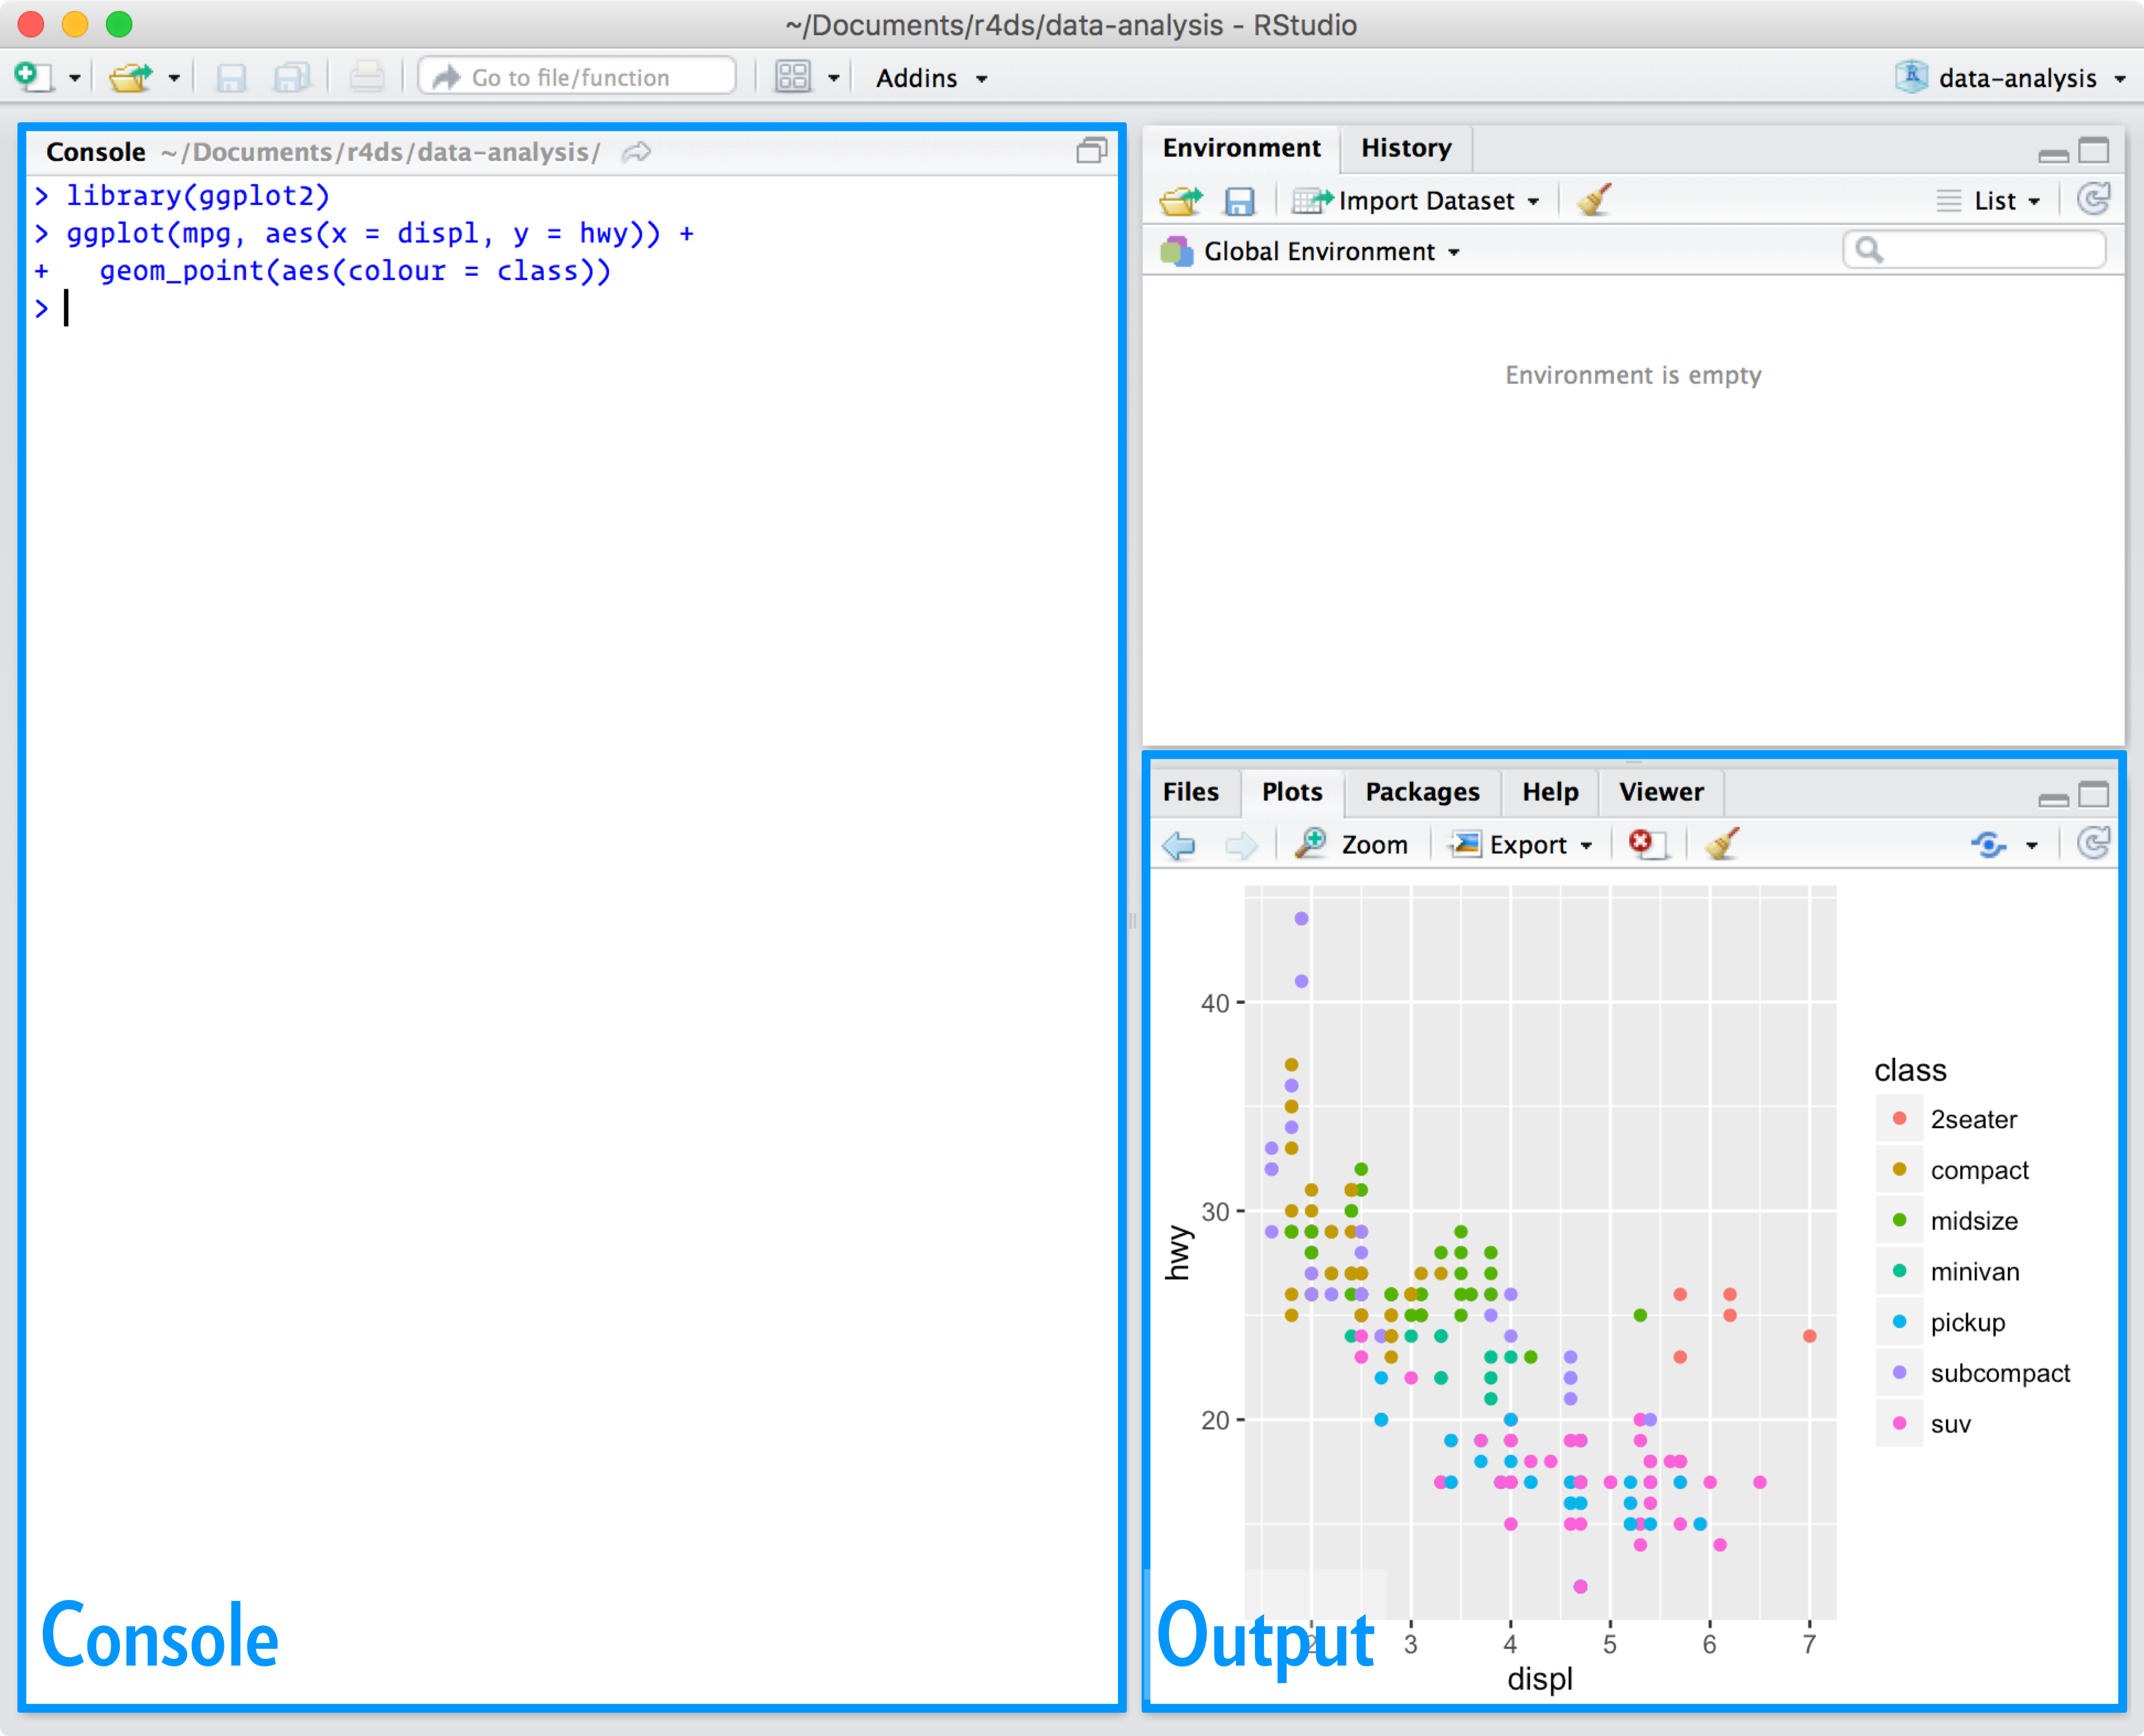
\includegraphics[width=1\linewidth]{images/rstudio-console} \end{center}

You can type R code into the \emph{Console} and press the enter key to run code.

\hypertarget{r-packages}{%
\section{R packages}\label{r-packages}}

An R package is a collection of R code and documentation that can be installed to enhance the standard R environment with additional functionality. Currently, there are over fifteen thousand R packages available on CRAN. Each of these R packages are developed to perform a specific task, such as \href{https://cran.r-project.org/web/packages/readxl/index.html}{reading Excel spreadsheets}, \href{https://cran.r-project.org/web/packages/MODIStsp/index.html}{downloading satellite imagery data}, \href{https://cran.r-project.org/web/packages/wdpar/index.html}{downloading and cleaning protected area data}, or \href{https://cran.r-project.org/web/packages/ENMeval/index.html}{fitting environmental niche models}. In fact, R has such a diverse ecosystem of R packages, that the question is almost always not ``can I use R to \ldots?'' but ``what R package can I use to \ldots?''. During this workshop, we will use several R packages. To install these R packages, please enter the code below in the \emph{Console} part of the RStudio interface and press enter. Note that you will require an Internet connection and the installation process may take some time to complete.

\begin{Shaded}
\begin{Highlighting}[]
\FunctionTok{install.packages}\NormalTok{(}\FunctionTok{c}\NormalTok{(}\StringTok{"sf"}\NormalTok{, }\StringTok{"dplyr"}\NormalTok{, }\StringTok{"sp"}\NormalTok{, }\StringTok{"rgeos"}\NormalTok{, }\StringTok{"rgdal"}\NormalTok{, }\StringTok{"raster"}\NormalTok{,}
                   \StringTok{"units"}\NormalTok{, }\StringTok{"prioritizr"}\NormalTok{, }\StringTok{"prioritizrdata"}\NormalTok{,}
                   \StringTok{"mapview"}\NormalTok{, }\StringTok{"assertthat"}\NormalTok{, }\StringTok{"remotes"}\NormalTok{, }\StringTok{"gridExtra"}\NormalTok{,}
                   \StringTok{"BiocManager"}\NormalTok{))}
\NormalTok{BiocManager}\SpecialCharTok{::}\FunctionTok{install}\NormalTok{(}\StringTok{"lpsymphony"}\NormalTok{)}
\end{Highlighting}
\end{Shaded}

Some of the new code in this workshop relies on \emph{prioritizr R} package v6.0 which is only available on Github at the moment. The CRAN version is currently 5.03. You do not have to install v6.0 if you don't wish to. There are only a few instances of code which will not be able to run. But if you want to try v6.0 you can run:

\begin{Shaded}
\begin{Highlighting}[]
\NormalTok{devtools}\SpecialCharTok{::}\FunctionTok{install\_github}\NormalTok{(}\StringTok{"prioritizr/prioritizr"}\NormalTok{)}
\end{Highlighting}
\end{Shaded}

This will require you to have all the tools required for building packages installed on your computer but RStudio should help with the process and you can get help from here: \url{https://support.rstudio.com/hc/en-us/articles/200486498-Package-Development-Prerequisites}.

\hypertarget{optimisation-software}{%
\section{Optimisation Software}\label{optimisation-software}}

While it possible to use the \texttt{lpsymphony} package installed above, \emph{Gurobi} is the most powerful and fastest solver that the \emph{prioritizr R} package can use to solve conservation planning problems. This section will walk you through the process of setting up \emph{Gurobi} on your computer. If you encounter any problems while following the instructions below, check out the \href{https://www.gurobi.com/documentation/}{official \emph{Gurobi} documentation}. If you can't solve the problems, don't worry. We can use \texttt{lpsymphony}.

\hypertarget{obtaining-a-license}{%
\subsection{Obtaining a license}\label{obtaining-a-license}}

\emph{Gurobi} is a commercial computer program. \href{https://www.gurobi.com/products/licensing-pricing/licensing-overview}{This means that users will need to obtain a license for \emph{Gurobi} before they can use it}. Although academics can obtain a special license at no cost, individuals that are not affiliated with a recognized educational institution may need to purchase a license to use \emph{Gurobi}. If you are an academic that is affiliated with an educational institution, you can take advantage of the \href{https://www.gurobi.com/downloads/end-user-license-agreement-academic/}{special academic license} to use \emph{Gurobi} for no cost. Once you have signed up for a free account you can request a \href{https://www.gurobi.com/downloads/end-user-license-agreement-academic/}{free academic license}.


\includegraphics[width=0.75\textwidth,height=\textheight]{images/free-academic-license-page.png}

Once you accept the Terms Of Service you can generate a license.

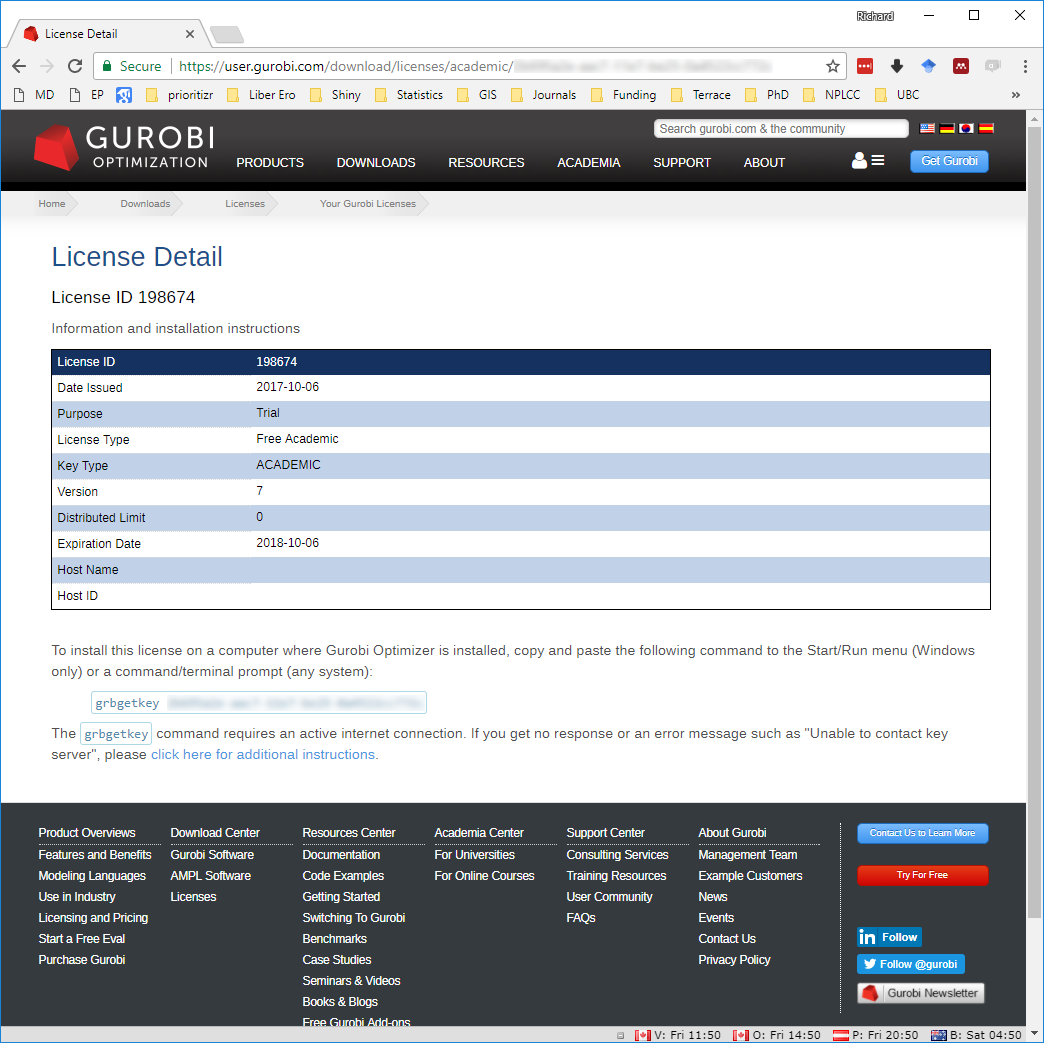
\includegraphics[width=0.75\textwidth,height=\textheight]{images/actual-license.png}

Now, copy and save the \texttt{grbgetkey\ XXXXXXXX-XXXX-XXXX-XXXX-XXXXXXXXXXXX} command for later use.

\hypertarget{downloading-the-gurobi-software-suite}{%
\subsection{\texorpdfstring{Downloading the \emph{Gurobi} software suite}{Downloading the Gurobi software suite}}\label{downloading-the-gurobi-software-suite}}

After obtaining a license, you will need to download a copy of the \emph{Gurobi} installer to your computer. To achieve this, visit the \href{https://www.gurobi.com/downloads/gurobi-optimizer}{\emph{Gurobi} downloads web page} and download the correct version of the installer for your operating system.

\hypertarget{software-installation}{%
\subsection{Software installation}\label{software-installation}}

The installation process for the \emph{Gurobi} software suite depends on the type of operating system you have installed on your computer. Fortunately, \emph{Gurobi} provide platform-specific \href{https://www.gurobi.com/documentation/}{``Quick Start Guides''} for \href{https://www.gurobi.com/documentation/8.1/quickstart_windows/software_installation_guid.html\#section:Installation}{Windows}, \href{https://www.gurobi.com/documentation/8.1/quickstart_mac/software_installation_guid.html}{Mac OSX}, and \href{https://www.gurobi.com/documentation/8.1/quickstart_linux/software_installation_guid.html}{Linux} systems that should help with this. Briefly, on Windows and Mac systems, you just need to double-click on the \emph{Gurobi} installer, follow the prompts, and the installer will take care of rest.

After installing the \emph{Gurobi} software suite on your computer, you will need to activate your license.

\hypertarget{license-activation}{%
\subsection{License activation}\label{license-activation}}

Now we will activate the \emph{Gurobi} software using the license you downloaded earlier. Please note that the correct set of instructions depends on your system and license. In most cases, you should follow the instructions in the ``Local license activation''. If, and only if, you are activating a special Academic license on a networked computer that is not connected to your university's network (e.g.~a cloud-based system), then please follow the instructions below in the ``Cloud license activation over SSH'' section.

\hypertarget{local-license-activation}{%
\subsection{Local license activation}\label{local-license-activation}}

To activate the license, simply copy and paste the \texttt{grbgetkey} command into your computer's command prompt or terminal (note that Windows users can open the command prompt by typing \texttt{cmd} in the search box and pressing the \texttt{enter} key). After running the \texttt{grbgetkey} command with the correct license code, you should see output that looks something like that in the screen shot below.

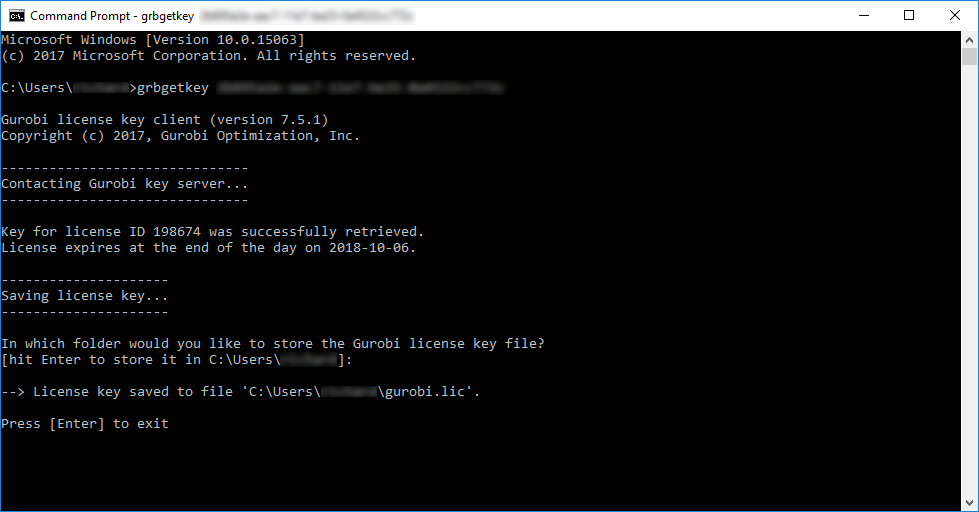
\includegraphics[width=0.75\textwidth,height=\textheight]{images/cmd-windows-success.png}

\hypertarget{install-gurobi-r}{%
\subsection{Install gurobi R}\label{install-gurobi-r}}

To install the R package, instructions can be found \href{https://www.gurobi.com/documentation/9.1/refman/ins_the_r_package.html}{here}. Briefly you can install it by substituting \texttt{\textless{}R-package-file\textgreater{}} in the code below for the location of the Gurobi software on your computer.

\begin{Shaded}
\begin{Highlighting}[]
\FunctionTok{install.packages}\NormalTok{(}\StringTok{\textquotesingle{}\textless{}R{-}package{-}file\textgreater{}\textquotesingle{}}\NormalTok{, }\AttributeTok{repos=}\ConstantTok{NULL}\NormalTok{)}

\CommentTok{\# For a Mac it would be:}
\FunctionTok{install.packages}\NormalTok{(}\StringTok{"/Library/gurobi911/mac64/R/gurobi\_9.1{-}1\_R\_4.0.2.tgz"}\NormalTok{, }\AttributeTok{repos =} \ConstantTok{NULL}\NormalTok{)}
\end{Highlighting}
\end{Shaded}

Depending on your local R environment you might need to install the R package slam. To do this, you should issue the following command within R:

\begin{Shaded}
\begin{Highlighting}[]
\FunctionTok{install.packages}\NormalTok{(}\StringTok{\textquotesingle{}slam\textquotesingle{}}\NormalTok{)}
\end{Highlighting}
\end{Shaded}

\hypertarget{test-your-install}{%
\section{Test your install}\label{test-your-install}}

You can check if you have successfully installed Gurobi by running the code below. If you don't get any errors, you are good to go. Don't worry about what it means. That is what we are going to learn.

\begin{Shaded}
\begin{Highlighting}[]
\FunctionTok{library}\NormalTok{(prioritizr)}

\FunctionTok{data}\NormalTok{(sim\_pu\_raster)}
\FunctionTok{data}\NormalTok{(sim\_features)}

\NormalTok{p }\OtherTok{\textless{}{-}} \FunctionTok{problem}\NormalTok{(sim\_pu\_raster, sim\_features) }\SpecialCharTok{\%\textgreater{}\%}
  \FunctionTok{add\_min\_set\_objective}\NormalTok{() }\SpecialCharTok{\%\textgreater{}\%}
  \FunctionTok{add\_binary\_decisions}\NormalTok{() }\SpecialCharTok{\%\textgreater{}\%}
  \FunctionTok{add\_relative\_targets}\NormalTok{(}\FloatTok{0.1}\NormalTok{) }\SpecialCharTok{\%\textgreater{}\%}
  \FunctionTok{add\_gurobi\_solver}\NormalTok{(}\AttributeTok{verbose =} \ConstantTok{FALSE}\NormalTok{)}

\NormalTok{s }\OtherTok{\textless{}{-}} \FunctionTok{solve}\NormalTok{(p)}
\end{Highlighting}
\end{Shaded}

If you couldn't install Gurobi, and instead went with lpsymphony, try substituting \texttt{add\_gurobi\_solver(verbose\ =\ FALSE)} with \texttt{add\_lpsymphony\_solver(verbose\ =\ FALSE)}.

\hypertarget{overview-of-the-conservation-planning-problem}{%
\chapter{Overview of the conservation planning problem}\label{overview-of-the-conservation-planning-problem}}

\hypertarget{summary}{%
\section{Summary}\label{summary}}

The \emph{prioritizr R} package uses integer linear programming (ILP) techniques to provide a flexible interface for building and solving conservation planning problems \citep{r11, r16}. It supports a broad range of objectives, constraints, and penalties that can be used to customize conservation planning problems to the specific needs of a conservation planning exercise.

Once built, conservation planning problems can be solved using a variety of commercial and open-source exact algorithm solvers. In contrast to the algorithms conventionally used to solve conservation problems, such as heuristics or simulated annealing \citep{r3}, the exact algorithms used here are guaranteed to find optimal solutions.

Furthermore, conservation problems can be constructed to optimize the spatial allocation of different management zone (or actions), meaning that conservation practitioners can identify solutions that benefit multiple stakeholders.

\hypertarget{introduction}{%
\section{Introduction}\label{introduction}}

Systematic conservation planning is a rigorous, repeatable, and structured approach to designing new protected areas that efficiently meet conservation objectives \citep{r4}.

Historically, conservation decision-making has often evaluated parcels opportunistically as they became available for purchase, donation, or under threat. Although purchasing such areas may improve the \emph{status quo}, such decisions may not substantially enhance the long-term persistence of target species or communities.

Therefore conservation planners began using decision support tools to help simulate alternative reserve designs over a range of different biodiversity and management goals and, ultimately, guide protected area acquisitions and management actions. Due to the systematic, evidence-based nature of these tools, \textbf{conservation prioritization can help contribute to a transparent, inclusive, and more defensible decision making process}.

\hypertarget{overall-concepts}{%
\subsection{Overall Concepts}\label{overall-concepts}}

There are several concepts that underpin the conservation planning problems. Some of them are:

\begin{itemize}
\tightlist
\item
  \textbf{Study Area}: A conservation planning exercise typically starts by defining a study area. This study area should encompass all the areas relevant to the decision maker or the hypothesis being tested. The extent of a study area could encompass a few important localities \citep[e.g.][]{r18}, a single state \citep[e.g.][]{r17}, an entire country \citep{r19}, or the entire planet \citep{r20}.
\item
  \textbf{Planning units}: Planning units are the building blocks of a reserve system. Each planning unit represents a discrete locality in the study area that can be managed independently of other areas. The general idea is that some combination of the planning units can be selected for conservation actions (e.g.~protected area establishment, habitat restoration). Planning units are often created as square or hexagon cells that are sized according to the scale of the conservation actions, and the resolution of the data that underpin the planning exercise \citep[but see][]{r5}.
\item
  \textbf{Features}: A conservation feature is a measurable, spatially definable component of biodiversity that is to be conserved within a reserve network (e.g., species, communities, habitat types, populations, etc.). After identifying the set of relevant conservation features for a conservation planning exercise, spatially explicit data need to be obtained for each and every feature to describe their spatial distribution (e.g.~habitat suitability data, probability of occurrence data, presence/absence data). This is important to ensure that conservation features are adequately covered (represented) by prioritizations.
\item
  \textbf{Target}: Each conservation feature is given a target. Targets are the quantitative values (amounts) of each conservation feature to be achieved in the final reserve solution
\item
  \textbf{Cost}: The cost of including a planning unit in a reserve system. This cost should reflect the socio-political constraints to setting aside that planning unit for conservation actions. This could be: total area, cost of acquisition or any other relative social, economic or ecological measure (e.g loss of fishing or logging land). Each planning unit is assigned one cost (\emph{although several measures can be combined to create a cost metric})
\item
  \textbf{Objectives}: An objective is used to specify the overall goal of a conservation planning problem. All conservation planning problems involve minimizing or maximizing some kind of objective
\item
  \textbf{Penalties}: A penalty can be applied to a conservation planning problem to penalize solutions according to a specific metric. Penalties---unlike constraints---act as an explicit trade-off with the objective being minimized or maximized.
\item
  \textbf{Constraints}: Constraints can be used to ensure that solutions exhibit a range of different characteristics. For instance, they can be used to lock in or lock out certain planning units from the solution, such as protected areas or degraded land (respectively).
\item
  \textbf{Portfolios}: Conservation planning exercises rarely have access to all the data needed to identify the truly perfect solution. This is because available data may lack important details or contain errors. As such, conservation planners can help decision makers by providing them with a portfolio of solutions to inform their decision.
\end{itemize}

\hypertarget{choosing-marine-reserves-the-c.a.r.e.-approach}{%
\subsection{Choosing Marine Reserves: The C.A.R.E. Approach}\label{choosing-marine-reserves-the-c.a.r.e.-approach}}

\hypertarget{the-optimisation-problem}{%
\subsection{The Optimisation Problem}\label{the-optimisation-problem}}

The \emph{prioritizr R} package is designed to help you build and solve conservation planning problems. Specifically, prioritizations are generated by using formulating a mathematical optimization problem and then solving it to generate a solution. These mathematical optimization problems are formulated using the planning unit data, cost data, and feature data, and with information related to the overarching aim of the prioritization process.

In general, the goal of an optimization problem is to minimize (or maximize) an \emph{objective function} that is calculated using a set of \emph{decision variables}, subject to a series of \emph{constraints} to ensure that solution exhibits specific properties. The \emph{objective function} describes the quantity which we are trying to minimize (e.g.~cost of the solution) or maximize (e.g.~number of features conserved). The \emph{decision variables} describe the entities that we can control, and indicate which planning units are selected for conservation management and which of those are not. The \emph{constraints} can be thought of as rules that the need decision variables need to follow.

\begin{figure}

{\centering 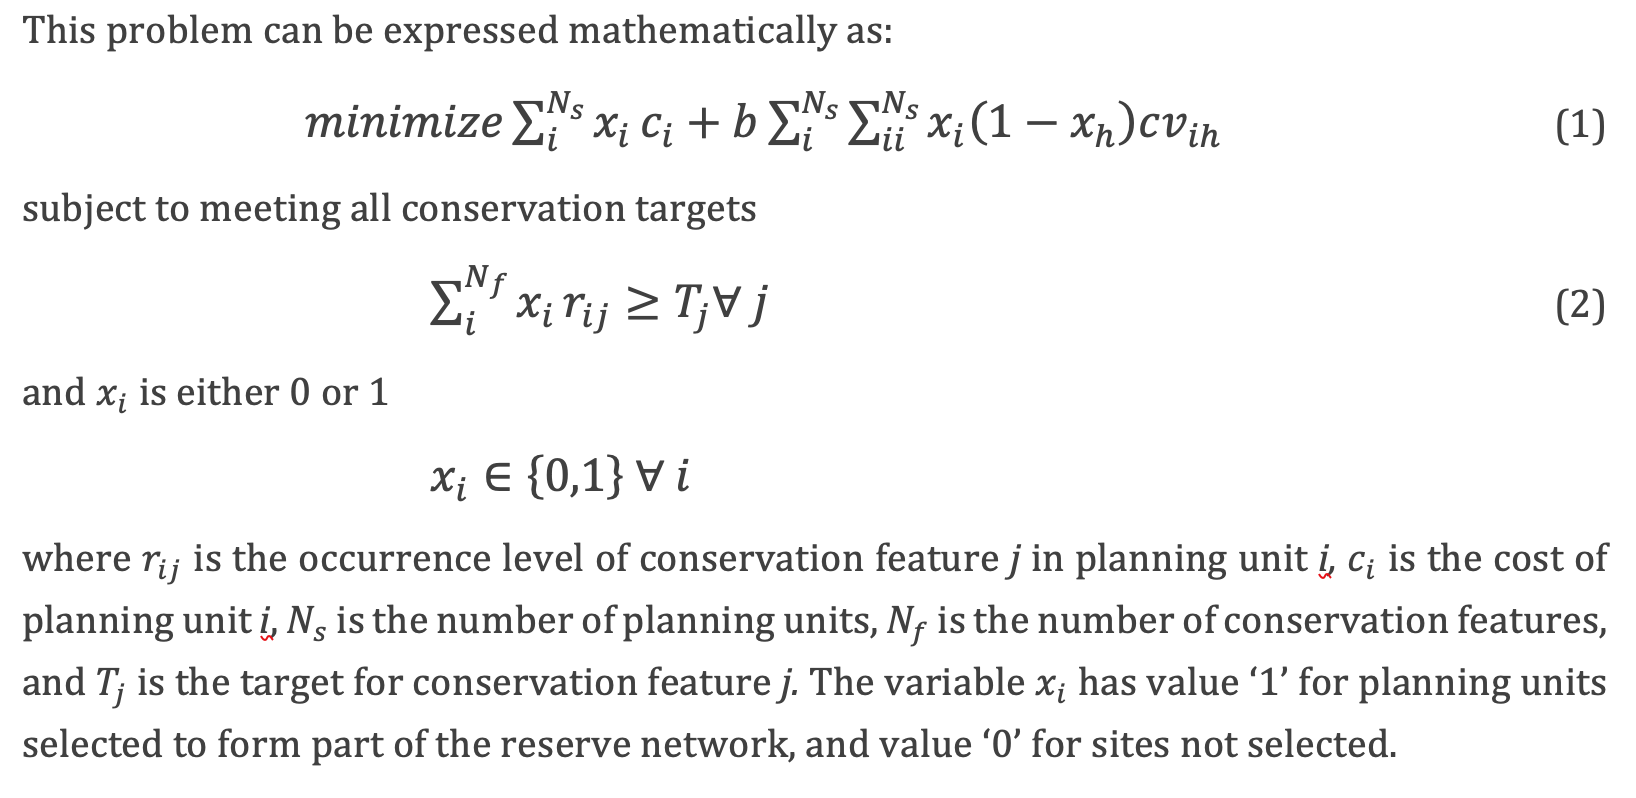
\includegraphics[width=1\linewidth]{images/Equation} 

}

\caption{Prioritizr problem equation}(\#fig:Problem equation)
\end{figure}

\begin{figure}

{\centering 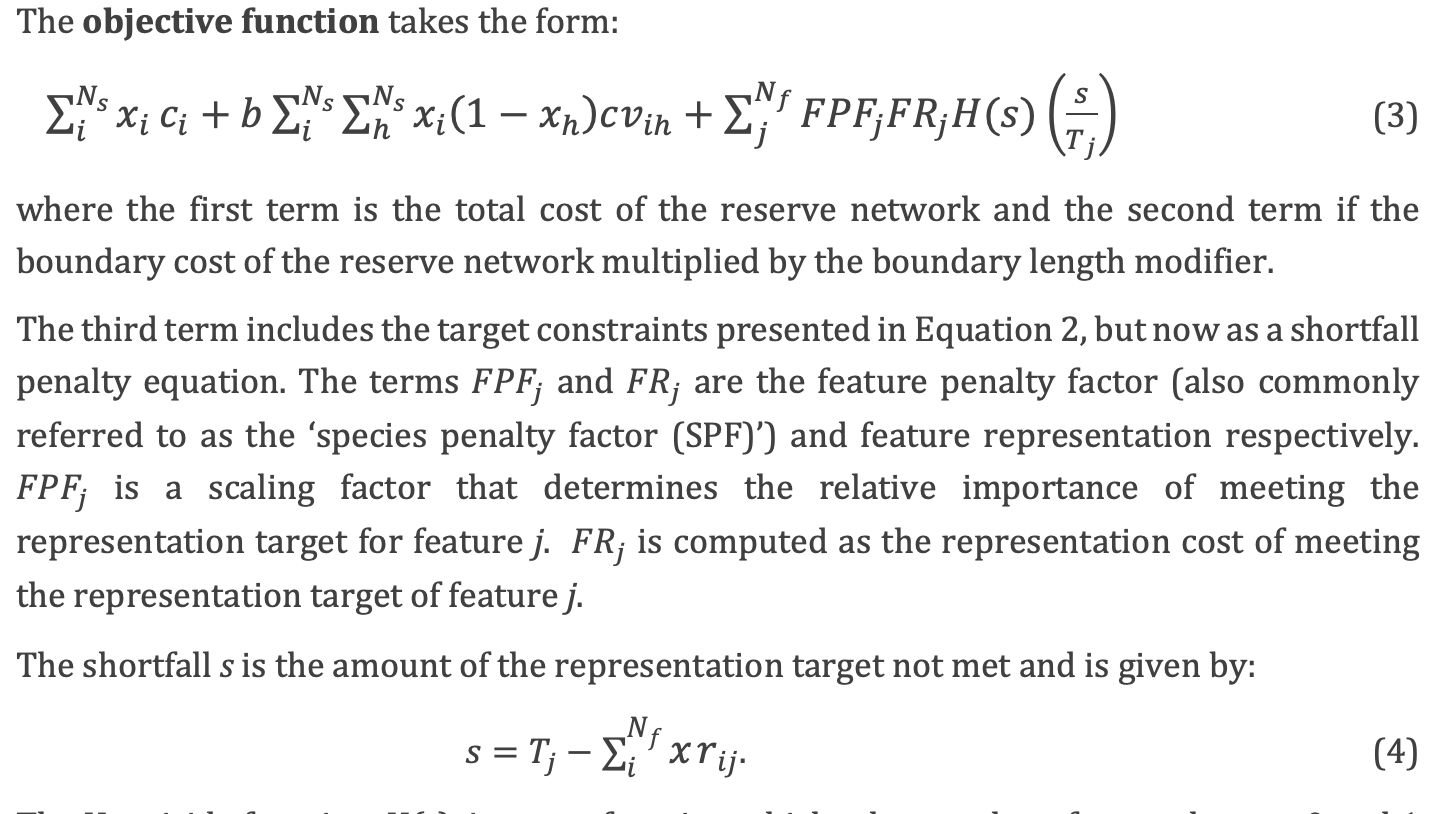
\includegraphics[width=1\linewidth]{images/Objective} 

}

\caption{Prioritizr Objective}\label{fig:Objective}
\end{figure}

\begin{figure}

{\centering 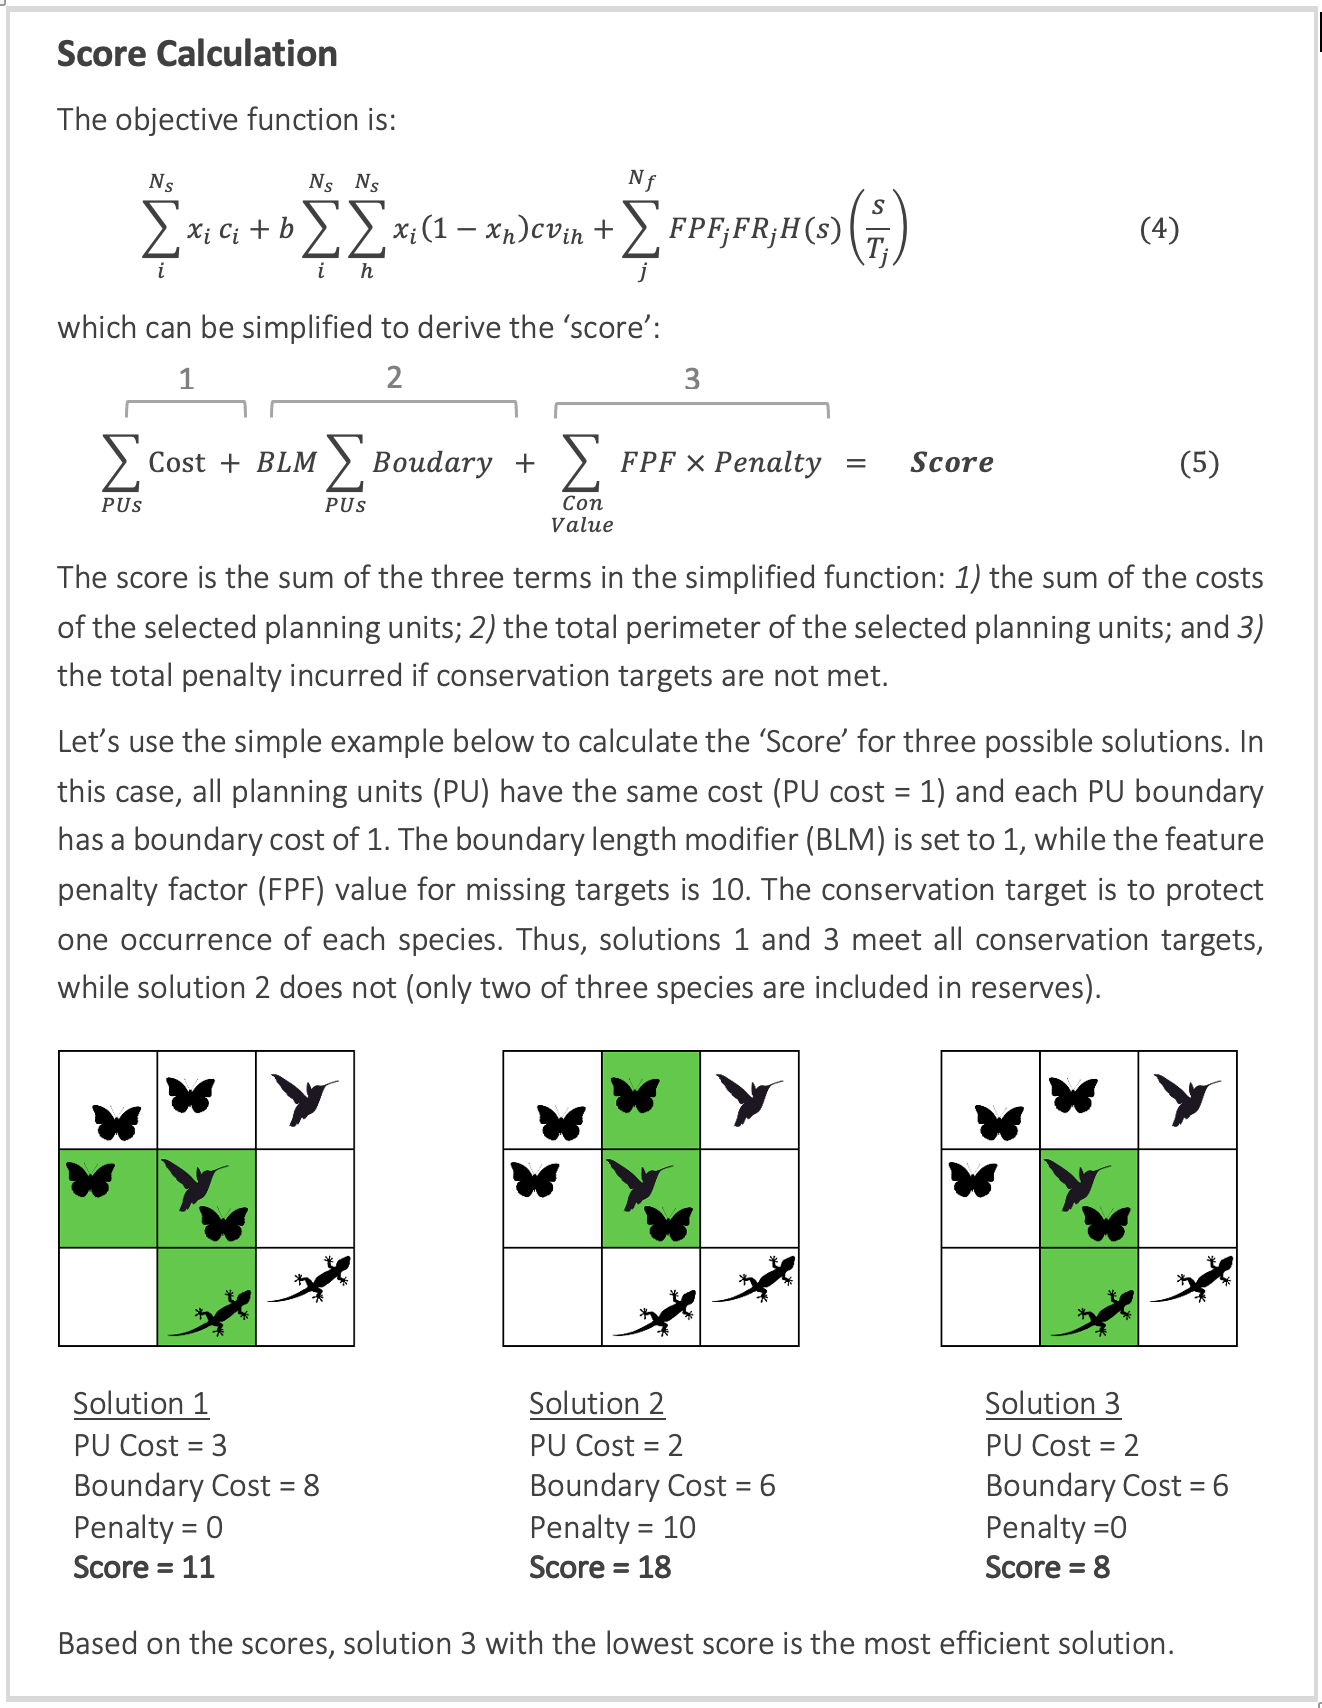
\includegraphics[width=1\linewidth]{images/Box} 

}

\caption{Score Calculation}\label{fig:Box}
\end{figure}

A wide variety of approaches have been developed for solving optimization problems. Reserve design problems are frequently solved using simulated annealing \citep{r6} or heuristics \citep{r8, r7}. These methods are conceptually simple and can be applied to a wide variety of optimization problems. However, they do not scale well for large or complex problems \citep{r1}. Additionally, these methods cannot tell you how close any given solution is to the optimal solution.

The \emph{prioritizr R} package uses exact algorithms to efficiently solve conservation planning problems to within a pre-specified a optimality gap. In other words, you can specify that you need the optimal solution (i.e.~a gap of 0\%) and the algorithms will, given enough time, find a solution that meets this criteria.

In the past, exact algorithms have been too slow for conservation planning exercises \citep{r9}. However, improvements over the last decade mean that they are now much faster \citep{r23, r1}. In this package, optimization problems are expressed using \emph{integer linear programming} (ILP) so that they can be solved using (linear) exact algorithm solvers.

\hypertarget{getting-started-with-prioritizr}{%
\chapter{Getting Started with Prioritizr}\label{getting-started-with-prioritizr}}

\hypertarget{package-overview}{%
\section{Package overview}\label{package-overview}}

The \emph{prioritizr R} package contains eight main types of functions. These functions are used to:

\begin{itemize}
\tightlist
\item
  create a new conservation planning \href{https://prioritizr.net/reference/problem.html}{problem} by specifying the planning units, features, and management zones of conservation interest (e.g.~species, ecosystems).
\item
  add an \href{https://prioritizr.net/reference/objectives.html}{objective} to a conservation planning problem.
\item
  add \href{https://prioritizr.net/reference/targets.html}{targets} to a problem to specify how much of each feature is desired or required to be conserved in the solutions.
\item
  add \href{https://prioritizr.net/reference/constraints.html}{constraints} to a conservation planning problem to ensure that solutions exhibit specific properties (e.g.~select specific planning units for protection).
\item
  add \href{https://prioritizr.net/reference/penalties.html}{penalties} to a problem to penalize solutions according to specific metric (e.g.~connectivity).
\item
  add \href{https://prioritizr.net/reference/decisions.html}{decisions} to a problem to specify the nature of the decisions in the problem.
\item
  add methods to generate a \href{https://prioritizr.net/reference/portfolios.html}{portfolio} of solutions.
\item
  add a \href{https://prioritizr.net/reference/solvers.html}{solver} to a conservation problem to specify which software should be used to generate solutions and customize the optimization process.
\item
  \href{https://prioritizr.net/reference/solve.html}{solve} a conservation problem.
\item
  evaluate a solution by computing \href{https://prioritizr.net/reference/summaries.html}{summary} statistics.
\item
  evaluate the relative \href{https://prioritizr.net/reference/importance.html}{importance} (irreplaceability) of planning units selected in a solution.
\end{itemize}

\hypertarget{package-work-flow}{%
\section{Package work flow}\label{package-work-flow}}

The general work flow when using the \emph{prioritizr R} package starts with creating a new conservation planning \texttt{problem} object using data. Specifically, the \texttt{problem} object should be constructed using data that specify:\\
* the planning units,\\
* biodiversity features,\\
* management zones (if applicable), and\\
* costs.

After creating a new \texttt{problem} object, it can be customized by adding:\\
* objectives,\\
* penalties and constraints
to build a precise representation of the conservation planning problem required.

It is then solved to obtain a solutions.

\hypertarget{objectives}{%
\subsection{Objectives}\label{objectives}}

All conservation planning problems require an objective. An objective specifies the property which is used to compare different feasible solutions. Simply put, the objective is the property of the solution which should be maximized or minimized during the optimization process. For instance:\\
* with the minimum set objective (specified using \texttt{add\_min\_set\_objective}), we are seeking to minimize the cost of the solution (similar to \emph{Marxan})\\
* with the maximum coverage objective (specified using \texttt{add\_max\_cover\_objective}), we are seeking to maximize the number of different features represented in the solution.

Many objectives require \texttt{targets} (e.g.~the minimum set objective). Targets are a specialized set of constraints that relate to the total quantity of each feature secured in the solution (e.g.~amount of suitable habitat or number of individuals). Fo example:\\
* the minimum set objective ( \texttt{add\_min\_set\_objective}) are used to ensure that solutions secure a sufficient quantity of each feature\\
* the maximum features objective ( \texttt{add\_max\_features\_objective}) are used to assess whether a feature has been adequately conserved by a candidate solution.

Targets can be expressed:\\
* numerically as the total amount required for a given feature (using \texttt{add\_absolute\_targets}), or as\\
* a proportion of the total amount found in the planning units (using \texttt{add\_relative\_targets}).

\textbf{Note} not all objectives require targets, and a warning will be thrown if an attempt is made to add targets to a problem with an objective that does not use them.

\hypertarget{penaltes-and-constraints}{%
\subsection{Penaltes and Constraints}\label{penaltes-and-constraints}}

Constraints and penalties can be added to a conservation planning problem to ensure that solutions exhibit a specific property or penalize solutions which don't exhibit a specific property (respectively).\\
* \textbf{Constraints} are used to rule out potential solutions that don't exhibit a specific property. For instance, constraints can be used to ensure that specific planning units are selected in the solution for prioritization (using \texttt{add\_locked\_in\_constraints}) or not selected in the solution for prioritization (using \texttt{add\_locked\_out\_constraints}).\\
* \textbf{Penalties} are combined with the objective of a problem, with a penalty factor, and the overall objective of the problem then becomes to minimize (or maximize) the primary objective function and the penalty function. For example, penalties can be added to a problem to penalize solutions that are excessively fragmented (using \texttt{add\_boundary\_penalties}). These penalties have a \texttt{penalty} argument that specifies the relative importance of having spatially clustered solutions. When the argument to \texttt{penalty} is high, then solutions which are less fragmented are valued more highly---even if they cost more---and when the argument to \texttt{penalty} is low, then the solutions which are more fragmented are valued less highly.

After building a conservation problem, it can then be solved to obtain a solution (or portfolio of solutions if desired). The solution is returned in the same format as the planning unit data used to construct the problem. This means that if raster or shapefile / vector data was used when initializing the problem, then the solution will also be in raster or shapefile / vector data.

\hypertarget{usage}{%
\section{Usage}\label{usage}}

Here we will provide an introduction to using the \emph{prioritizr R} package to build and solve a conservation planning problem.

First, we will load the \emph{prioritizr} package.

\begin{Shaded}
\begin{Highlighting}[]
\CommentTok{\# load package}
\FunctionTok{library}\NormalTok{(prioritizr)}

\CommentTok{\# set default options for printing tabular data}
\FunctionTok{options}\NormalTok{(}\AttributeTok{tibble.width =} \ConstantTok{Inf}\NormalTok{)}
\end{Highlighting}
\end{Shaded}

\hypertarget{simulated-data}{%
\subsection{Simulated Data}\label{simulated-data}}

Now we will load some built-in data sets that are distributed with the \emph{prioritizr R} package. This package contains several different planning unit data sets. To provide a comprehensive overview of the different ways that we can initialize a conservation planning problem, we will load each of them.

First, we will load the raster planning unit data (\texttt{sim\_pu\_raster}). Here, the planning units are represented as a raster (i.e.~a \texttt{RasterLayer} object) and each pixel corresponds to the spatial extent of each planning unit. The pixel values correspond to the acquisition costs of each planning unit.

\begin{Shaded}
\begin{Highlighting}[]
\CommentTok{\# load raster planning unit data}
\FunctionTok{data}\NormalTok{(sim\_pu\_raster)}

\CommentTok{\# print description of the data}
\FunctionTok{print}\NormalTok{(sim\_pu\_raster)}
\end{Highlighting}
\end{Shaded}

\begin{verbatim}
## class      : RasterLayer 
## dimensions : 10, 10, 100  (nrow, ncol, ncell)
## resolution : 0.1, 0.1  (x, y)
## extent     : 0, 1, 0, 1  (xmin, xmax, ymin, ymax)
## crs        : NA 
## source     : memory
## names      : layer 
## values     : 190.1328, 215.8638  (min, max)
\end{verbatim}

\begin{Shaded}
\begin{Highlighting}[]
\CommentTok{\# plot the data}
\FunctionTok{plot}\NormalTok{(sim\_pu\_raster)}
\end{Highlighting}
\end{Shaded}

\begin{center}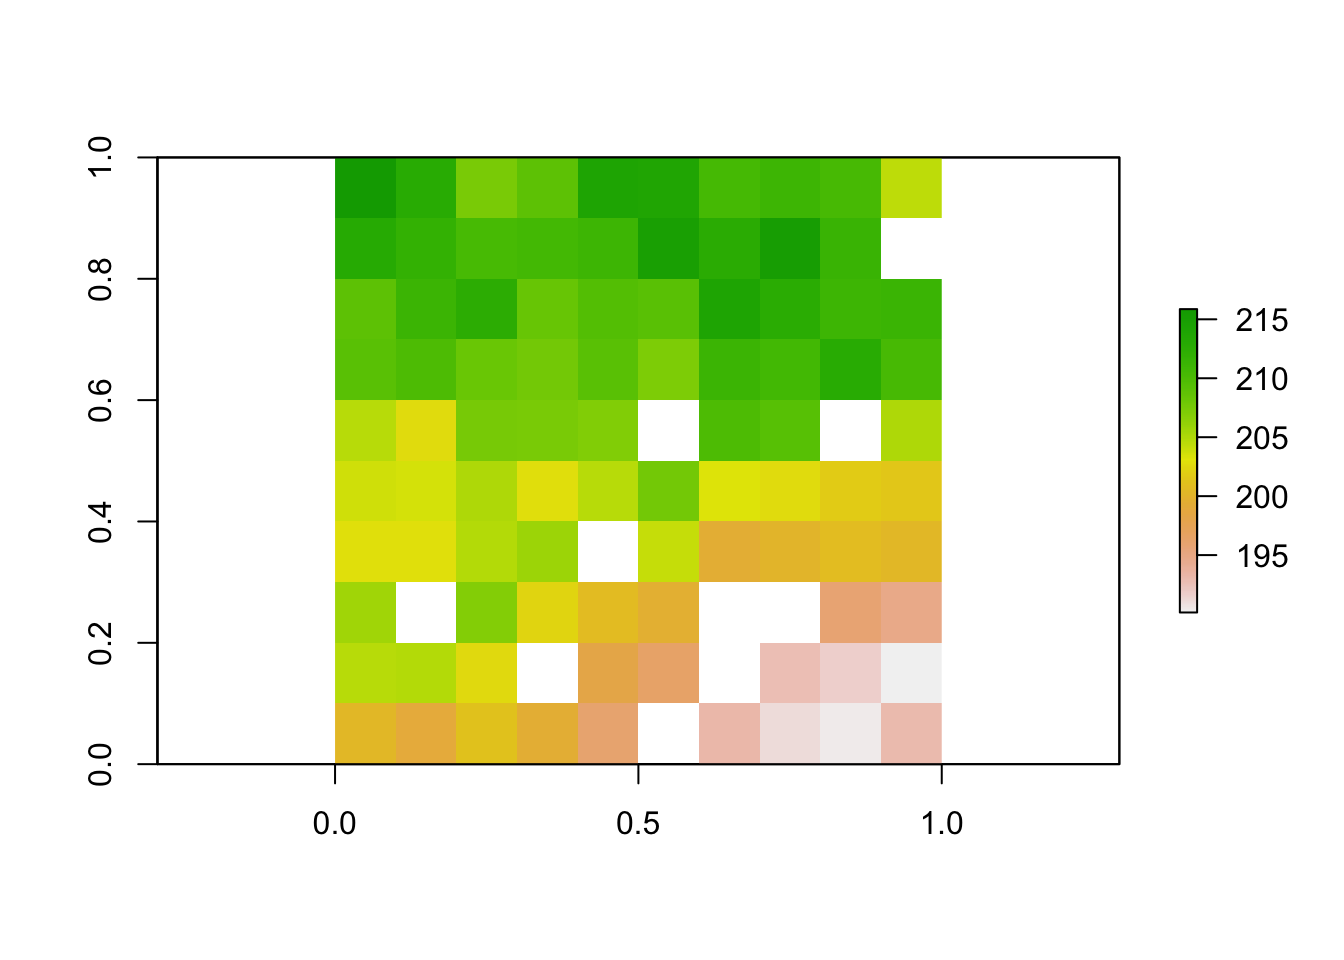
\includegraphics{SpatialPlanning_Workshop2021_files/figure-latex/unnamed-chunk-9-1} \end{center}

Secondly, we will load one of the spatial vector planning unit data sets (\texttt{sim\_pu\_polygons}). Here, each polygon (i.e.~feature using ArcGIS terminology) corresponds to a different planning unit. This data set has an attribute table that contains additional information about each polygon. Namely, the \texttt{cost} field (column) in the attribute table contains the acquisition cost for each planning unit.

\begin{Shaded}
\begin{Highlighting}[]
\CommentTok{\# load polygon planning unit data}
\FunctionTok{data}\NormalTok{(sim\_pu\_polygons)}

\CommentTok{\# print first six rows of attribute table}
\FunctionTok{head}\NormalTok{(sim\_pu\_polygons}\SpecialCharTok{@}\NormalTok{data)}
\end{Highlighting}
\end{Shaded}

\begin{verbatim}
##       cost locked_in locked_out
## 1 215.8638     FALSE      FALSE
## 2 212.7823     FALSE      FALSE
## 3 207.4962     FALSE      FALSE
## 4 208.9322     FALSE       TRUE
## 5 214.0419     FALSE      FALSE
## 6 213.7636     FALSE      FALSE
\end{verbatim}

\begin{Shaded}
\begin{Highlighting}[]
\CommentTok{\# plot the planning units}
\FunctionTok{spplot}\NormalTok{(sim\_pu\_polygons, }\AttributeTok{zcol =} \StringTok{"cost"}\NormalTok{)}
\end{Highlighting}
\end{Shaded}

\begin{center}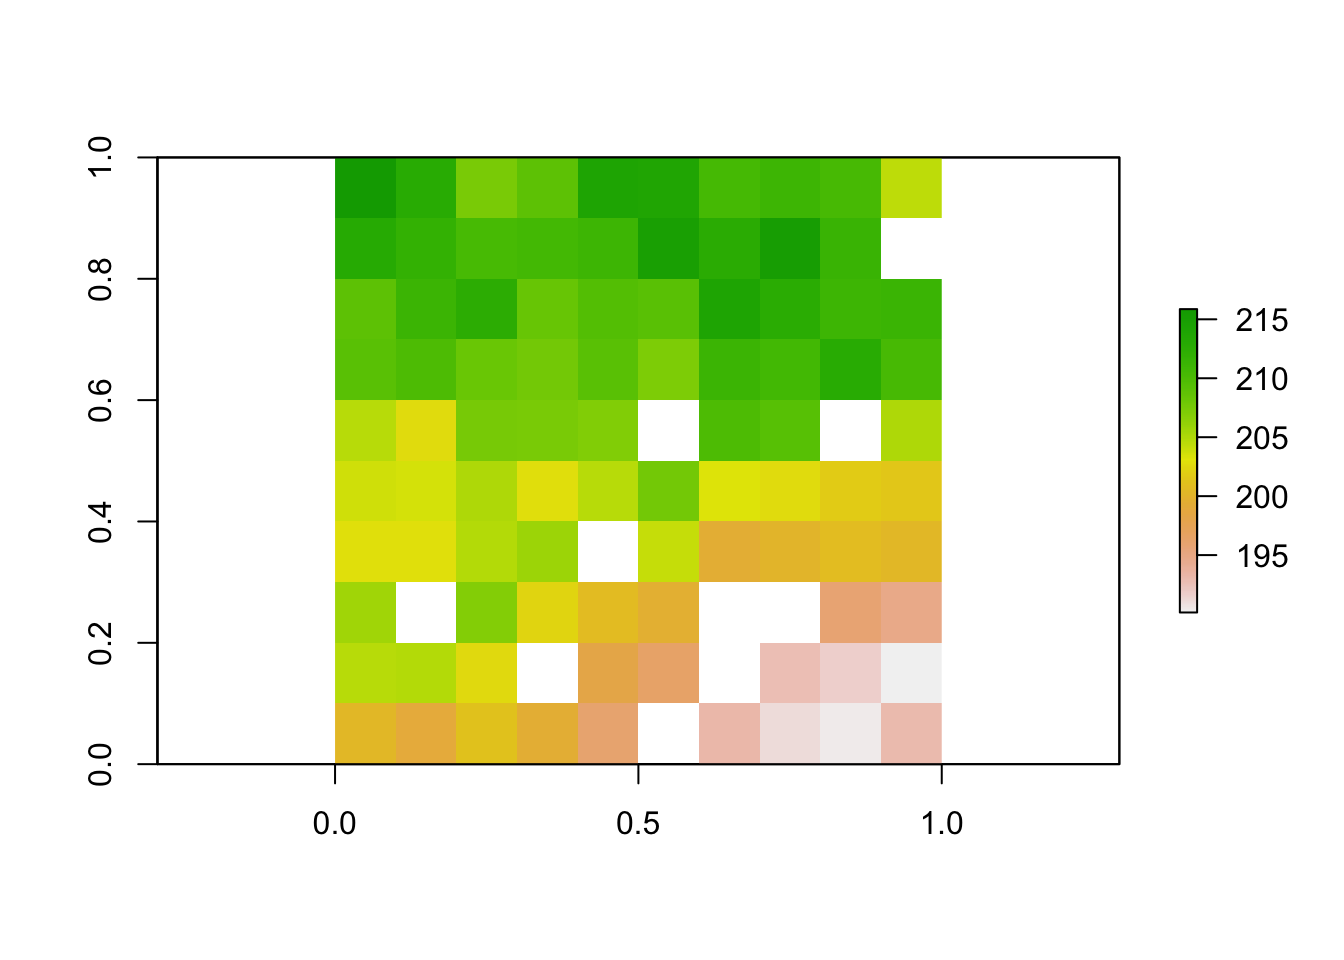
\includegraphics{SpatialPlanning_Workshop2021_files/figure-latex/unnamed-chunk-10-1} \end{center}

Thirdly, we will load some planning unit data stored in tabular format (i.e.~\texttt{data.frame} format). Each row in the planning unit table must correspond to a different planning unit. The table must also have an ``id'' column to provide a unique integer identifier for each planning unit, and it must also have a column that indicates the cost of each planning unit.

\begin{Shaded}
\begin{Highlighting}[]
\CommentTok{\# specify file path for planning unit data}
\NormalTok{pu\_path }\OtherTok{\textless{}{-}} \FunctionTok{system.file}\NormalTok{(}\StringTok{"extdata/input/pu.dat"}\NormalTok{, }\AttributeTok{package =} \StringTok{"prioritizr"}\NormalTok{)}

\CommentTok{\# load in the tabular planning unit data}
\CommentTok{\# note that we use the data.table::fread function, as opposed to the read.csv}
\CommentTok{\# function, because it is much faster}
\NormalTok{pu\_dat }\OtherTok{\textless{}{-}}\NormalTok{ data.table}\SpecialCharTok{::}\FunctionTok{fread}\NormalTok{(pu\_path, }\AttributeTok{data.table =} \ConstantTok{FALSE}\NormalTok{)}

\CommentTok{\# preview first six rows of the tabular planning unit data}
\CommentTok{\# note that it has some extra columns other than id and cost as per the}
\CommentTok{\# Marxan format}
\FunctionTok{head}\NormalTok{(pu\_dat)}
\end{Highlighting}
\end{Shaded}

\begin{verbatim}
##   id       cost status    xloc     yloc
## 1  3        0.0      0 1116623 -4493479
## 2 30   752727.5      3 1110623 -4496943
## 3 56  3734907.5      0 1092623 -4500408
## 4 58  1695902.1      0 1116623 -4500408
## 5 84  3422025.6      0 1098623 -4503872
## 6 85 17890758.4      0 1110623 -4503872
\end{verbatim}

Finally, we will load data showing the spatial distribution of the conservation features. Our conservation features (\texttt{sim\_features}) are represented as a stack of raster objects (i.e.~a \texttt{RasterStack} object) where each layer corresponds to a different feature (e.g.~a multi-band GeoTIFF where each band corresponds to a different feature). The pixel values in each layer correspond to the amount of suitable habitat available in a given planning unit. Note that our planning unit raster layer and our conservation feature stack have exactly the same spatial properties (i.e.~resolution, extent, coordinate reference system) so their pixels line up perfectly.

\begin{Shaded}
\begin{Highlighting}[]
\CommentTok{\# load feature data}
\FunctionTok{data}\NormalTok{(sim\_features)}

\CommentTok{\# plot the distribution of suitable habitat for each feature}
\FunctionTok{plot}\NormalTok{(sim\_features, }\AttributeTok{main =} \FunctionTok{paste}\NormalTok{(}\StringTok{"Feature"}\NormalTok{, }\FunctionTok{seq\_len}\NormalTok{(}\FunctionTok{nlayers}\NormalTok{(sim\_features))),}
     \AttributeTok{nr =} \DecValTok{2}\NormalTok{, }\AttributeTok{box =} \ConstantTok{FALSE}\NormalTok{, }\AttributeTok{axes =} \ConstantTok{FALSE}\NormalTok{)}
\end{Highlighting}
\end{Shaded}

\begin{center}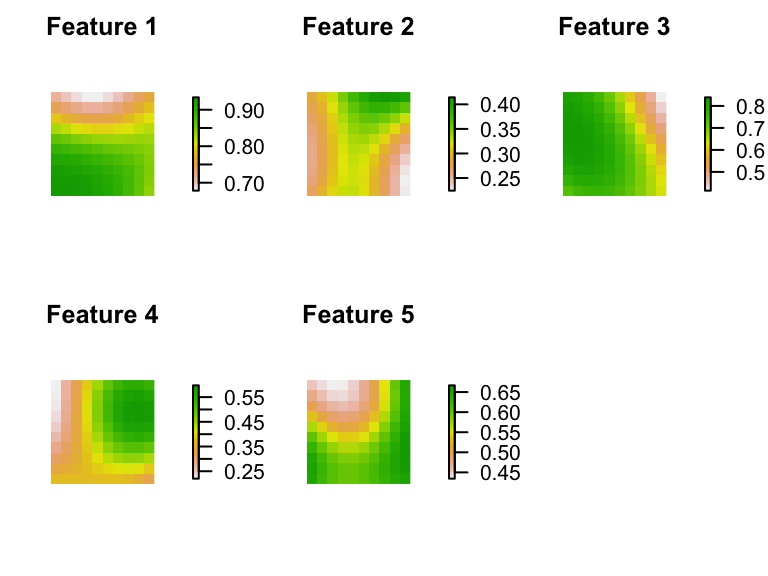
\includegraphics{SpatialPlanning_Workshop2021_files/figure-latex/unnamed-chunk-12-1} \end{center}

\hypertarget{initialize-a-problem}{%
\subsection{Initialize a problem}\label{initialize-a-problem}}

After having loaded our planning unit and feature data, we will now try initializing the some conservation planning problems. There are a lot of different ways to initialize a conservation planning problem, so here we will just showcase a few of the more commonly used methods. For an exhaustive description of all the ways you can initialize a conservation problem, see the help file for the \texttt{problem} function (which you can open using the code \texttt{?problem}).

First off, we will initialize a conservation planning problem using the raster data.

\begin{Shaded}
\begin{Highlighting}[]
\CommentTok{\# create problem}
\NormalTok{p1 }\OtherTok{\textless{}{-}} \FunctionTok{problem}\NormalTok{(sim\_pu\_raster, sim\_features)}

\CommentTok{\# print problem}
\FunctionTok{print}\NormalTok{(p1)}
\end{Highlighting}
\end{Shaded}

\begin{verbatim}
## Conservation Problem
##   planning units: RasterLayer (90 units)
##   cost:           min: 190.13276, max: 215.86384
##   features:       layer.1, layer.2, layer.3, ... (5 features)
##   objective:      none
##   targets:        none
##   decisions:      default
##   constraints:    <none>
##   penalties:      <none>
##   portfolio:      default
##   solver:         default
\end{verbatim}

\begin{Shaded}
\begin{Highlighting}[]
\CommentTok{\# print number of planning units}
\FunctionTok{number\_of\_planning\_units}\NormalTok{(p1)}
\end{Highlighting}
\end{Shaded}

\begin{verbatim}
## [1] 90
\end{verbatim}

\begin{Shaded}
\begin{Highlighting}[]
\CommentTok{\# print number of features}
\FunctionTok{number\_of\_features}\NormalTok{(p1)}
\end{Highlighting}
\end{Shaded}

\begin{verbatim}
## [1] 5
\end{verbatim}

Generally, we recommend initializing problems using raster data where possible. This is because the \texttt{problem} function needs to calculate the amount of each feature in each planning unit, and by providing both the planning unit and feature data in raster format with the same spatial resolution, extents, and coordinate systems, this means that the \texttt{problem} function does not need to do any geo-processing behind the scenes.

Sometimes we can't use raster planning unit data because our planning units aren't equal-sized grid cells. So, below is an example showing how we can initialize a conservation planning problem using planning units that are formatted as spatial vector data. Note that if we had pre-computed the amount of each feature in each planning unit and stored the data in the attribute table, we could pass in the names of the columns as an argument to the \texttt{problem} function.

\begin{Shaded}
\begin{Highlighting}[]
\CommentTok{\# create problem with spatial vector data}
\CommentTok{\# note that we have to specify which column in the attribute table contains}
\CommentTok{\# the cost data}
\NormalTok{p2 }\OtherTok{\textless{}{-}} \FunctionTok{problem}\NormalTok{(sim\_pu\_polygons, sim\_features, }\AttributeTok{cost\_column =} \StringTok{"cost"}\NormalTok{)}

\CommentTok{\# print problem}
\FunctionTok{print}\NormalTok{(p2)}
\end{Highlighting}
\end{Shaded}

\begin{verbatim}
## Conservation Problem
##   planning units: SpatialPolygonsDataFrame (90 units)
##   cost:           min: 190.13276, max: 215.86384
##   features:       layer.1, layer.2, layer.3, ... (5 features)
##   objective:      none
##   targets:        none
##   decisions:      default
##   constraints:    <none>
##   penalties:      <none>
##   portfolio:      default
##   solver:         default
\end{verbatim}

We can also initialize a conservation planning problem using tabular planning unit data (i.e.~a \texttt{data.frame}). Since the tabular planning unit data does not contain any spatial information, we also have to provide the feature data in tabular format (i.e.~a \texttt{data.frame}) and data showing the amount of each feature in each planning unit in tabular format (i.e.~a \texttt{data.frame}). The feature data must have an ``id'' column containing a unique integer identifier for each feature, and the planning unit by feature data must contain the following three columns: ``pu'' corresponding to the planning unit identifiers, ``species'' corresponding to the feature identifiers, and ``amount'' showing the amount of a given feature in a given planning unit.

\begin{Shaded}
\begin{Highlighting}[]
\CommentTok{\# set file path for feature data}
\NormalTok{spec\_path }\OtherTok{\textless{}{-}} \FunctionTok{system.file}\NormalTok{(}\StringTok{"extdata/input/spec.dat"}\NormalTok{, }\AttributeTok{package =} \StringTok{"prioritizr"}\NormalTok{)}

\CommentTok{\# load in feature data}
\NormalTok{spec\_dat }\OtherTok{\textless{}{-}}\NormalTok{ data.table}\SpecialCharTok{::}\FunctionTok{fread}\NormalTok{(spec\_path, }\AttributeTok{data.table =} \ConstantTok{FALSE}\NormalTok{)}

\CommentTok{\# print first six rows of the data}
\CommentTok{\# note that it contains extra columns}
\FunctionTok{head}\NormalTok{(spec\_dat)}
\end{Highlighting}
\end{Shaded}

\begin{verbatim}
##   id prop spf   name
## 1 10  0.3   1  bird1
## 2 11  0.3   1  nvis2
## 3 12  0.3   1  nvis8
## 4 13  0.3   1  nvis9
## 5 14  0.3   1 nvis14
## 6 15  0.3   1 nvis20
\end{verbatim}

\begin{Shaded}
\begin{Highlighting}[]
\CommentTok{\# set file path for planning unit vs. feature data}
\NormalTok{puvspr\_path }\OtherTok{\textless{}{-}} \FunctionTok{system.file}\NormalTok{(}\StringTok{"extdata/input/puvspr.dat"}\NormalTok{, }\AttributeTok{package =} \StringTok{"prioritizr"}\NormalTok{)}

\CommentTok{\# load in planning unit vs feature data}
\NormalTok{puvspr\_dat }\OtherTok{\textless{}{-}}\NormalTok{ data.table}\SpecialCharTok{::}\FunctionTok{fread}\NormalTok{(puvspr\_path, }\AttributeTok{data.table =} \ConstantTok{FALSE}\NormalTok{)}

\CommentTok{\# print first six rows of the data}
\FunctionTok{head}\NormalTok{(puvspr\_dat)}
\end{Highlighting}
\end{Shaded}

\begin{verbatim}
##   species  pu     amount
## 1      26  56 1203448.84
## 2      26  58  451670.10
## 3      26  84  680473.75
## 4      26  85   97356.24
## 5      26  86   78034.76
## 6      26 111 4783274.17
\end{verbatim}

\begin{Shaded}
\begin{Highlighting}[]
\CommentTok{\# create problem}
\NormalTok{p3 }\OtherTok{\textless{}{-}} \FunctionTok{problem}\NormalTok{(pu\_dat, spec\_dat, }\AttributeTok{cost\_column =} \StringTok{"cost"}\NormalTok{, }\AttributeTok{rij =}\NormalTok{ puvspr\_dat)}

\CommentTok{\# print problem}
\FunctionTok{print}\NormalTok{(p3)}
\end{Highlighting}
\end{Shaded}

\begin{verbatim}
## Conservation Problem
##   planning units: data.frame (1751 units)
##   cost:           min: 0, max: 41569219.38232
##   features:       bird1, nvis2, nvis8, ... (17 features)
##   objective:      none
##   targets:        none
##   decisions:      default
##   constraints:    <none>
##   penalties:      <none>
##   portfolio:      default
##   solver:         default
\end{verbatim}

For more information on initializing problems, please see the help page for the \texttt{problem} function (which you can open using the code \texttt{?problem}). Now that we have initialized a conservation planning problem, we will show you how you can customize it to suit the exact needs of your conservation planning scenario.

Although we initialized the conservation planning problems using several different methods, moving forward, we will only use raster-based planning unit data to keep things simple.

\hypertarget{add-an-objective}{%
\subsection{Add an objective}\label{add-an-objective}}

The next step is to add an objective to the problem. A problem objective is used to specify \textbf{the primary goal of the problem} (i.e.~the quantity that is to be maximized or minimized). All conservation planning problems involve minimizing or maximizing some kind of objective. For instance, we might require a solution that conserves enough habitat for each species while minimizing the overall cost of the reserve network. Alternatively, we might require a solution that maximizes the number of conserved species while ensuring that the cost of the reserve network does not exceed the budget.

Please note that objectives are added in the same way regardless of the type of data used to initialize the problem.

The \emph{prioritizr R} package supports a variety of different objective functions.

\begin{itemize}
\tightlist
\item
  \textbf{Minimum set objective}: Minimize the cost of the solution whilst ensuring that all targets are met \citep{r11}. This objective is similar to that used in \emph{Marxan} \citep{r3}. For example, we can add a minimum set objective to a problem using the following code.
\end{itemize}

\begin{Shaded}
\begin{Highlighting}[]
\CommentTok{\# create a new problem that has the minimum set objective}
\NormalTok{p3 }\OtherTok{\textless{}{-}} \FunctionTok{problem}\NormalTok{(sim\_pu\_raster, sim\_features) }\SpecialCharTok{\%\textgreater{}\%}
  \FunctionTok{add\_min\_set\_objective}\NormalTok{()}

\CommentTok{\# print the problem}
\FunctionTok{print}\NormalTok{(p3)}
\end{Highlighting}
\end{Shaded}

\begin{verbatim}
## Conservation Problem
##   planning units: RasterLayer (90 units)
##   cost:           min: 190.13276, max: 215.86384
##   features:       layer.1, layer.2, layer.3, ... (5 features)
##   objective:      Minimum set objective 
##   targets:        none
##   decisions:      default
##   constraints:    <none>
##   penalties:      <none>
##   portfolio:      default
##   solver:         default
\end{verbatim}

\begin{itemize}
\tightlist
\item
  \textbf{Maximum cover objective}: Represent at least one instance of as many features as possible within a given budget \citep{r12}.
\end{itemize}

\begin{Shaded}
\begin{Highlighting}[]
\CommentTok{\# create a new problem that has the maximum coverage objective and a budget}
\CommentTok{\# of 5000}
\NormalTok{p4 }\OtherTok{\textless{}{-}} \FunctionTok{problem}\NormalTok{(sim\_pu\_raster, sim\_features) }\SpecialCharTok{\%\textgreater{}\%}
  \FunctionTok{add\_max\_cover\_objective}\NormalTok{(}\DecValTok{5000}\NormalTok{)}

\CommentTok{\# print the problem}
\FunctionTok{print}\NormalTok{(p4)}
\end{Highlighting}
\end{Shaded}

\begin{verbatim}
## Conservation Problem
##   planning units: RasterLayer (90 units)
##   cost:           min: 190.13276, max: 215.86384
##   features:       layer.1, layer.2, layer.3, ... (5 features)
##   objective:      Maximum coverage objective [budget (5000)]
##   targets:        none
##   decisions:      default
##   constraints:    <none>
##   penalties:      <none>
##   portfolio:      default
##   solver:         default
\end{verbatim}

\begin{itemize}
\tightlist
\item
  \textbf{Maximum features objective}: Fulfill as many targets as possible while ensuring that the cost of the solution does not exceed a budget \citep[inspired by][]{r10}. This object is similar to the maximum cover objective except that we have the option of later specifying targets for each feature. In practice, this objective is more useful than the maximum cover objective because features often require a certain amount of area for them to persist and simply capturing a single instance of habitat for each feature is generally unlikely to enhance their long-term persistence.
\end{itemize}

\begin{Shaded}
\begin{Highlighting}[]
\CommentTok{\# create a new problem that has the maximum features objective and a budget}
\CommentTok{\# of 5000}
\NormalTok{p5 }\OtherTok{\textless{}{-}} \FunctionTok{problem}\NormalTok{(sim\_pu\_raster, sim\_features) }\SpecialCharTok{\%\textgreater{}\%}
  \FunctionTok{add\_max\_features\_objective}\NormalTok{(}\AttributeTok{budget =} \DecValTok{5000}\NormalTok{)}

\CommentTok{\# print the problem}
\FunctionTok{print}\NormalTok{(p5)}
\end{Highlighting}
\end{Shaded}

\begin{verbatim}
## Conservation Problem
##   planning units: RasterLayer (90 units)
##   cost:           min: 190.13276, max: 215.86384
##   features:       layer.1, layer.2, layer.3, ... (5 features)
##   objective:      Maximum representation objective [budget (5000)]
##   targets:        none
##   decisions:      default
##   constraints:    <none>
##   penalties:      <none>
##   portfolio:      default
##   solver:         default
\end{verbatim}

\begin{itemize}
\tightlist
\item
  \textbf{Minimum shortfall objective}: Minimize the shortfall for as many targets as possible while ensuring that the cost of the solution does not exceed a budget. In practice, this objective useful when there is a large amount of left-over budget when using the maximum feature representation objective and the remaining funds need to be allocated to places that will enhance the representation of features with unmet targets.
\end{itemize}

\begin{Shaded}
\begin{Highlighting}[]
\CommentTok{\# create a new problem that has the minimum shortfall objective and a budget}
\CommentTok{\# of 5000}
\NormalTok{p6 }\OtherTok{\textless{}{-}} \FunctionTok{problem}\NormalTok{(sim\_pu\_raster, sim\_features) }\SpecialCharTok{\%\textgreater{}\%}
  \FunctionTok{add\_min\_shortfall\_objective}\NormalTok{(}\AttributeTok{budget =} \DecValTok{5000}\NormalTok{)}

\CommentTok{\# print the problem}
\FunctionTok{print}\NormalTok{(p6)}
\end{Highlighting}
\end{Shaded}

\begin{verbatim}
## Conservation Problem
##   planning units: RasterLayer (90 units)
##   cost:           min: 190.13276, max: 215.86384
##   features:       layer.1, layer.2, layer.3, ... (5 features)
##   objective:      Minimum shortfall objective [budget (5000)]
##   targets:        none
##   decisions:      default
##   constraints:    <none>
##   penalties:      <none>
##   portfolio:      default
##   solver:         default
\end{verbatim}

\begin{itemize}
\tightlist
\item
  \textbf{Maximum utility objective}: Secure as much of the features as possible without exceeding a budget. This objective is functionally equivalent to selecting the planning units with the greatest amounts of each feature (e.g.~species richness). Generally, we don't encourage the use of this objective because it will only rarely identify complementary solutions---solutions which adequately conserve a range of different features---except perhaps to explore trade-offs or provide a baseline solution with which to compare other solutions.
\end{itemize}

\begin{Shaded}
\begin{Highlighting}[]
\CommentTok{\# create a new problem that has the maximum utility objective and a budget}
\CommentTok{\# of 5000}
\NormalTok{p9 }\OtherTok{\textless{}{-}} \FunctionTok{problem}\NormalTok{(sim\_pu\_raster, sim\_features) }\SpecialCharTok{\%\textgreater{}\%}
      \FunctionTok{add\_max\_utility\_objective}\NormalTok{(}\AttributeTok{budget =} \DecValTok{5000}\NormalTok{)}

\CommentTok{\# print the problem}
\FunctionTok{print}\NormalTok{(p9)}
\end{Highlighting}
\end{Shaded}

\begin{verbatim}
## Conservation Problem
##   planning units: RasterLayer (90 units)
##   cost:           min: 190.13276, max: 215.86384
##   features:       layer.1, layer.2, layer.3, ... (5 features)
##   objective:      Maximum utility objective [budget (5000)]
##   targets:        none
##   decisions:      default
##   constraints:    <none>
##   penalties:      <none>
##   portfolio:      default
##   solver:         default
\end{verbatim}

\hypertarget{add-targets}{%
\subsection{Add targets}\label{add-targets}}

Most conservation planning problems require targets. Targets are used to specify the minimum amount or proportion of a feature's distribution that needs to be protected in the solution. For example, we may want to develop a reserve network that will secure 20\% of the distribution for each feature for minimal cost.

There are four ways for specifying targets in the \emph{prioritizr R} package:

\begin{itemize}
\tightlist
\item
  \textbf{Absolute targets}: Targets are expressed as the total amount of each feature in the study area that need to be secured. For example, if we had binary feature data that showed the absence or presence of suitable habitat across the study area, we could set an absolute target as 5 to mean that we require 5 planning units with suitable habitat in the solution.
\end{itemize}

\begin{Shaded}
\begin{Highlighting}[]
\CommentTok{\# create a problem with targets which specify that the solution must conserve}
\CommentTok{\# a need a sum total of 3 units of suitable habitat for each feature}
\NormalTok{p10 }\OtherTok{\textless{}{-}} \FunctionTok{problem}\NormalTok{(sim\_pu\_raster, sim\_features) }\SpecialCharTok{\%\textgreater{}\%}
  \FunctionTok{add\_min\_set\_objective}\NormalTok{() }\SpecialCharTok{\%\textgreater{}\%}
  \FunctionTok{add\_absolute\_targets}\NormalTok{(}\DecValTok{3}\NormalTok{)}

\CommentTok{\# print problem}
\FunctionTok{print}\NormalTok{(p10)}
\end{Highlighting}
\end{Shaded}

\begin{verbatim}
## Conservation Problem
##   planning units: RasterLayer (90 units)
##   cost:           min: 190.13276, max: 215.86384
##   features:       layer.1, layer.2, layer.3, ... (5 features)
##   objective:      Minimum set objective 
##   targets:        Absolute targets [targets (min: 3, max: 3)]
##   decisions:      default
##   constraints:    <none>
##   penalties:      <none>
##   portfolio:      default
##   solver:         default
\end{verbatim}

\begin{itemize}
\tightlist
\item
  \textbf{Relative targets}: Targets are set as a proportion (between 0 and 1) of the total amount of each feature in the study area. For example, if we had binary feature data and the feature occupied a total of 20 planning units in the study area, we could set a relative target of 50 \% to specify that the solution must secure 10 planning units for the feature. We could alternatively specify an absolute target of 10 to achieve the same result, but sometimes proportions are easier to work with.
\end{itemize}

\begin{Shaded}
\begin{Highlighting}[]
\CommentTok{\# create a problem with the minimum set objective and relative targets of 10 \%}
\CommentTok{\# for each feature}
\NormalTok{p11 }\OtherTok{\textless{}{-}} \FunctionTok{problem}\NormalTok{(sim\_pu\_raster, sim\_features) }\SpecialCharTok{\%\textgreater{}\%}
  \FunctionTok{add\_min\_set\_objective}\NormalTok{() }\SpecialCharTok{\%\textgreater{}\%}
  \FunctionTok{add\_relative\_targets}\NormalTok{(}\FloatTok{0.1}\NormalTok{)}

\CommentTok{\# print problem}
\FunctionTok{print}\NormalTok{(p11)}
\end{Highlighting}
\end{Shaded}

\begin{verbatim}
## Conservation Problem
##   planning units: RasterLayer (90 units)
##   cost:           min: 190.13276, max: 215.86384
##   features:       layer.1, layer.2, layer.3, ... (5 features)
##   objective:      Minimum set objective 
##   targets:        Relative targets [targets (min: 0.1, max: 0.1)]
##   decisions:      default
##   constraints:    <none>
##   penalties:      <none>
##   portfolio:      default
##   solver:         default
\end{verbatim}

\begin{Shaded}
\begin{Highlighting}[]
\CommentTok{\# create a problem with targets which specify that we need 10 \% of the habitat}
\CommentTok{\# for the first feature, 15 \% for the second feature, 20 \% for the third feature}
\CommentTok{\# 25 \% for the fourth feature and 30 \% of the habitat for the fifth feature}
\NormalTok{targets }\OtherTok{\textless{}{-}} \FunctionTok{c}\NormalTok{(}\FloatTok{0.1}\NormalTok{, }\FloatTok{0.15}\NormalTok{, }\FloatTok{0.2}\NormalTok{, }\FloatTok{0.25}\NormalTok{, }\FloatTok{0.3}\NormalTok{)}
\NormalTok{p12 }\OtherTok{\textless{}{-}} \FunctionTok{problem}\NormalTok{(sim\_pu\_raster, sim\_features) }\SpecialCharTok{\%\textgreater{}\%}
  \FunctionTok{add\_min\_set\_objective}\NormalTok{() }\SpecialCharTok{\%\textgreater{}\%}
  \FunctionTok{add\_relative\_targets}\NormalTok{(targets)}

\CommentTok{\# print problem}
\FunctionTok{print}\NormalTok{(p12)}
\end{Highlighting}
\end{Shaded}

\begin{verbatim}
## Conservation Problem
##   planning units: RasterLayer (90 units)
##   cost:           min: 190.13276, max: 215.86384
##   features:       layer.1, layer.2, layer.3, ... (5 features)
##   objective:      Minimum set objective 
##   targets:        Relative targets [targets (min: 0.1, max: 0.3)]
##   decisions:      default
##   constraints:    <none>
##   penalties:      <none>
##   portfolio:      default
##   solver:         default
\end{verbatim}

\begin{itemize}
\tightlist
\item
  \textbf{Log-linear targets}: Targets are expressed using scaling factors and log-linear interpolation. This method for specifying targets is commonly used for global prioritization analyses \citep{r15}.
\end{itemize}

\begin{Shaded}
\begin{Highlighting}[]
\CommentTok{\# create problem with added log{-}linear targets}
\NormalTok{p13 }\OtherTok{\textless{}{-}} \FunctionTok{problem}\NormalTok{(sim\_pu\_raster, sim\_features) }\SpecialCharTok{\%\textgreater{}\%}
  \FunctionTok{add\_min\_set\_objective}\NormalTok{() }\SpecialCharTok{\%\textgreater{}\%}
  \FunctionTok{add\_loglinear\_targets}\NormalTok{(}\DecValTok{10}\NormalTok{, }\FloatTok{0.9}\NormalTok{, }\DecValTok{100}\NormalTok{, }\FloatTok{0.2}\NormalTok{)}

\CommentTok{\# print problem}
\FunctionTok{print}\NormalTok{(p13)}
\end{Highlighting}
\end{Shaded}

\begin{verbatim}
## Conservation Problem
##   planning units: RasterLayer (90 units)
##   cost:           min: 190.13276, max: 215.86384
##   features:       layer.1, layer.2, layer.3, ... (5 features)
##   objective:      Minimum set objective 
##   targets:        Absolute targets [targets (min: 17.290505409161, max: 21.5906174426385)]
##   decisions:      default
##   constraints:    <none>
##   penalties:      <none>
##   portfolio:      default
##   solver:         default
\end{verbatim}

\begin{itemize}
\tightlist
\item
  \textbf{Manual targets}: Targets are manually specified. This is only really recommended for advanced users or problems that involve multiple management zones. See the \href{zones.html}{zones vignette} for more information on these targets.
\end{itemize}

As with the functions for specifying the objective of a problem, if we try adding multiple targets to a problem, only the most recently added set of targets are used.

\hypertarget{add-constraints}{%
\subsection{Add constraints}\label{add-constraints}}

A constraint can be added to a conservation planning problem to ensure that all solutions exhibit a specific property. For example, they can be used to make sure that all solutions select a specific planning unit or that all selected planning units in the solution follow a certain configuration.

The following constraints can be added to conservation planning problems in the \emph{prioritizr R} package.

\begin{itemize}
\tightlist
\item
  \textbf{Locked in constraints}: Add constraints to ensure that certain planning units are prioritized in the solution. For example, it may be desirable to lock in planning units that are inside existing protected areas so that the solution fills in the gaps in the existing reserve network.
\end{itemize}

\begin{Shaded}
\begin{Highlighting}[]
\CommentTok{\# create problem with constraints which specify that the first planning unit}
\CommentTok{\# must be selected in the solution}
\NormalTok{p14 }\OtherTok{\textless{}{-}} \FunctionTok{problem}\NormalTok{(sim\_pu\_raster, sim\_features) }\SpecialCharTok{\%\textgreater{}\%}
  \FunctionTok{add\_min\_set\_objective}\NormalTok{() }\SpecialCharTok{\%\textgreater{}\%}
  \FunctionTok{add\_relative\_targets}\NormalTok{(}\FloatTok{0.1}\NormalTok{) }\SpecialCharTok{\%\textgreater{}\%}
  \FunctionTok{add\_locked\_in\_constraints}\NormalTok{(}\DecValTok{1}\NormalTok{)}

\CommentTok{\# print problem}
\FunctionTok{print}\NormalTok{(p14)}
\end{Highlighting}
\end{Shaded}

\begin{verbatim}
## Conservation Problem
##   planning units: RasterLayer (90 units)
##   cost:           min: 190.13276, max: 215.86384
##   features:       layer.1, layer.2, layer.3, ... (5 features)
##   objective:      Minimum set objective 
##   targets:        Relative targets [targets (min: 0.1, max: 0.1)]
##   decisions:      default
##   constraints:    <Locked in planning units [1 locked units]>
##   penalties:      <none>
##   portfolio:      default
##   solver:         default
\end{verbatim}

\begin{itemize}
\tightlist
\item
  \textbf{Locked out constraints}: Add constraints to ensure that certain planning units are not prioritized in the solution. For example, it may be useful to lock out planning units that have been degraded and are not suitable for conserving species.
\end{itemize}

\begin{Shaded}
\begin{Highlighting}[]
\CommentTok{\# create problem with constraints which specify that the second planning unit}
\CommentTok{\# must not be selected in the solution}
\NormalTok{p15 }\OtherTok{\textless{}{-}} \FunctionTok{problem}\NormalTok{(sim\_pu\_raster, sim\_features) }\SpecialCharTok{\%\textgreater{}\%}
  \FunctionTok{add\_min\_set\_objective}\NormalTok{() }\SpecialCharTok{\%\textgreater{}\%}
  \FunctionTok{add\_relative\_targets}\NormalTok{(}\FloatTok{0.1}\NormalTok{) }\SpecialCharTok{\%\textgreater{}\%}
  \FunctionTok{add\_locked\_out\_constraints}\NormalTok{(}\DecValTok{2}\NormalTok{)}

\CommentTok{\# print problem}
\FunctionTok{print}\NormalTok{(p15)}
\end{Highlighting}
\end{Shaded}

\begin{verbatim}
## Conservation Problem
##   planning units: RasterLayer (90 units)
##   cost:           min: 190.13276, max: 215.86384
##   features:       layer.1, layer.2, layer.3, ... (5 features)
##   objective:      Minimum set objective 
##   targets:        Relative targets [targets (min: 0.1, max: 0.1)]
##   decisions:      default
##   constraints:    <Locked out planning units [1 locked units]>
##   penalties:      <none>
##   portfolio:      default
##   solver:         default
\end{verbatim}

\begin{itemize}
\tightlist
\item
  \textbf{Neighbor constraints}: Add constraints to a conservation problem to ensure that all selected planning units have at least a certain number of neighbors.
\end{itemize}

\begin{Shaded}
\begin{Highlighting}[]
\CommentTok{\# create problem with constraints which specify that all selected planning units}
\CommentTok{\# in the solution must have at least 1 neighbor}
\NormalTok{p16 }\OtherTok{\textless{}{-}} \FunctionTok{problem}\NormalTok{(sim\_pu\_raster, sim\_features) }\SpecialCharTok{\%\textgreater{}\%}
  \FunctionTok{add\_min\_set\_objective}\NormalTok{() }\SpecialCharTok{\%\textgreater{}\%}
  \FunctionTok{add\_relative\_targets}\NormalTok{(}\FloatTok{0.1}\NormalTok{) }\SpecialCharTok{\%\textgreater{}\%}
  \FunctionTok{add\_neighbor\_constraints}\NormalTok{(}\DecValTok{1}\NormalTok{)}

\CommentTok{\# print problem}
\FunctionTok{print}\NormalTok{(p16)}
\end{Highlighting}
\end{Shaded}

\begin{verbatim}
## Conservation Problem
##   planning units: RasterLayer (90 units)
##   cost:           min: 190.13276, max: 215.86384
##   features:       layer.1, layer.2, layer.3, ... (5 features)
##   objective:      Minimum set objective 
##   targets:        Relative targets [targets (min: 0.1, max: 0.1)]
##   decisions:      default
##   constraints:    <Neighbor constraint [number of neighbors (1), zones]>
##   penalties:      <none>
##   portfolio:      default
##   solver:         default
\end{verbatim}

\begin{itemize}
\tightlist
\item
  \textbf{Contiguity constraints}: Add constraints to a conservation problem to ensure that all selected planning units are spatially connected to each other and form spatially contiguous unit.
\end{itemize}

\begin{Shaded}
\begin{Highlighting}[]
\CommentTok{\# create problem with constraints which specify that all selected planning units}
\CommentTok{\# in the solution must form a single contiguous unit}
\NormalTok{p17 }\OtherTok{\textless{}{-}} \FunctionTok{problem}\NormalTok{(sim\_pu\_raster, sim\_features) }\SpecialCharTok{\%\textgreater{}\%}
  \FunctionTok{add\_min\_set\_objective}\NormalTok{() }\SpecialCharTok{\%\textgreater{}\%}
  \FunctionTok{add\_relative\_targets}\NormalTok{(}\FloatTok{0.1}\NormalTok{) }\SpecialCharTok{\%\textgreater{}\%}
  \FunctionTok{add\_contiguity\_constraints}\NormalTok{()}

\CommentTok{\# print problem}
\FunctionTok{print}\NormalTok{(p17)}
\end{Highlighting}
\end{Shaded}

\begin{verbatim}
## Conservation Problem
##   planning units: RasterLayer (90 units)
##   cost:           min: 190.13276, max: 215.86384
##   features:       layer.1, layer.2, layer.3, ... (5 features)
##   objective:      Minimum set objective 
##   targets:        Relative targets [targets (min: 0.1, max: 0.1)]
##   decisions:      default
##   constraints:    <Contiguity constraints [apply constraints? (1), zones]>
##   penalties:      <none>
##   portfolio:      default
##   solver:         default
\end{verbatim}

\begin{itemize}
\tightlist
\item
  \textbf{Feature contiguity constraints}: Add constraints to ensure that each feature is represented in a contiguous unit of dispersible habitat. These constraints are a more advanced version of those implemented in the \texttt{add\_contiguity\_constraints} function, because they ensure that each feature is represented in a contiguous unit and not that the entire solution should form a contiguous unit.
\end{itemize}

\begin{Shaded}
\begin{Highlighting}[]
\CommentTok{\# create problem with constraints which specify that the planning units used}
\CommentTok{\# to conserve each feature must form a contiguous unit}
\NormalTok{p18 }\OtherTok{\textless{}{-}} \FunctionTok{problem}\NormalTok{(sim\_pu\_raster, sim\_features) }\SpecialCharTok{\%\textgreater{}\%}
  \FunctionTok{add\_min\_set\_objective}\NormalTok{() }\SpecialCharTok{\%\textgreater{}\%}
  \FunctionTok{add\_relative\_targets}\NormalTok{(}\FloatTok{0.1}\NormalTok{) }\SpecialCharTok{\%\textgreater{}\%}
  \FunctionTok{add\_feature\_contiguity\_constraints}\NormalTok{()}

\CommentTok{\# print problem}
\FunctionTok{print}\NormalTok{(p18)}
\end{Highlighting}
\end{Shaded}

\begin{verbatim}
## Conservation Problem
##   planning units: RasterLayer (90 units)
##   cost:           min: 190.13276, max: 215.86384
##   features:       layer.1, layer.2, layer.3, ... (5 features)
##   objective:      Minimum set objective 
##   targets:        Relative targets [targets (min: 0.1, max: 0.1)]
##   decisions:      default
##   constraints:    <Feature contiguity constraints [apply constraints? (1), layer.1 zones, layer.2 zones, layer.3 zones, layer.4 zones, layer.5 zones]>
##   penalties:      <none>
##   portfolio:      default
##   solver:         default
\end{verbatim}

\begin{itemize}
\tightlist
\item
  \textbf{Mandatory allocation constraints}: Add constraints to ensure that every planning unit is allocated to a management zone in the solution. Please note that this function can only be used with problems that contain multiple zones. For more information on problems with multiple zones and an example using this function, see the Management Zones vignette.
\end{itemize}

In particular, The \texttt{add\_locked\_in\_constraints} and \texttt{add\_locked\_out\_constraints} functions are incredibly useful for real-world conservation planning exercises, so it's worth pointing out that there are several ways we can specify which planning units should be locked in or out of the solutions. If we use raster planning unit data, we can also use raster data to specify which planning units should be locked in our locked out.

\begin{Shaded}
\begin{Highlighting}[]
\CommentTok{\# load data to lock in or lock out planning units}
\FunctionTok{data}\NormalTok{(sim\_locked\_in\_raster)}
\FunctionTok{data}\NormalTok{(sim\_locked\_out\_raster)}

\CommentTok{\# plot the locked data}
\FunctionTok{plot}\NormalTok{(}\FunctionTok{stack}\NormalTok{(sim\_locked\_in\_raster, sim\_locked\_out\_raster),}
     \AttributeTok{main =} \FunctionTok{c}\NormalTok{(}\StringTok{"Locked In"}\NormalTok{, }\StringTok{"Locked Out"}\NormalTok{))}
\end{Highlighting}
\end{Shaded}

\begin{center}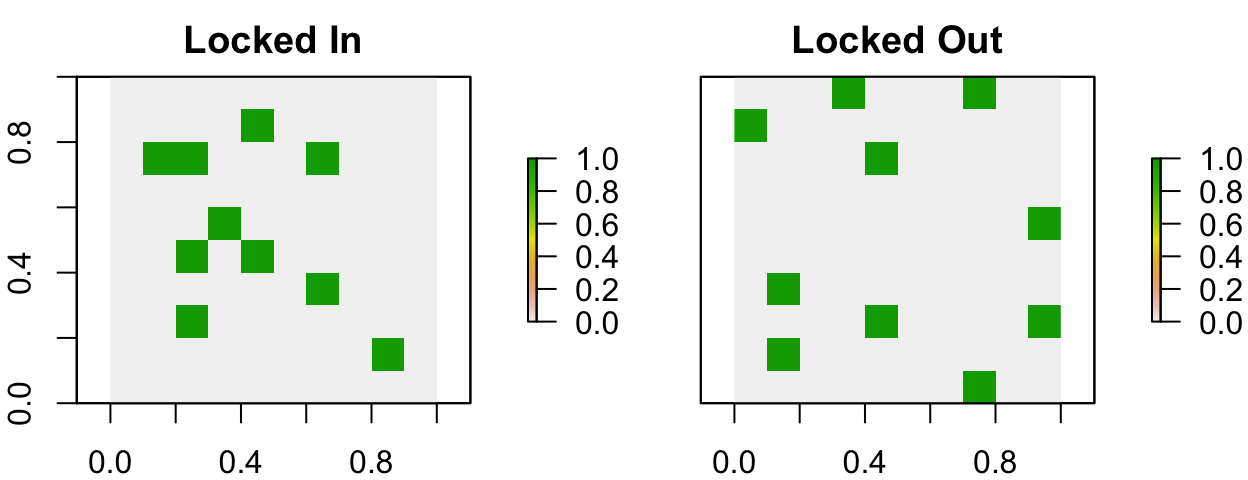
\includegraphics{SpatialPlanning_Workshop2021_files/figure-latex/unnamed-chunk-29-1} \end{center}

\begin{Shaded}
\begin{Highlighting}[]
\CommentTok{\# create a problem using raster planning unit data and use the locked raster}
\CommentTok{\# data to lock in some planning units and lock out some other planning units}
\NormalTok{p19 }\OtherTok{\textless{}{-}} \FunctionTok{problem}\NormalTok{(sim\_pu\_raster, sim\_features) }\SpecialCharTok{\%\textgreater{}\%}
       \FunctionTok{add\_min\_set\_objective}\NormalTok{() }\SpecialCharTok{\%\textgreater{}\%}
       \FunctionTok{add\_relative\_targets}\NormalTok{(}\FloatTok{0.1}\NormalTok{) }\SpecialCharTok{\%\textgreater{}\%}
       \FunctionTok{add\_locked\_in\_constraints}\NormalTok{(sim\_locked\_in\_raster) }\SpecialCharTok{\%\textgreater{}\%}
       \FunctionTok{add\_locked\_out\_constraints}\NormalTok{(sim\_locked\_out\_raster)}

\CommentTok{\# print problem}
\FunctionTok{print}\NormalTok{(p19)}
\end{Highlighting}
\end{Shaded}

\begin{verbatim}
## Conservation Problem
##   planning units: RasterLayer (90 units)
##   cost:           min: 190.13276, max: 215.86384
##   features:       layer.1, layer.2, layer.3, ... (5 features)
##   objective:      Minimum set objective 
##   targets:        Relative targets [targets (min: 0.1, max: 0.1)]
##   decisions:      default
##   constraints:    <Locked in planning units [10 locked units]
##                    Locked out planning units [10 locked units]>
##   penalties:      <none>
##   portfolio:      default
##   solver:         default
\end{verbatim}

If our planning unit data are in a spatial vector format (similar to the \texttt{sim\_pu\_polygons} data) or a tabular format (similar to \texttt{pu\_dat}), we can use the field names in the data to refer to which planning units should be locked in and / or out. For example, the \texttt{sim\_pu\_polygons} object has \texttt{TRUE} / \texttt{FALSE} values in the ``locked\_in'' field which indicate which planning units should be selected in the solution. We could use the data in this field to specify that those planning units with \texttt{TRUE} values should be locked in using the following methods.

\begin{Shaded}
\begin{Highlighting}[]
\CommentTok{\# preview first six rows of the attribute table for sim\_pu\_polygons}
\FunctionTok{head}\NormalTok{(sim\_pu\_polygons}\SpecialCharTok{@}\NormalTok{data)}
\end{Highlighting}
\end{Shaded}

\begin{verbatim}
##       cost locked_in locked_out
## 1 215.8638     FALSE      FALSE
## 2 212.7823     FALSE      FALSE
## 3 207.4962     FALSE      FALSE
## 4 208.9322     FALSE       TRUE
## 5 214.0419     FALSE      FALSE
## 6 213.7636     FALSE      FALSE
\end{verbatim}

\begin{Shaded}
\begin{Highlighting}[]
\CommentTok{\# specify locked in data using the field name}
\NormalTok{p20 }\OtherTok{\textless{}{-}} \FunctionTok{problem}\NormalTok{(sim\_pu\_polygons, sim\_features, }\AttributeTok{cost\_column =} \StringTok{"cost"}\NormalTok{) }\SpecialCharTok{\%\textgreater{}\%}
       \FunctionTok{add\_min\_set\_objective}\NormalTok{() }\SpecialCharTok{\%\textgreater{}\%}
       \FunctionTok{add\_relative\_targets}\NormalTok{(}\FloatTok{0.1}\NormalTok{) }\SpecialCharTok{\%\textgreater{}\%}
       \FunctionTok{add\_locked\_in\_constraints}\NormalTok{(}\StringTok{"locked\_in"}\NormalTok{)}

\CommentTok{\# print problem}
\FunctionTok{print}\NormalTok{(p20)}
\end{Highlighting}
\end{Shaded}

\begin{verbatim}
## Conservation Problem
##   planning units: SpatialPolygonsDataFrame (90 units)
##   cost:           min: 190.13276, max: 215.86384
##   features:       layer.1, layer.2, layer.3, ... (5 features)
##   objective:      Minimum set objective 
##   targets:        Relative targets [targets (min: 0.1, max: 0.1)]
##   decisions:      default
##   constraints:    <Locked in planning units [10 locked units]>
##   penalties:      <none>
##   portfolio:      default
##   solver:         default
\end{verbatim}

\begin{Shaded}
\begin{Highlighting}[]
\CommentTok{\# specify locked in data using the values in the field}
\NormalTok{p21 }\OtherTok{\textless{}{-}} \FunctionTok{problem}\NormalTok{(sim\_pu\_polygons, sim\_features, }\AttributeTok{cost\_column =} \StringTok{"cost"}\NormalTok{) }\SpecialCharTok{\%\textgreater{}\%}
       \FunctionTok{add\_min\_set\_objective}\NormalTok{() }\SpecialCharTok{\%\textgreater{}\%}
       \FunctionTok{add\_relative\_targets}\NormalTok{(}\FloatTok{0.1}\NormalTok{) }\SpecialCharTok{\%\textgreater{}\%}
       \FunctionTok{add\_locked\_in\_constraints}\NormalTok{(}\FunctionTok{which}\NormalTok{(sim\_pu\_polygons}\SpecialCharTok{$}\NormalTok{locked\_in))}

\CommentTok{\# print problem}
\FunctionTok{print}\NormalTok{(p21)}
\end{Highlighting}
\end{Shaded}

\begin{verbatim}
## Conservation Problem
##   planning units: SpatialPolygonsDataFrame (90 units)
##   cost:           min: 190.13276, max: 215.86384
##   features:       layer.1, layer.2, layer.3, ... (5 features)
##   objective:      Minimum set objective 
##   targets:        Relative targets [targets (min: 0.1, max: 0.1)]
##   decisions:      default
##   constraints:    <Locked in planning units [10 locked units]>
##   penalties:      <none>
##   portfolio:      default
##   solver:         default
\end{verbatim}

\hypertarget{add-penalties}{%
\subsection{Add penalties}\label{add-penalties}}

We can also add penalties to a problem to favor or penalize solutions according to a secondary objective.

Unlike the constraint functions, these functions will add extra information to the objective function of the optimization function to penalize solutions that do not exhibit specific characteristics. For example, penalties can be added to a problem to avoid highly fragmented solutions at the expense of accepting slightly more expensive solutions. All penalty functions have a \texttt{penalty} argument that controls the relative importance of the secondary penalty function compared to the primary objective function. It is worth noting that incredibly low or incredibly high \texttt{penalty} values---relative to the main objective function---can cause problems or take a very long time to solve, so when trying out a range of different penalty values it can be helpful to limit the solver to run for a set period of time.

The \emph{prioritizr R} package currently offers only two methods for adding penalties to a conservation planning problem.

\begin{itemize}
\tightlist
\item
  \textbf{Boundary penalties}: Add penalties to penalize solutions that are excessively fragmented. These penalties are similar to those used in \emph{Marxan} \citep{r3, r1}.
\end{itemize}

\begin{Shaded}
\begin{Highlighting}[]
\CommentTok{\# create problem with penalties that penalize fragmented solutions with a}
\CommentTok{\# penalty factor of 0.01}
\NormalTok{p22 }\OtherTok{\textless{}{-}} \FunctionTok{problem}\NormalTok{(sim\_pu\_raster, sim\_features) }\SpecialCharTok{\%\textgreater{}\%}
       \FunctionTok{add\_min\_set\_objective}\NormalTok{() }\SpecialCharTok{\%\textgreater{}\%}
       \FunctionTok{add\_relative\_targets}\NormalTok{(}\FloatTok{0.1}\NormalTok{) }\SpecialCharTok{\%\textgreater{}\%}
       \FunctionTok{add\_boundary\_penalties}\NormalTok{(}\AttributeTok{penalty =} \FloatTok{0.01}\NormalTok{)}

\CommentTok{\# print problem}
\FunctionTok{print}\NormalTok{(p22)}
\end{Highlighting}
\end{Shaded}

\begin{verbatim}
## Conservation Problem
##   planning units: RasterLayer (90 units)
##   cost:           min: 190.13276, max: 215.86384
##   features:       layer.1, layer.2, layer.3, ... (5 features)
##   objective:      Minimum set objective 
##   targets:        Relative targets [targets (min: 0.1, max: 0.1)]
##   decisions:      default
##   constraints:    <none>
##   penalties:      <Boundary penalties [edge factor (min: 0.5, max: 0.5), penalty (0.01), zones]>
##   portfolio:      default
##   solver:         default
\end{verbatim}

\begin{itemize}
\tightlist
\item
  \textbf{Connectivity penalties}: Add penalties to favor solutions that select combinations of planning units with high connectivity between them. These penalties are similar to those used in \emph{Marxan with Zones} \citep{r2, r1}. This function supports both symmetric and asymmetric connectivities among planning units.
\end{itemize}

\begin{Shaded}
\begin{Highlighting}[]
\CommentTok{\# create problem with penalties that favor combinations of planning units with}
\CommentTok{\# high connectivity, here we will use only the first four layers in}
\CommentTok{\# sim\_features for the features and we will use the fifth layer in sim\_features}
\CommentTok{\# to represent the connectivity data, where the connectivity\_matrix function}
\CommentTok{\# will create a matrix showing the average strength of connectivity between}
\CommentTok{\# adjacent planning units using the data in the fifth layer of sim\_features}
\NormalTok{p23 }\OtherTok{\textless{}{-}} \FunctionTok{problem}\NormalTok{(sim\_pu\_raster, sim\_features[[}\DecValTok{1}\SpecialCharTok{:}\DecValTok{4}\NormalTok{]]) }\SpecialCharTok{\%\textgreater{}\%}
       \FunctionTok{add\_min\_set\_objective}\NormalTok{() }\SpecialCharTok{\%\textgreater{}\%}
       \FunctionTok{add\_relative\_targets}\NormalTok{(}\FloatTok{0.1}\NormalTok{) }\SpecialCharTok{\%\textgreater{}\%}
       \FunctionTok{add\_boundary\_penalties}\NormalTok{(}\AttributeTok{penalty =} \DecValTok{5}\NormalTok{,}
                              \AttributeTok{data =} \FunctionTok{connectivity\_matrix}\NormalTok{(sim\_pu\_raster,}
\NormalTok{                                                         sim\_features[[}\DecValTok{5}\NormalTok{]]))}

\CommentTok{\# print problem}
\FunctionTok{print}\NormalTok{(p23)}
\end{Highlighting}
\end{Shaded}

\begin{verbatim}
## Conservation Problem
##   planning units: RasterLayer (90 units)
##   cost:           min: 190.13276, max: 215.86384
##   features:       layer.1, layer.2, layer.3, layer.4 (4 features)
##   objective:      Minimum set objective 
##   targets:        Relative targets [targets (min: 0.1, max: 0.1)]
##   decisions:      default
##   constraints:    <none>
##   penalties:      <Boundary penalties [edge factor (min: 0.5, max: 0.5), penalty (5), zones]>
##   portfolio:      default
##   solver:         default
\end{verbatim}

\begin{itemize}
\tightlist
\item
  \textbf{Linear penalties}: Add penalties to penalize solutions that select planning units according to a certain variable (e.g.~anthropogenic pressure).
\end{itemize}

\begin{Shaded}
\begin{Highlighting}[]
\CommentTok{\# create data for penalizing planning units}
\NormalTok{pen\_raster }\OtherTok{\textless{}{-}} \FunctionTok{simulate\_cost}\NormalTok{(sim\_pu\_raster)}

\CommentTok{\# create problem with penalties that penalize solutions that select}
\CommentTok{\# planning units with high values in the pen\_raster object,}
\CommentTok{\# here we will use a penalty value of 5 to indicate the trade{-}off (scaling)}
\CommentTok{\# between the penalty values (in the sim\_pu\_raster) and the main objective}
\CommentTok{\# (i.e. the cost of the solution)}
\NormalTok{p24 }\OtherTok{\textless{}{-}} \FunctionTok{problem}\NormalTok{(sim\_pu\_raster, sim\_features) }\SpecialCharTok{\%\textgreater{}\%}
       \FunctionTok{add\_min\_set\_objective}\NormalTok{() }\SpecialCharTok{\%\textgreater{}\%}
       \FunctionTok{add\_relative\_targets}\NormalTok{(}\FloatTok{0.1}\NormalTok{) }\SpecialCharTok{\%\textgreater{}\%}
       \FunctionTok{add\_linear\_penalties}\NormalTok{(}\AttributeTok{penalty =} \DecValTok{5}\NormalTok{, }\AttributeTok{data =}\NormalTok{ pen\_raster)}

\CommentTok{\# print problem}
\FunctionTok{print}\NormalTok{(p24)}
\end{Highlighting}
\end{Shaded}

\begin{verbatim}
## Conservation Problem
##   planning units: RasterLayer (90 units)
##   cost:           min: 190.13276, max: 215.86384
##   features:       layer.1, layer.2, layer.3, ... (5 features)
##   objective:      Minimum set objective 
##   targets:        Relative targets [targets (min: 0.1, max: 0.1)]
##   decisions:      default
##   constraints:    <none>
##   penalties:      <Linear penalties [penalty (5)]>
##   portfolio:      default
##   solver:         default
\end{verbatim}

\hypertarget{add-the-decision-types}{%
\subsection{Add the decision types}\label{add-the-decision-types}}

Conservation planning problems involve making decisions on how planning units will be managed.

These decisions are then associated with management actions (e.g.~turning a planning unit into a protected area). The type of decision describes how the action is applied to planning units. For instance, the default decision-type is a binary decision type, meaning that we are either selecting or not selecting planning units for management.

The \emph{prioritizr R} package currently offers the following types of decisions for customizing problems.

\begin{itemize}
\tightlist
\item
  \textbf{Binary decisions}: Add a binary decision to a conservation planning problem. This is the classic decision of either prioritizing or not prioritizing a planning unit. Typically, this decision has the assumed action of buying the planning unit to include in a protected area network. If no decision is added to a problem object, then this decision class will be used by default.
\end{itemize}

\begin{Shaded}
\begin{Highlighting}[]
\CommentTok{\# add binary decisions to a problem}
\NormalTok{p25 }\OtherTok{\textless{}{-}} \FunctionTok{problem}\NormalTok{(sim\_pu\_raster, sim\_features) }\SpecialCharTok{\%\textgreater{}\%}
       \FunctionTok{add\_min\_set\_objective}\NormalTok{() }\SpecialCharTok{\%\textgreater{}\%}
       \FunctionTok{add\_relative\_targets}\NormalTok{(}\FloatTok{0.1}\NormalTok{) }\SpecialCharTok{\%\textgreater{}\%}
       \FunctionTok{add\_binary\_decisions}\NormalTok{()}

\CommentTok{\# print problem}
\FunctionTok{print}\NormalTok{(p25)}
\end{Highlighting}
\end{Shaded}

\begin{verbatim}
## Conservation Problem
##   planning units: RasterLayer (90 units)
##   cost:           min: 190.13276, max: 215.86384
##   features:       layer.1, layer.2, layer.3, ... (5 features)
##   objective:      Minimum set objective 
##   targets:        Relative targets [targets (min: 0.1, max: 0.1)]
##   decisions:      Binary decision 
##   constraints:    <none>
##   penalties:      <none>
##   portfolio:      default
##   solver:         default
\end{verbatim}

\begin{itemize}
\tightlist
\item
  \textbf{Proportion decisions}: Add a proportion decision to a problem. This is a relaxed decision where a part of a planning unit can be prioritized, as opposed to the default of the entire planning unit. Typically, this decision has the assumed action of buying a fraction of a planning unit to include in a protected area network. Generally, problems can be solved much faster with proportion-type decisions than binary-type decisions, so they can be very useful when commercial solvers are not available.
\end{itemize}

\begin{Shaded}
\begin{Highlighting}[]
\CommentTok{\# add proportion decisions to a problem}
\NormalTok{p26 }\OtherTok{\textless{}{-}} \FunctionTok{problem}\NormalTok{(sim\_pu\_raster, sim\_features) }\SpecialCharTok{\%\textgreater{}\%}
       \FunctionTok{add\_min\_set\_objective}\NormalTok{() }\SpecialCharTok{\%\textgreater{}\%}
       \FunctionTok{add\_relative\_targets}\NormalTok{(}\FloatTok{0.1}\NormalTok{) }\SpecialCharTok{\%\textgreater{}\%}
       \FunctionTok{add\_proportion\_decisions}\NormalTok{()}

\CommentTok{\# print problem}
\FunctionTok{print}\NormalTok{(p26)}
\end{Highlighting}
\end{Shaded}

\begin{verbatim}
## Conservation Problem
##   planning units: RasterLayer (90 units)
##   cost:           min: 190.13276, max: 215.86384
##   features:       layer.1, layer.2, layer.3, ... (5 features)
##   objective:      Minimum set objective 
##   targets:        Relative targets [targets (min: 0.1, max: 0.1)]
##   decisions:      Proportion decision 
##   constraints:    <none>
##   penalties:      <none>
##   portfolio:      default
##   solver:         default
\end{verbatim}

\begin{itemize}
\tightlist
\item
  \textbf{Semi-continuous decisions}: Add a semi-continuous decision to a problem. This decision is similar to proportion decisions except that it has an upper bound parameter. By default, the decision can range from prioritizing none (0\%) to all (100\%) of a planning unit. However, a upper bound can be specified to ensure that at most only a fraction (e.g.~80\%) of a planning unit can be purchased. This type of decision may be useful when it is not practical to conserve the entire area indicated by a planning unit.
\end{itemize}

\begin{Shaded}
\begin{Highlighting}[]
\CommentTok{\# add semi{-}continuous decisions to a problem, where we can only manage at most}
\CommentTok{\# 50 \% of the area encompassed by a planning unit}
\NormalTok{p27 }\OtherTok{\textless{}{-}} \FunctionTok{problem}\NormalTok{(sim\_pu\_raster, sim\_features) }\SpecialCharTok{\%\textgreater{}\%}
       \FunctionTok{add\_min\_set\_objective}\NormalTok{() }\SpecialCharTok{\%\textgreater{}\%}
       \FunctionTok{add\_relative\_targets}\NormalTok{(}\FloatTok{0.1}\NormalTok{) }\SpecialCharTok{\%\textgreater{}\%}
       \FunctionTok{add\_semicontinuous\_decisions}\NormalTok{(}\FloatTok{0.5}\NormalTok{)}

\CommentTok{\# print problem}
\FunctionTok{print}\NormalTok{(p27)}
\end{Highlighting}
\end{Shaded}

\begin{verbatim}
## Conservation Problem
##   planning units: RasterLayer (90 units)
##   cost:           min: 190.13276, max: 215.86384
##   features:       layer.1, layer.2, layer.3, ... (5 features)
##   objective:      Minimum set objective 
##   targets:        Relative targets [targets (min: 0.1, max: 0.1)]
##   decisions:      Semicontinuous decision [upper limit (0.5)]
##   constraints:    <none>
##   penalties:      <none>
##   portfolio:      default
##   solver:         default
\end{verbatim}

\hypertarget{add-a-solver}{%
\subsection{Add a solver}\label{add-a-solver}}

Next, after specifying the mathematical formulation that underpins your conservation planning problem, you can specify how the problem should be solved. If you do not specify this information, the \emph{prioritizr R} package will automatically use the best solver currently installed on your system with some reasonable defaults. \textbf{We strongly recommend installing the \href{https://www.gurobi.com/}{Gurobi software suite and the \emph{gurobi} \emph{R} package} to solve problems, and for more information on this topic please refer to the \href{gurobi_installation.html}{Gurobi Installation Guide}}.

Currently, the \emph{prioritizr R} package only supports three different solvers.

\begin{itemize}
\tightlist
\item
  \textbf{\emph{Gurobi} solver}: \href{https://www.gurobi.com/}{\emph{Gurobi}} is a state of the art commercial optimization software. It is by far the fastest of the solvers that can be used to solve conservation problems. However, it is not freely available. That said, special licenses are available to academics at no cost.
\end{itemize}

\begin{Shaded}
\begin{Highlighting}[]
\CommentTok{\# create a problem and specify that Gurobi should be used to solve the problem}
\CommentTok{\# and specify an optimality gap of zero to obtain the optimal solution}
\NormalTok{p28 }\OtherTok{\textless{}{-}} \FunctionTok{problem}\NormalTok{(sim\_pu\_raster, sim\_features) }\SpecialCharTok{\%\textgreater{}\%}
       \FunctionTok{add\_min\_set\_objective}\NormalTok{() }\SpecialCharTok{\%\textgreater{}\%}
       \FunctionTok{add\_relative\_targets}\NormalTok{(}\FloatTok{0.1}\NormalTok{) }\SpecialCharTok{\%\textgreater{}\%}
       \FunctionTok{add\_binary\_decisions}\NormalTok{() }\SpecialCharTok{\%\textgreater{}\%}
       \FunctionTok{add\_gurobi\_solver}\NormalTok{(}\AttributeTok{gap =} \DecValTok{0}\NormalTok{)}

\CommentTok{\# print problem}
\FunctionTok{print}\NormalTok{(p28)}
\end{Highlighting}
\end{Shaded}

\begin{verbatim}
## Conservation Problem
##   planning units: RasterLayer (90 units)
##   cost:           min: 190.13276, max: 215.86384
##   features:       layer.1, layer.2, layer.3, ... (5 features)
##   objective:      Minimum set objective 
##   targets:        Relative targets [targets (min: 0.1, max: 0.1)]
##   decisions:      Binary decision 
##   constraints:    <none>
##   penalties:      <none>
##   portfolio:      default
##   solver:         Gurobi [first_feasible (0), gap (0), numeric_focus (0), presolve (2), threads (1), time_limit (2147483647), verbose (1)]
\end{verbatim}

\begin{itemize}
\tightlist
\item
  \textbf{\emph{IBM CPLEX} solver}: \href{https://www.ibm.com/analytics/cplex-optimizer}{\emph{IBM CPLEX}} is a commercial optimization software. It is faster than the open source solvers available for generating prioritizations (see below), however, it is not freely available. Similar to the \emph{Gurobi} software, special licenses are available to academics at no cost.
\end{itemize}

\begin{Shaded}
\begin{Highlighting}[]
\CommentTok{\# create a problem and specify that IBM CPLEX should be used to solve the}
\CommentTok{\# problem and specify an optimality gap of zero to obtain the optimal solution}
\CommentTok{\# p29 \textless{}{-} problem(sim\_pu\_raster, sim\_features) \%\textgreater{}\%}
\CommentTok{\#        add\_min\_set\_objective() \%\textgreater{}\%}
\CommentTok{\#        add\_relative\_targets(0.1) \%\textgreater{}\%}
\CommentTok{\#        add\_binary\_decisions() \%\textgreater{}\%}
\CommentTok{\#        add\_cplex\_solver(gap = 0)}
\CommentTok{\# }
\CommentTok{\# \# print problem}
\CommentTok{\# print(p29)}
\end{Highlighting}
\end{Shaded}

\begin{itemize}
\tightlist
\item
  \textbf{\emph{Rsymphony} solver}: \href{https://projects.coin-or.org/SYMPHONY}{\emph{SYMPHONY}} is an open-source integer programming solver that is part of the Computational Infrastructure for Operations Research (COIN-OR) project, an initiative to promote development of open-source tools for operations research. The \emph{Rsymphony R} package provides an interface to COIN-OR and is available on The Comprehensive R Archive Network (CRAN).
\end{itemize}

\begin{Shaded}
\begin{Highlighting}[]
\CommentTok{\# create a problem and specify that Rsymphony should be used to solve the}
\CommentTok{\# problem and specify an optimality gap of zero to obtain the optimal solution}
\CommentTok{\# p30 \textless{}{-} problem(sim\_pu\_raster, sim\_features) \%\textgreater{}\%}
\CommentTok{\#        add\_min\_set\_objective() \%\textgreater{}\%}
\CommentTok{\#        add\_relative\_targets(0.1) \%\textgreater{}\%}
\CommentTok{\#        add\_binary\_decisions() \%\textgreater{}\%}
\CommentTok{\#        add\_rsymphony\_solver(gap = 0)}
\CommentTok{\# }
\CommentTok{\# \# print problem}
\CommentTok{\# print(p30)}
\end{Highlighting}
\end{Shaded}

\begin{itemize}
\tightlist
\item
  \textbf{\emph{lpsymphony} solver}: The \emph{lpsymphony R} package provides a different interface to the COIN-OR software suite. This package may be easier to install on Windows and Mac OSX operating systems than the \emph{Rsymphony R} package. Unlike the \emph{Rsymphony R} package, the \emph{lpsymphony R} package is distributed through \href{http://bioconductor.org/packages/release/bioc/html/lpsymphony.html}{Bioconductor}.
\end{itemize}

\begin{Shaded}
\begin{Highlighting}[]
\CommentTok{\# create a problem and specify that lpsymphony should be used to solve the}
\CommentTok{\# problem and specify an optimality gap of zero to obtain the optimal solution}
\NormalTok{p31 }\OtherTok{\textless{}{-}} \FunctionTok{problem}\NormalTok{(sim\_pu\_raster, sim\_features) }\SpecialCharTok{\%\textgreater{}\%}
       \FunctionTok{add\_min\_set\_objective}\NormalTok{() }\SpecialCharTok{\%\textgreater{}\%}
       \FunctionTok{add\_relative\_targets}\NormalTok{(}\FloatTok{0.1}\NormalTok{) }\SpecialCharTok{\%\textgreater{}\%}
       \FunctionTok{add\_binary\_decisions}\NormalTok{() }\SpecialCharTok{\%\textgreater{}\%}
       \FunctionTok{add\_lpsymphony\_solver}\NormalTok{(}\AttributeTok{gap =} \DecValTok{0}\NormalTok{)}

\CommentTok{\# print problem}
\FunctionTok{print}\NormalTok{(p31)}
\end{Highlighting}
\end{Shaded}

\begin{verbatim}
## Conservation Problem
##   planning units: RasterLayer (90 units)
##   cost:           min: 190.13276, max: 215.86384
##   features:       layer.1, layer.2, layer.3, ... (5 features)
##   objective:      Minimum set objective 
##   targets:        Relative targets [targets (min: 0.1, max: 0.1)]
##   decisions:      Binary decision 
##   constraints:    <none>
##   penalties:      <none>
##   portfolio:      default
##   solver:         Lpsymphony [first_feasible (0), gap (0), time_limit (-1), verbose (1)]
\end{verbatim}

\hypertarget{add-a-portfolio}{%
\subsection{Add a portfolio}\label{add-a-portfolio}}

Many conservation planning exercises require a portfolio of solutions. For example, real-world exercises can involve presenting decision makers with a range of near-optimal decisions. Additionally, the number of times that different planning units are selected in different solutions can provide insight into their relative importance.

The following methods are available for generating a portfolio of solutions.

\begin{itemize}
\tightlist
\item
  \textbf{Extra portfolio}: Generate a portfolio of solutions by storing feasible solutions found during the optimization process. Note that this method requires that the \emph{Gurobi} optimization software is used to generate solutions.
\end{itemize}

\begin{Shaded}
\begin{Highlighting}[]
\CommentTok{\# create a problem and specify that a portfolio should be created using}
\CommentTok{\# extra solutions found while solving the problem}
\NormalTok{p32 }\OtherTok{\textless{}{-}} \FunctionTok{problem}\NormalTok{(sim\_pu\_raster, sim\_features) }\SpecialCharTok{\%\textgreater{}\%}
       \FunctionTok{add\_min\_set\_objective}\NormalTok{() }\SpecialCharTok{\%\textgreater{}\%}
       \FunctionTok{add\_relative\_targets}\NormalTok{(}\FloatTok{0.1}\NormalTok{) }\SpecialCharTok{\%\textgreater{}\%}
       \FunctionTok{add\_binary\_decisions}\NormalTok{() }\SpecialCharTok{\%\textgreater{}\%}
       \FunctionTok{add\_extra\_portfolio}\NormalTok{()}

\CommentTok{\# print problem}
\FunctionTok{print}\NormalTok{(p32)}
\end{Highlighting}
\end{Shaded}

\begin{verbatim}
## Conservation Problem
##   planning units: RasterLayer (90 units)
##   cost:           min: 190.13276, max: 215.86384
##   features:       layer.1, layer.2, layer.3, ... (5 features)
##   objective:      Minimum set objective 
##   targets:        Relative targets [targets (min: 0.1, max: 0.1)]
##   decisions:      Binary decision 
##   constraints:    <none>
##   penalties:      <none>
##   portfolio:      Extra portfolio
##   solver:         default
\end{verbatim}

\begin{itemize}
\tightlist
\item
  \textbf{Top portfolio}: Generate a portfolio of solutions by finding a pre-specified number of solutions that are closest to optimality (i.e the top solutions). Note that this method requires that the \emph{Gurobi} optimization software is used to generate solutions.
\end{itemize}

\begin{Shaded}
\begin{Highlighting}[]
\CommentTok{\# create a problem and specify that a portfolio should be created using}
\CommentTok{\# the top five solutions}
\NormalTok{p33 }\OtherTok{\textless{}{-}} \FunctionTok{problem}\NormalTok{(sim\_pu\_raster, sim\_features) }\SpecialCharTok{\%\textgreater{}\%}
       \FunctionTok{add\_min\_set\_objective}\NormalTok{() }\SpecialCharTok{\%\textgreater{}\%}
       \FunctionTok{add\_relative\_targets}\NormalTok{(}\FloatTok{0.1}\NormalTok{) }\SpecialCharTok{\%\textgreater{}\%}
       \FunctionTok{add\_binary\_decisions}\NormalTok{() }\SpecialCharTok{\%\textgreater{}\%}
       \FunctionTok{add\_top\_portfolio}\NormalTok{(}\AttributeTok{number\_solutions =} \DecValTok{5}\NormalTok{)}

\CommentTok{\# print problem}
\FunctionTok{print}\NormalTok{(p33)}
\end{Highlighting}
\end{Shaded}

\begin{verbatim}
## Conservation Problem
##   planning units: RasterLayer (90 units)
##   cost:           min: 190.13276, max: 215.86384
##   features:       layer.1, layer.2, layer.3, ... (5 features)
##   objective:      Minimum set objective 
##   targets:        Relative targets [targets (min: 0.1, max: 0.1)]
##   decisions:      Binary decision 
##   constraints:    <none>
##   penalties:      <none>
##   portfolio:      Top portfolio [number_solutions (5)]
##   solver:         default
\end{verbatim}

\begin{itemize}
\tightlist
\item
  \textbf{Gap portfolio}: Generate a portfolio of solutions by finding a certain number of solutions that are all within a pre-specified optimality gap. This method is especially useful for generating multiple solutions that can used be to calculate selection frequencies (similar to \emph{Marxan}). Note that this method requires that the \emph{Gurobi} optimization software is used to generate solutions.
\end{itemize}

\begin{Shaded}
\begin{Highlighting}[]
\CommentTok{\# create a problem and specify that a portfolio should be created by}
\CommentTok{\# finding five solutions within 10\% of optimality}
\NormalTok{p34 }\OtherTok{\textless{}{-}} \FunctionTok{problem}\NormalTok{(sim\_pu\_raster, sim\_features) }\SpecialCharTok{\%\textgreater{}\%}
       \FunctionTok{add\_min\_set\_objective}\NormalTok{() }\SpecialCharTok{\%\textgreater{}\%}
       \FunctionTok{add\_relative\_targets}\NormalTok{(}\FloatTok{0.1}\NormalTok{) }\SpecialCharTok{\%\textgreater{}\%}
       \FunctionTok{add\_binary\_decisions}\NormalTok{() }\SpecialCharTok{\%\textgreater{}\%}
       \FunctionTok{add\_gap\_portfolio}\NormalTok{(}\AttributeTok{number\_solutions =} \DecValTok{5}\NormalTok{, }\AttributeTok{pool\_gap =} \FloatTok{0.2}\NormalTok{)}

\CommentTok{\# print problem}
\FunctionTok{print}\NormalTok{(p34)}
\end{Highlighting}
\end{Shaded}

\begin{verbatim}
## Conservation Problem
##   planning units: RasterLayer (90 units)
##   cost:           min: 190.13276, max: 215.86384
##   features:       layer.1, layer.2, layer.3, ... (5 features)
##   objective:      Minimum set objective 
##   targets:        Relative targets [targets (min: 0.1, max: 0.1)]
##   decisions:      Binary decision 
##   constraints:    <none>
##   penalties:      <none>
##   portfolio:      Gap portfolio [number_solutions (5), pool_gap (0.2)]
##   solver:         default
\end{verbatim}

\begin{itemize}
\tightlist
\item
  \textbf{Cuts portfolio}: Generate a portfolio of distinct solutions within a pre-specified optimality gap. This method is only recommended if the \emph{Gurobi} optimization solver is not available.
\end{itemize}

\begin{Shaded}
\begin{Highlighting}[]
\CommentTok{\# create a problem and specify that a portfolio containing 10 solutions}
\CommentTok{\# should be created using using Bender\textquotesingle{}s cuts}
\NormalTok{p35 }\OtherTok{\textless{}{-}} \FunctionTok{problem}\NormalTok{(sim\_pu\_raster, sim\_features) }\SpecialCharTok{\%\textgreater{}\%}
  \FunctionTok{add\_min\_set\_objective}\NormalTok{() }\SpecialCharTok{\%\textgreater{}\%}
  \FunctionTok{add\_relative\_targets}\NormalTok{(}\FloatTok{0.1}\NormalTok{) }\SpecialCharTok{\%\textgreater{}\%}
  \FunctionTok{add\_binary\_decisions}\NormalTok{() }\SpecialCharTok{\%\textgreater{}\%}
  \FunctionTok{add\_cuts\_portfolio}\NormalTok{(}\AttributeTok{number\_solutions =} \DecValTok{10}\NormalTok{)}

\CommentTok{\# print problem}
\FunctionTok{print}\NormalTok{(p35)}
\end{Highlighting}
\end{Shaded}

\begin{verbatim}
## Conservation Problem
##   planning units: RasterLayer (90 units)
##   cost:           min: 190.13276, max: 215.86384
##   features:       layer.1, layer.2, layer.3, ... (5 features)
##   objective:      Minimum set objective 
##   targets:        Relative targets [targets (min: 0.1, max: 0.1)]
##   decisions:      Binary decision 
##   constraints:    <none>
##   penalties:      <none>
##   portfolio:      Cuts portfolio [number_solutions (10)]
##   solver:         default
\end{verbatim}

\begin{itemize}
\tightlist
\item
  \textbf{Shuffle portfolio}: Generate a portfolio of solutions by randomly reordering the data prior to attempting to solve the problem. If the \emph{Gurobi} optimization solver is not available, this method is the fastest method for generating a set number of solutions within a specified distance from optimality.
\end{itemize}

\begin{Shaded}
\begin{Highlighting}[]
\CommentTok{\# create a problem and specify a portfolio should be created that contains}
\CommentTok{\# 10 solutions and that any duplicate solutions should not be removed}
\NormalTok{p36 }\OtherTok{\textless{}{-}} \FunctionTok{problem}\NormalTok{(sim\_pu\_raster, sim\_features) }\SpecialCharTok{\%\textgreater{}\%}
  \FunctionTok{add\_min\_set\_objective}\NormalTok{() }\SpecialCharTok{\%\textgreater{}\%}
  \FunctionTok{add\_relative\_targets}\NormalTok{(}\FloatTok{0.1}\NormalTok{) }\SpecialCharTok{\%\textgreater{}\%}
  \FunctionTok{add\_binary\_decisions}\NormalTok{() }\SpecialCharTok{\%\textgreater{}\%}
  \FunctionTok{add\_shuffle\_portfolio}\NormalTok{(}\AttributeTok{number\_solutions =} \DecValTok{10}\NormalTok{, }\AttributeTok{remove\_duplicates =} \ConstantTok{FALSE}\NormalTok{)}

\CommentTok{\# print problem}
\FunctionTok{print}\NormalTok{(p36)}
\end{Highlighting}
\end{Shaded}

\begin{verbatim}
## Conservation Problem
##   planning units: RasterLayer (90 units)
##   cost:           min: 190.13276, max: 215.86384
##   features:       layer.1, layer.2, layer.3, ... (5 features)
##   objective:      Minimum set objective 
##   targets:        Relative targets [targets (min: 0.1, max: 0.1)]
##   decisions:      Binary decision 
##   constraints:    <none>
##   penalties:      <none>
##   portfolio:      Shuffle portfolio [number_solutions (10), remove_duplicates (0), threads (1)]
##   solver:         default
\end{verbatim}

\hypertarget{solve-the-problem}{%
\subsection{Solve the problem}\label{solve-the-problem}}

Finally, after formulating our conservation planning problem and specifying how the problem should be solved, we can use the \texttt{solve} function to obtain a solution. Note that the solver will typically print out some information describing the size of the problem and report its progress when searching for a suitable solution.

\begin{Shaded}
\begin{Highlighting}[]
\CommentTok{\# formulate the problem}
\NormalTok{p37 }\OtherTok{\textless{}{-}} \FunctionTok{problem}\NormalTok{(sim\_pu\_raster, sim\_features) }\SpecialCharTok{\%\textgreater{}\%}
  \FunctionTok{add\_min\_set\_objective}\NormalTok{() }\SpecialCharTok{\%\textgreater{}\%}
  \FunctionTok{add\_relative\_targets}\NormalTok{(}\FloatTok{0.1}\NormalTok{) }\SpecialCharTok{\%\textgreater{}\%}
  \FunctionTok{add\_boundary\_penalties}\NormalTok{(}\AttributeTok{penalty =} \DecValTok{500}\NormalTok{, }\AttributeTok{edge\_factor =} \FloatTok{0.5}\NormalTok{) }\SpecialCharTok{\%\textgreater{}\%}
  \FunctionTok{add\_binary\_decisions}\NormalTok{()}

\CommentTok{\# solve the problem (using the default solver)}
\NormalTok{s37 }\OtherTok{\textless{}{-}} \FunctionTok{solve}\NormalTok{(p37)}
\end{Highlighting}
\end{Shaded}

\begin{verbatim}
## Gurobi Optimizer version 9.1.1 build v9.1.1rc0 (mac64)
## Thread count: 4 physical cores, 8 logical processors, using up to 1 threads
## Optimize a model with 293 rows, 234 columns and 1026 nonzeros
## Model fingerprint: 0xbd38144b
## Variable types: 0 continuous, 234 integer (234 binary)
## Coefficient statistics:
##   Matrix range     [2e-01, 1e+00]
##   Objective range  [1e+02, 4e+02]
##   Bounds range     [1e+00, 1e+00]
##   RHS range        [3e+00, 8e+00]
## Found heuristic solution: objective 20287.196992
## Found heuristic solution: objective 3087.9617505
## Presolve time: 0.00s
## Presolved: 293 rows, 234 columns, 1026 nonzeros
## Variable types: 0 continuous, 234 integer (234 binary)
## Presolved: 293 rows, 234 columns, 1026 nonzeros
## 
## 
## Root relaxation: objective 2.265862e+03, 218 iterations, 0.01 seconds
## 
##     Nodes    |    Current Node    |     Objective Bounds      |     Work
##  Expl Unexpl |  Obj  Depth IntInf | Incumbent    BestBd   Gap | It/Node Time
## 
##      0     0 2265.86242    0  234 3087.96175 2265.86242  26.6%     -    0s
## H    0     0                    2920.9854189 2265.86242  22.4%     -    0s
##      0     0 2327.26806    0  232 2920.98542 2327.26806  20.3%     -    0s
##      0     0 2368.37316    0  226 2920.98542 2368.37316  18.9%     -    0s
##      0     0 2376.91951    0  223 2920.98542 2376.91951  18.6%     -    0s
##      0     0 2376.91951    0  223 2920.98542 2376.91951  18.6%     -    0s
## H    0     0                    2910.0202492 2376.91951  18.3%     -    0s
## H    0     0                    2676.6543486 2376.91951  11.2%     -    0s
##      0     2 2377.44918    0  223 2676.65435 2377.44918  11.2%     -    0s
## H   27    27                    2676.6537993 2377.44918  11.2%  16.9    0s
## H   56    40                    2676.6531808 2388.87827  10.8%  16.2    0s
## 
## Cutting planes:
##   Gomory: 3
## 
## Explored 57 nodes (1397 simplex iterations) in 0.16 seconds
## Thread count was 1 (of 8 available processors)
## 
## Solution count 5: 2676.65 2910.02 2920.99 ... 20287.2
## 
## Optimal solution found (tolerance 1.00e-01)
## Best objective 2.676653180861e+03, best bound 2.413625263266e+03, gap 9.8267%
\end{verbatim}

\begin{Shaded}
\begin{Highlighting}[]
\CommentTok{\# plot solution}
\FunctionTok{plot}\NormalTok{(s37, }\AttributeTok{col =} \FunctionTok{c}\NormalTok{(}\StringTok{"grey90"}\NormalTok{, }\StringTok{"darkgreen"}\NormalTok{), }\AttributeTok{main =} \StringTok{"Solution"}\NormalTok{,}
     \AttributeTok{xlim =} \FunctionTok{c}\NormalTok{(}\SpecialCharTok{{-}}\FloatTok{0.1}\NormalTok{, }\FloatTok{1.1}\NormalTok{), }\AttributeTok{ylim =} \FunctionTok{c}\NormalTok{(}\SpecialCharTok{{-}}\FloatTok{0.1}\NormalTok{, }\FloatTok{1.1}\NormalTok{))}
\end{Highlighting}
\end{Shaded}

\begin{center}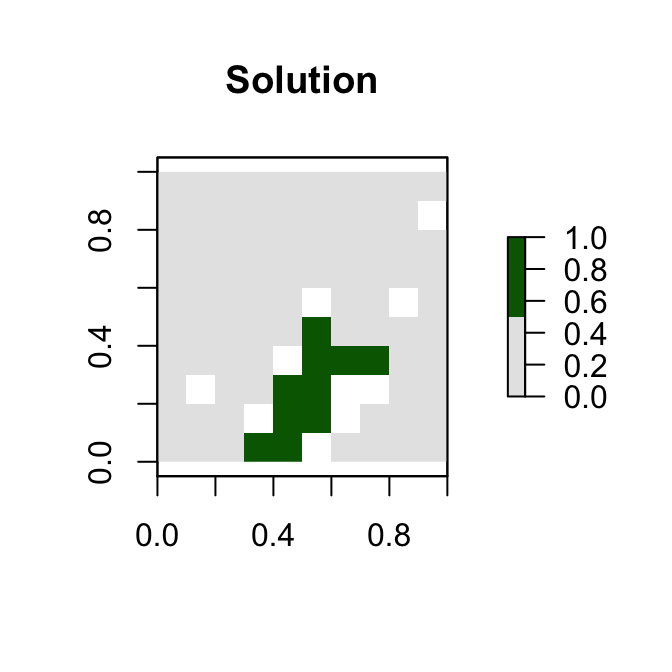
\includegraphics{SpatialPlanning_Workshop2021_files/figure-latex/unnamed-chunk-46-1} \end{center}

We can plot this solution because the planning unit input data are spatially referenced in a raster format. The output format will always match the planning unit data used to initialize the problem. For example, the solution to a problem with planning units in a spatial vector (shapefile) format would also be in a spatial vector format. Similarly, if the planning units were in a tabular format (i.e.~\texttt{data.frame}), the solution would also be returned in a tabular format.

We can also extract attributes from the solution that describe the quality of the solution and the optimization process.

\begin{Shaded}
\begin{Highlighting}[]
\CommentTok{\# extract the objective (numerical value being minimized or maximized)}
\FunctionTok{print}\NormalTok{(}\FunctionTok{attr}\NormalTok{(s37, }\StringTok{"objective"}\NormalTok{))}
\end{Highlighting}
\end{Shaded}

\begin{verbatim}
## solution_1 
##   2676.653
\end{verbatim}

\begin{Shaded}
\begin{Highlighting}[]
\CommentTok{\# extract time spent solving solution}
\FunctionTok{print}\NormalTok{(}\FunctionTok{attr}\NormalTok{(s37, }\StringTok{"runtime"}\NormalTok{))}
\end{Highlighting}
\end{Shaded}

\begin{verbatim}
## solution_1 
##  0.1554909
\end{verbatim}

\begin{Shaded}
\begin{Highlighting}[]
\CommentTok{\# extract state message from the solver that describes why this specific}
\CommentTok{\# solution was returned}
\FunctionTok{print}\NormalTok{(}\FunctionTok{attr}\NormalTok{(s37, }\StringTok{"status"}\NormalTok{))}
\end{Highlighting}
\end{Shaded}

\begin{verbatim}
## solution_1 
##  "OPTIMAL"
\end{verbatim}

\hypertarget{evaluate-the-performance-of-a-solution}{%
\subsection{Evaluate the performance of a solution}\label{evaluate-the-performance-of-a-solution}}

After obtaining a solution to a conservation planning problem, it can be useful to calculate various summary statistics to understand its performance. The following functions are available to summarize a solution:

\begin{itemize}
\tightlist
\item
  Calculate the number of planning units selected within a solution.
\end{itemize}

\begin{Shaded}
\begin{Highlighting}[]
\CommentTok{\# calculate statistic}
\FunctionTok{eval\_n\_summary}\NormalTok{(p37, s37)}
\end{Highlighting}
\end{Shaded}

\begin{verbatim}
## # A tibble: 1 x 2
##   summary  cost
##   <chr>   <dbl>
## 1 overall    10
\end{verbatim}

\begin{itemize}
\tightlist
\item
  Calculate the total cost of a solution.
\end{itemize}

\begin{Shaded}
\begin{Highlighting}[]
\CommentTok{\# calculate statistic}
\FunctionTok{eval\_cost\_summary}\NormalTok{(p37, s37)}
\end{Highlighting}
\end{Shaded}

\begin{verbatim}
## # A tibble: 1 x 2
##   summary  cost
##   <chr>   <dbl>
## 1 overall 2002.
\end{verbatim}

\begin{itemize}
\tightlist
\item
  Calculate how well features are represented by a solution. This function can be used for problems that are built using targets and those that are not built using targets.
\end{itemize}

\begin{Shaded}
\begin{Highlighting}[]
\CommentTok{\# calculate statistics}
\FunctionTok{eval\_feature\_representation\_summary}\NormalTok{(p37, s37)}
\end{Highlighting}
\end{Shaded}

\begin{verbatim}
## # A tibble: 5 x 5
##   summary feature total_amount absolute_held relative_held
##   <chr>   <chr>          <dbl>         <dbl>         <dbl>
## 1 overall layer.1         83.3          8.96         0.108
## 2 overall layer.2         31.2          3.19         0.102
## 3 overall layer.3         72.0          7.56         0.105
## 4 overall layer.4         42.7          4.32         0.101
## 5 overall layer.5         56.7          5.93         0.105
\end{verbatim}

\begin{itemize}
\tightlist
\item
  Calculate how well feature representation targets are met by a solution. This function can only be used with problems containing targets.
\end{itemize}

\begin{Shaded}
\begin{Highlighting}[]
\CommentTok{\# calculate statistics}
\FunctionTok{eval\_target\_coverage\_summary}\NormalTok{(p37, s37, }\AttributeTok{include\_zone =} \ConstantTok{FALSE}\NormalTok{, }\AttributeTok{include\_sense =} \ConstantTok{FALSE}\NormalTok{)}
\end{Highlighting}
\end{Shaded}

\begin{verbatim}
## # A tibble: 5 x 9
##   feature met   total_amount absolute_target absolute_held absolute_shortfall
##   <chr>   <lgl>        <dbl>           <dbl>         <dbl>              <dbl>
## 1 layer.1 TRUE          83.3            8.33          8.96                  0
## 2 layer.2 TRUE          31.2            3.12          3.19                  0
## 3 layer.3 TRUE          72.0            7.20          7.56                  0
## 4 layer.4 TRUE          42.7            4.27          4.32                  0
## 5 layer.5 TRUE          56.7            5.67          5.93                  0
##   relative_target relative_held relative_shortfall
##             <dbl>         <dbl>              <dbl>
## 1             0.1         0.108                  0
## 2             0.1         0.102                  0
## 3             0.1         0.105                  0
## 4             0.1         0.101                  0
## 5             0.1         0.105                  0
\end{verbatim}

\begin{itemize}
\tightlist
\item
  Calculate the exposed boundary length (perimeter) associated with a solution.
\end{itemize}

\begin{Shaded}
\begin{Highlighting}[]
\CommentTok{\# calculate statistic}
\FunctionTok{eval\_boundary\_summary}\NormalTok{(p37, s37)}
\end{Highlighting}
\end{Shaded}

\begin{verbatim}
## # A tibble: 1 x 2
##   summary boundary
##   <chr>      <dbl>
## 1 overall     1.35
\end{verbatim}

\begin{itemize}
\tightlist
\item
  Calculate the connectivity held within a solution.
\end{itemize}

\begin{Shaded}
\begin{Highlighting}[]
\CommentTok{\# calculate statistic}
\CommentTok{\# here we use the raster data for the first feature as an example}
\CommentTok{\# to parametrize pair{-}wise connectivity between different planning units}
\FunctionTok{eval\_connectivity\_summary}\NormalTok{(}
\NormalTok{  p37, s37, }\AttributeTok{data =} \FunctionTok{connectivity\_matrix}\NormalTok{(sim\_pu\_raster, sim\_features[[}\DecValTok{1}\NormalTok{]]))}
\end{Highlighting}
\end{Shaded}

\begin{verbatim}
## # A tibble: 1 x 2
##   summary connectivity
##   <chr>          <dbl>
## 1 overall         1.80
\end{verbatim}

\hypertarget{importance-irreplaceability}{%
\subsection{Importance (irreplaceability)}\label{importance-irreplaceability}}

Conservation plans can take a long time to implement. Since funding availability and habitat quality can decline over time, \textbf{it is critical that the most important places in a prioritization are scheduled for protection as early as possible}. For instance,\\
* some planning units in a solution might contain many rare species which do not occur in any other planning units.
* some planning units might offer an especially high return on investment that reduces costs considerably.

As a consequence, conservation planners often need information on which planning units selected in a prioritization are most important to the overall success of the prioritization. To achieve this, conservation planners can use importance (irreplaceability) scores for each planning unit selected in a solution.

The \emph{prioritizr R} package offers multiple methods for assessing importance. These includes scores calculated based on:

\begin{itemize}
\item
  \textbf{Replacement Costs}: {[}\texttt{eval\_replacement\_importance()}; \citet{r31}{]} quantify the change in the objective function (e.g.~additional costs required to meet feature targets) of the optimal solution if a given planning unit in a solution cannot be acquired. They can:

  \begin{enumerate}
  \def\labelenumi{\arabic{enumi}.}
  \tightlist
  \item
    account for the cost of different planning units,\\
  \item
    account for multiple management zones,
  \item
    apply to any objective function, and
  \item
    identify truly irreplaceable planning units (denoted with infinite values).
  \end{enumerate}
\item
  \textbf{Ferrier Scores}: {[}\texttt{eval\_ferrier\_importance()}; \citet{r34}{]} quantify the importance of planning units for meeting feature targets. They can only be applied to conservation problems with a minimum set objective and a single zone (i.e.~the classic \emph{Marxan}-type problem). Furthermore---unlike the replacement cost scores---the Ferrier scores provide a score for each feature within each planning unit, providing insight into why certain planning units are more important than other planning units.
\item
  \textbf{rarity weighted richness scores} {[}\texttt{eval\_rare\_richness\_importance()}; \citet{r33}{]} are simply a measure of biological diversity. They do not account for planning costs, multiple management zones, objective functions, or feature targets (or weightings). They merely describe the spatial patterns of biodiversity, and do not account for many of the factors needed to quantify the importance of a planning unit for achieving conservation goals.
\end{itemize}

We recommend using replacement cost scores for small and moderate sized problems (e.g.~less than 30,000 planning units) when it is feasible to do so. It can take a very long time to compute replacement cost scores, and so it is simply not feasible to compute these scores for particularly large problems. For moderate and large sized problems (e.g.~more than 30,000 planning units), we recommend using the rarity weighted richness scores. Beware, it has been known for decades that such static measures of biodiversity lead to poor conservation plans \citep{r17}. Although the Ferrier method is also provided, we do not recommend using this method until it has been verified by a statistical expert.

Below we will generate a solution, and then calculate importance scores for the planning units selected in the solution using the three different methods.

\begin{Shaded}
\begin{Highlighting}[]
\CommentTok{\# formulate the problem}
\NormalTok{p38 }\OtherTok{\textless{}{-}} \FunctionTok{problem}\NormalTok{(sim\_pu\_raster, sim\_features) }\SpecialCharTok{\%\textgreater{}\%}
  \FunctionTok{add\_min\_set\_objective}\NormalTok{() }\SpecialCharTok{\%\textgreater{}\%}
  \FunctionTok{add\_relative\_targets}\NormalTok{(}\FloatTok{0.1}\NormalTok{) }\SpecialCharTok{\%\textgreater{}\%}
  \FunctionTok{add\_binary\_decisions}\NormalTok{()}

\CommentTok{\# solve the problem}
\NormalTok{s38 }\OtherTok{\textless{}{-}} \FunctionTok{solve}\NormalTok{(p38)}
\end{Highlighting}
\end{Shaded}

\begin{verbatim}
## Gurobi Optimizer version 9.1.1 build v9.1.1rc0 (mac64)
## Thread count: 4 physical cores, 8 logical processors, using up to 1 threads
## Optimize a model with 5 rows, 90 columns and 450 nonzeros
## Model fingerprint: 0x6442bf6e
## Variable types: 0 continuous, 90 integer (90 binary)
## Coefficient statistics:
##   Matrix range     [2e-01, 9e-01]
##   Objective range  [2e+02, 2e+02]
##   Bounds range     [1e+00, 1e+00]
##   RHS range        [3e+00, 8e+00]
## Found heuristic solution: objective 2337.9617505
## Presolve time: 0.00s
## Presolved: 5 rows, 90 columns, 450 nonzeros
## Variable types: 0 continuous, 90 integer (90 binary)
## Presolved: 5 rows, 90 columns, 450 nonzeros
## 
## 
## Root relaxation: objective 1.931582e+03, 12 iterations, 0.00 seconds
## 
##     Nodes    |    Current Node    |     Objective Bounds      |     Work
##  Expl Unexpl |  Obj  Depth IntInf | Incumbent    BestBd   Gap | It/Node Time
## 
##      0     0 1931.58191    0    4 2337.96175 1931.58191  17.4%     -    0s
## H    0     0                    1987.3985265 1931.58191  2.81%     -    0s
## 
## Explored 1 nodes (12 simplex iterations) in 0.00 seconds
## Thread count was 1 (of 8 available processors)
## 
## Solution count 2: 1987.4 2337.96 
## 
## Optimal solution found (tolerance 1.00e-01)
## Best objective 1.987398526526e+03, best bound 1.931581908865e+03, gap 2.8085%
\end{verbatim}

\begin{Shaded}
\begin{Highlighting}[]
\CommentTok{\# plot solution}
\FunctionTok{plot}\NormalTok{(s38, }\AttributeTok{col =} \FunctionTok{c}\NormalTok{(}\StringTok{"grey90"}\NormalTok{, }\StringTok{"darkgreen"}\NormalTok{), }\AttributeTok{main =} \StringTok{"Solution"}\NormalTok{,}
     \AttributeTok{xlim =} \FunctionTok{c}\NormalTok{(}\SpecialCharTok{{-}}\FloatTok{0.1}\NormalTok{, }\FloatTok{1.1}\NormalTok{), }\AttributeTok{ylim =} \FunctionTok{c}\NormalTok{(}\SpecialCharTok{{-}}\FloatTok{0.1}\NormalTok{, }\FloatTok{1.1}\NormalTok{))}
\end{Highlighting}
\end{Shaded}

\begin{center}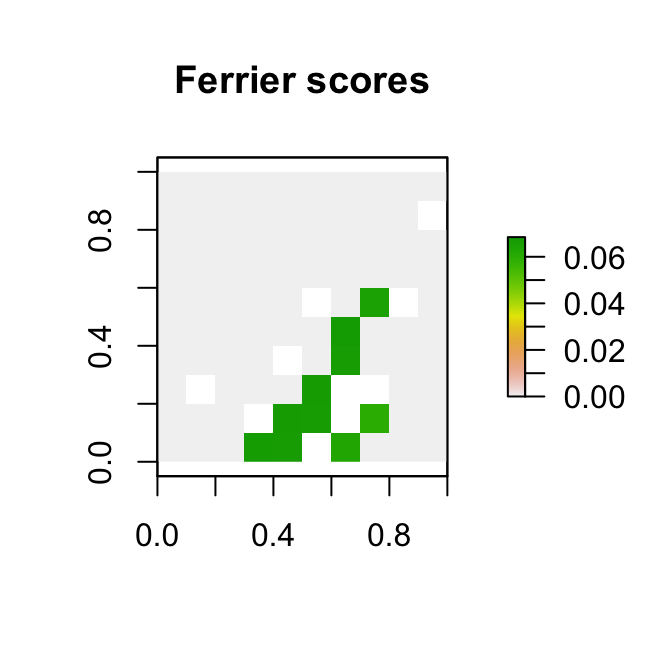
\includegraphics{SpatialPlanning_Workshop2021_files/figure-latex/unnamed-chunk-54-1} \end{center}

\begin{Shaded}
\begin{Highlighting}[]
\CommentTok{\# calculate replacement cost scores and make the solver quiet}
\NormalTok{rc38 }\OtherTok{\textless{}{-}}\NormalTok{ p38 }\SpecialCharTok{\%\textgreater{}\%}
  \FunctionTok{add\_default\_solver}\NormalTok{(}\AttributeTok{gap =} \DecValTok{0}\NormalTok{, }\AttributeTok{verbose =} \ConstantTok{FALSE}\NormalTok{) }\SpecialCharTok{\%\textgreater{}\%}
  \FunctionTok{eval\_replacement\_importance}\NormalTok{(s38)}

\CommentTok{\# plot replacement cost scores}
\FunctionTok{plot}\NormalTok{(rc38, }\AttributeTok{main =} \StringTok{"replacement cost"}\NormalTok{)}
\end{Highlighting}
\end{Shaded}

\begin{center}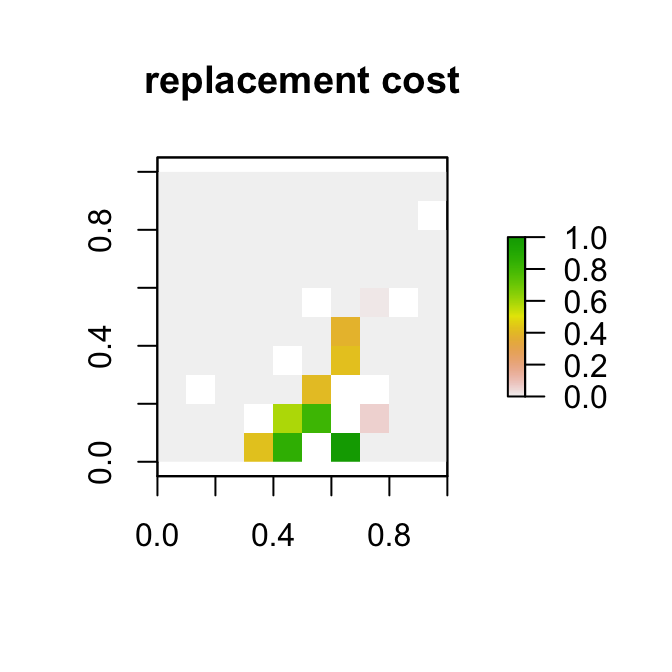
\includegraphics{SpatialPlanning_Workshop2021_files/figure-latex/unnamed-chunk-54-2} \end{center}

\begin{Shaded}
\begin{Highlighting}[]
\CommentTok{\# calculate Ferrier scores and extract total score}
\NormalTok{fs38 }\OtherTok{\textless{}{-}} \FunctionTok{eval\_ferrier\_importance}\NormalTok{(p38, s38)[[}\StringTok{"total"}\NormalTok{]]}

\CommentTok{\# plot Ferrier scores}
\FunctionTok{plot}\NormalTok{(fs38, }\AttributeTok{main =} \StringTok{"Ferrier scores"}\NormalTok{)}
\end{Highlighting}
\end{Shaded}

\begin{center}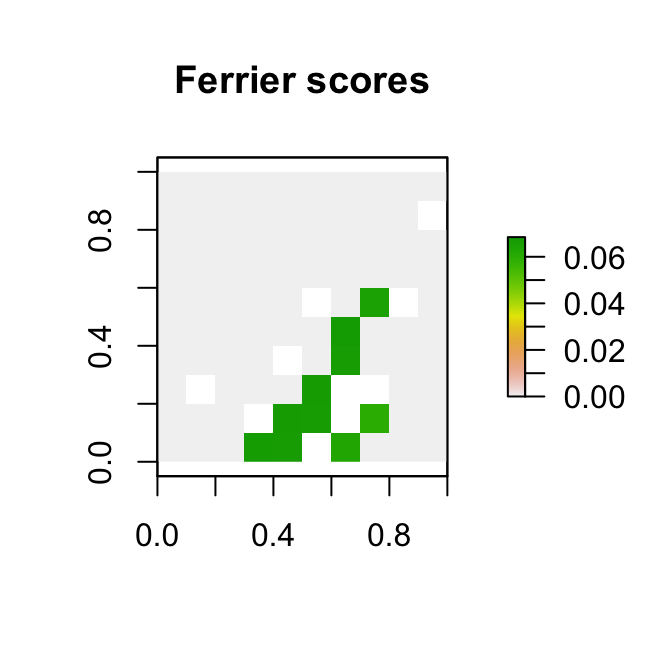
\includegraphics{SpatialPlanning_Workshop2021_files/figure-latex/unnamed-chunk-55-1} \end{center}

\begin{Shaded}
\begin{Highlighting}[]
\CommentTok{\# calculate rarity weighted richness scores}
\NormalTok{rwr38 }\OtherTok{\textless{}{-}} \FunctionTok{eval\_rare\_richness\_importance}\NormalTok{(p38, s38)}

\CommentTok{\# plot replacement cost scores}
\FunctionTok{plot}\NormalTok{(rwr38, }\AttributeTok{main =} \StringTok{"rarity weighted richness"}\NormalTok{)}
\end{Highlighting}
\end{Shaded}

\begin{center}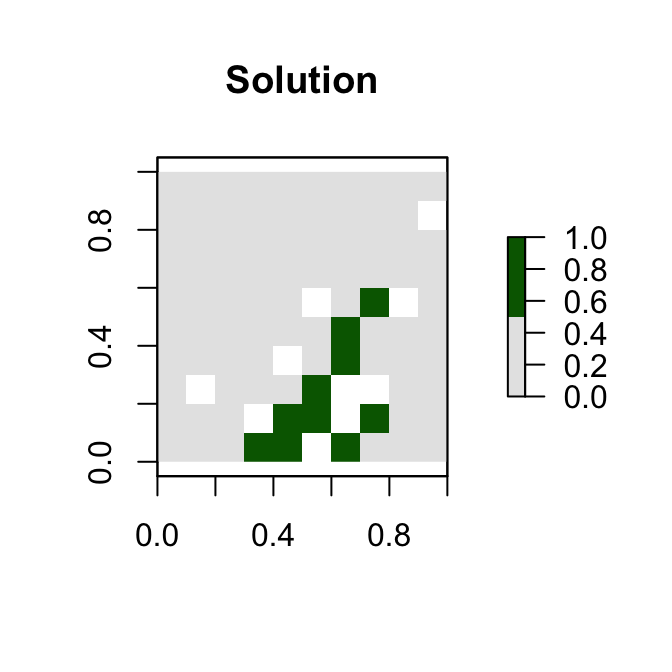
\includegraphics{SpatialPlanning_Workshop2021_files/figure-latex/unnamed-chunk-56-1} \end{center}

Although rarity weighted richness scores can approximate scores derived from the other two methods in certain conservation planning exercises, we can see that the rarity weighted richness scores provide completely different results in this case.

\hypertarget{data}{%
\chapter{Spatial Data}\label{data}}

The aim of this tutorial is to provide a worked example of how vector-based data can be used to develop conservation prioritizations using the \emph{prioritizr R} package. The dataset used in this tutorial was originally a subset of a larger spatial prioritization project performed under contract to Australia's Department of Environment and Water Resources \citep{r30}.

This dataset contains two items.

\begin{itemize}
\item
  First, a spatial planning unit layer that has an attribute table which contains three columns: integer unique identifiers (``id''), unimproved land values (``cost''), and their existing level of protection (``status''). Units with 50 \% or more of their area contained in protected areas are associated with a status of 2, otherwise they are associated with a value of 0.
\item
  The second item in this dataset is the raster-based feature data. Specifically, the feature data is expressed as a stack of rasters (termed a \texttt{RasterStack} object). Here each layer in the stack represents the distribution of a different vegetation class in Tasmania, Australia. There are 62 vegetation classes in total. For a given layer, pixel values indicate the presence (value of 1) or absence (value of 0) of the vegetation class in an area.
\end{itemize}

First, load the required packages and the data.

\hypertarget{data-import}{%
\section{Data import}\label{data-import}}

\begin{Shaded}
\begin{Highlighting}[]
\CommentTok{\# load packages}
\FunctionTok{library}\NormalTok{(prioritizr)}
\FunctionTok{library}\NormalTok{(prioritizrdata)}
\FunctionTok{library}\NormalTok{(sf)}
\FunctionTok{library}\NormalTok{(rgdal)}
\FunctionTok{library}\NormalTok{(raster)}
\FunctionTok{library}\NormalTok{(rgeos)}
\FunctionTok{library}\NormalTok{(mapview)}
\FunctionTok{library}\NormalTok{(units)}
\FunctionTok{library}\NormalTok{(scales)}
\FunctionTok{library}\NormalTok{(assertthat)}
\FunctionTok{library}\NormalTok{(gridExtra)}
\FunctionTok{library}\NormalTok{(dplyr)}
\end{Highlighting}
\end{Shaded}

\begin{Shaded}
\begin{Highlighting}[]
\DocumentationTok{\#\# Some of this data is built in to the Prioritizr package, but it is lower resolution so we use that in the data/ folder.}
\CommentTok{\# load planning unit data}
\CommentTok{\# data(tas\_pu) \# SpatialPolygonsDataFrame \# If raw, use readOGR(filename)}

\CommentTok{\# load conservation feature data}
\CommentTok{\# data(tas\_features) \# RasterStack \# If raw, use stack(filename)}

\NormalTok{albers }\OtherTok{\textless{}{-}} \StringTok{"+proj=aea +lat\_1={-}18 +lat\_2={-}36 +lat\_0=0 +lon\_0=132 +x\_0=0 +y\_0=0 +ellps=GRS80 +towgs84=0,0,0,0,0,0,0 +units=m +no\_defs"}

\NormalTok{tas\_pu }\OtherTok{\textless{}{-}} \FunctionTok{readOGR}\NormalTok{(}\StringTok{"data/pu.shp"}\NormalTok{)}
\end{Highlighting}
\end{Shaded}

\begin{verbatim}
## OGR data source with driver: ESRI Shapefile 
## Source: "/Users/jason/GitHub/SpatialPlanning_Workshop2021/data/pu.shp", layer: "pu"
## with 1130 features
## It has 5 fields
\end{verbatim}

\begin{Shaded}
\begin{Highlighting}[]
\NormalTok{tas\_features }\OtherTok{\textless{}{-}} \FunctionTok{stack}\NormalTok{(}\StringTok{"data/vegetation.tif"}\NormalTok{)}
\FunctionTok{proj4string}\NormalTok{(tas\_pu) }\OtherTok{\textless{}{-}}\NormalTok{ albers }\CommentTok{\# There is a problem with projection so we re{-}add it here}
\FunctionTok{proj4string}\NormalTok{(tas\_features) }\OtherTok{\textless{}{-}}\NormalTok{ albers }\CommentTok{\# There is a problem with projection so we re{-}add it here}

\NormalTok{tas\_pu}\SpecialCharTok{$}\NormalTok{locked\_out[}\DecValTok{1}\SpecialCharTok{:}\DecValTok{500}\NormalTok{] }\OtherTok{\textless{}{-}} \ConstantTok{FALSE} \CommentTok{\# There is a problem later on so we remove some of the locked out areas to improve chance of a solution}
\NormalTok{tas\_pu}\SpecialCharTok{$}\NormalTok{locked\_in }\OtherTok{\textless{}{-}} \FunctionTok{as.logical}\NormalTok{(tas\_pu}\SpecialCharTok{$}\NormalTok{locked\_in) }\CommentTok{\# Convert to logical}
\NormalTok{tas\_pu}\SpecialCharTok{$}\NormalTok{locked\_out }\OtherTok{\textless{}{-}} \FunctionTok{as.logical}\NormalTok{(tas\_pu}\SpecialCharTok{$}\NormalTok{locked\_out) }\CommentTok{\# Convert to logical}

\CommentTok{\# A function to plot the solution. }
\NormalTok{plot\_solution }\OtherTok{\textless{}{-}} \ControlFlowTok{function}\NormalTok{(s)\{}
\NormalTok{  s}\SpecialCharTok{$}\NormalTok{solution\_1 }\OtherTok{\textless{}{-}} \FunctionTok{factor}\NormalTok{(s}\SpecialCharTok{$}\NormalTok{solution\_1)}
  \FunctionTok{plot}\NormalTok{(}\FunctionTok{st\_as\_sf}\NormalTok{(s[, }\StringTok{"solution\_1"}\NormalTok{]), }\AttributeTok{pal =} \FunctionTok{c}\NormalTok{(}\StringTok{"grey90"}\NormalTok{, }\StringTok{"darkgreen"}\NormalTok{), }\AttributeTok{main =} \StringTok{"Solution 1"}\NormalTok{)}
\NormalTok{\}}

\NormalTok{tas\_sum }\OtherTok{\textless{}{-}}\NormalTok{ raster}\SpecialCharTok{::}\FunctionTok{calc}\NormalTok{(tas\_features, sum, }\AttributeTok{na.rm =} \ConstantTok{TRUE}\NormalTok{)}

\FunctionTok{plot}\NormalTok{(tas\_sum)}
\end{Highlighting}
\end{Shaded}

\begin{center}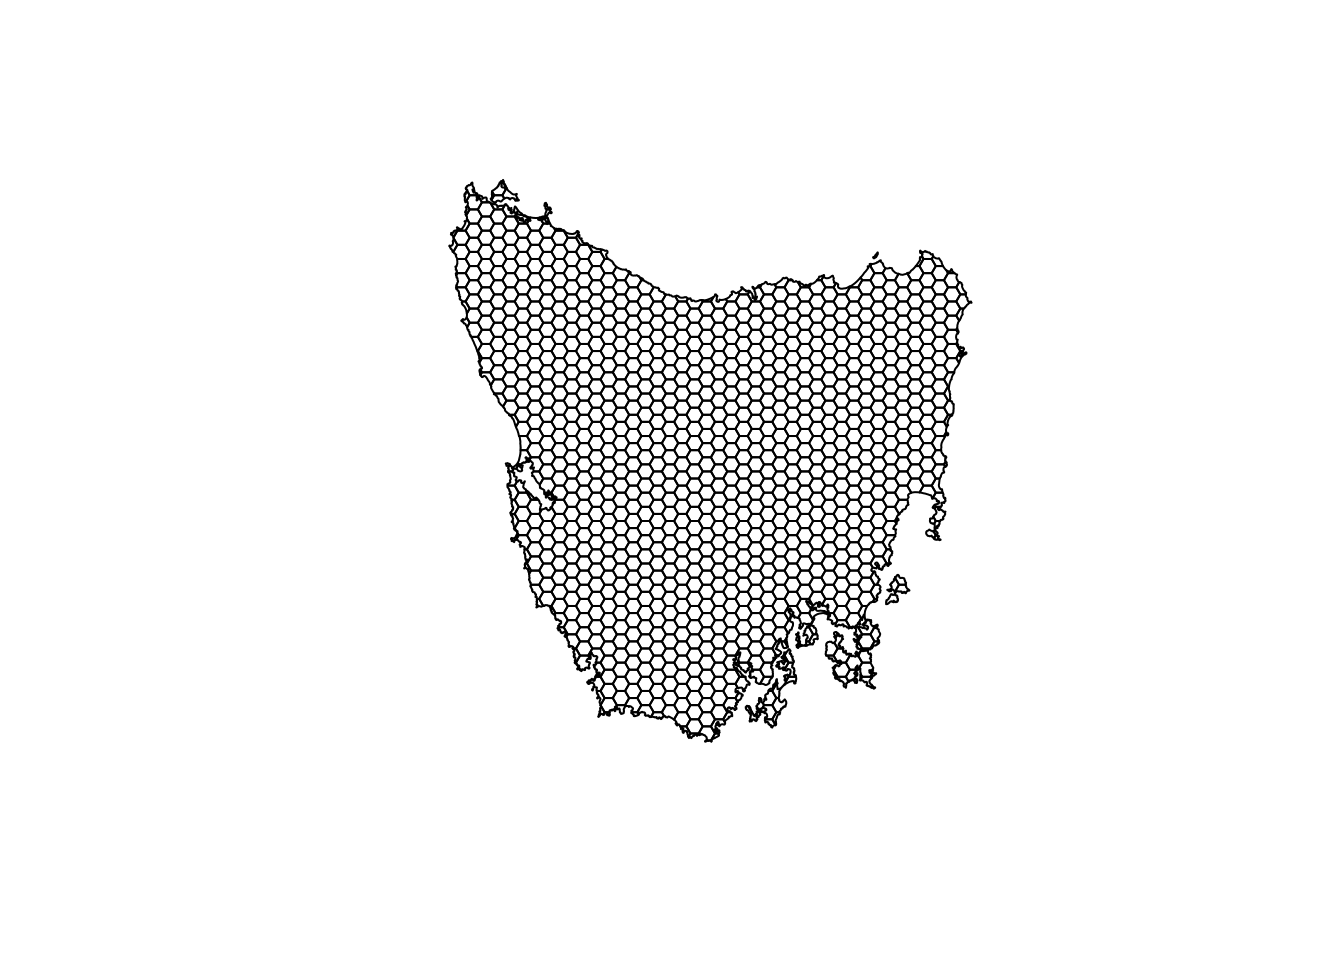
\includegraphics{SpatialPlanning_Workshop2021_files/figure-latex/unnamed-chunk-58-1} \end{center}

\clearpage

\hypertarget{planning-unit-data}{%
\section{Planning unit data}\label{planning-unit-data}}

The planning unit data contains spatial data describing the geometry for each planning unit and attribute data with information about each planning unit (e.g.~cost values). Let's investigate the \texttt{tas\_pu} object. The attribute data contains 5 columns with contain the following information:

\begin{itemize}
\tightlist
\item
  \texttt{id}: unique identifiers for each planning unit
\item
  \texttt{cost}: acquisition cost values for each planning unit (millions of Australian dollars).
\item
  \texttt{status}: status information for each planning unit (only relevant with Marxan)
\item
  \texttt{locked\_in}: logical values (i.e.~\texttt{TRUE}/\texttt{FALSE}) indicating if planning units are covered by protected areas or not.
\item
  \texttt{locked\_out}: logical values (i.e.~\texttt{TRUE}/\texttt{FALSE}) indicating if planning units cannot be managed as a protected area because they contain are too degraded.
\end{itemize}

\begin{Shaded}
\begin{Highlighting}[]
\CommentTok{\# print a short summary of the data}
\FunctionTok{print}\NormalTok{(tas\_pu)}
\end{Highlighting}
\end{Shaded}

\begin{verbatim}
## class       : SpatialPolygonsDataFrame 
## features    : 1130 
## extent      : 1080623, 1399989, -4840595, -4497092  (xmin, xmax, ymin, ymax)
## crs         : +proj=aea +lat_0=0 +lon_0=132 +lat_1=-18 +lat_2=-36 +x_0=0 +y_0=0 +ellps=GRS80 +units=m +no_defs 
## variables   : 5
## names       :   id,              cost, status, locked_in, locked_out 
## min values  :    1, 0.192488262910798,      0,         0,          0 
## max values  : 1130,  61.9272727272727,      2,         1,          1
\end{verbatim}

\begin{Shaded}
\begin{Highlighting}[]
\CommentTok{\# plot the planning unit data}
\FunctionTok{plot}\NormalTok{(tas\_pu)}
\end{Highlighting}
\end{Shaded}

\begin{center}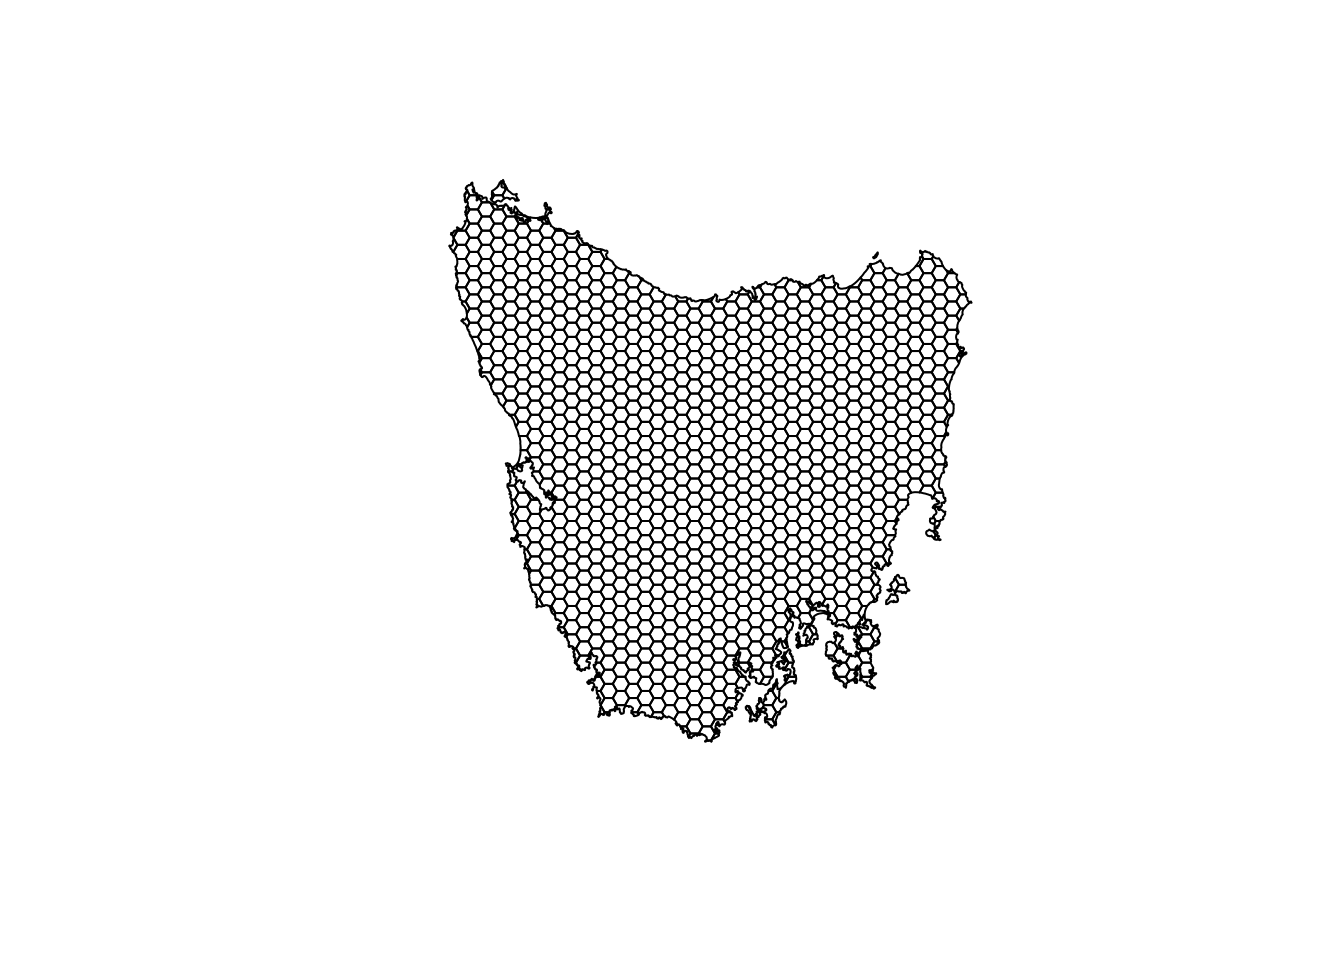
\includegraphics{SpatialPlanning_Workshop2021_files/figure-latex/unnamed-chunk-59-1} \end{center}

\begin{Shaded}
\begin{Highlighting}[]
\CommentTok{\# print the structure of object}
\FunctionTok{str}\NormalTok{(tas\_pu, }\AttributeTok{max.level =} \DecValTok{2}\NormalTok{)}
\end{Highlighting}
\end{Shaded}

\begin{verbatim}
## Formal class 'SpatialPolygonsDataFrame' [package "sp"] with 5 slots
##   ..@ data       :'data.frame':  1130 obs. of  5 variables:
##   ..@ polygons   :List of 1130
##   ..@ plotOrder  : int [1:1130] 217 973 506 645 705 975 253 271 704 889 ...
##   ..@ bbox       : num [1:2, 1:2] 1080623 -4840595 1399989 -4497092
##   .. ..- attr(*, "dimnames")=List of 2
##   ..@ proj4string:Formal class 'CRS' [package "sp"] with 1 slot
\end{verbatim}

\begin{Shaded}
\begin{Highlighting}[]
\CommentTok{\# print the class of the object}
\FunctionTok{class}\NormalTok{(tas\_pu)}
\end{Highlighting}
\end{Shaded}

\begin{verbatim}
## [1] "SpatialPolygonsDataFrame"
## attr(,"package")
## [1] "sp"
\end{verbatim}

\begin{Shaded}
\begin{Highlighting}[]
\CommentTok{\# print the slots of the object}
\FunctionTok{slotNames}\NormalTok{(tas\_pu)}
\end{Highlighting}
\end{Shaded}

\begin{verbatim}
## [1] "data"        "polygons"    "plotOrder"   "bbox"        "proj4string"
\end{verbatim}

\begin{Shaded}
\begin{Highlighting}[]
\CommentTok{\# print the geometry for the 80th planning unit}
\NormalTok{tas\_pu}\SpecialCharTok{@}\NormalTok{polygons[[}\DecValTok{80}\NormalTok{]]}
\end{Highlighting}
\end{Shaded}

\begin{verbatim}
## An object of class "Polygons"
## Slot "Polygons":
## [[1]]
## An object of class "Polygon"
## Slot "labpt":
## [1]  1289177 -4558185
## 
## Slot "area":
## [1] 1060361
## 
## Slot "hole":
## [1] FALSE
## 
## Slot "ringDir":
## [1] 1
## 
## Slot "coords":
##          [,1]     [,2]
##  [1,] 1288123 -4558431
##  [2,] 1287877 -4558005
##  [3,] 1288177 -4558019
##  [4,] 1288278 -4558054
##  [5,] 1288834 -4558038
##  [6,] 1289026 -4557929
##  [7,] 1289168 -4557928
##  [8,] 1289350 -4557790
##  [9,] 1289517 -4557744
## [10,] 1289618 -4557773
## [11,] 1289836 -4557965
## [12,] 1290000 -4557984
## [13,] 1290025 -4557987
## [14,] 1290144 -4558168
## [15,] 1290460 -4558431
## [16,] 1288123 -4558431
## 
## 
## 
## Slot "plotOrder":
## [1] 1
## 
## Slot "labpt":
## [1]  1289177 -4558185
## 
## Slot "ID":
## [1] "79"
## 
## Slot "area":
## [1] 1060361
\end{verbatim}

\begin{Shaded}
\begin{Highlighting}[]
\CommentTok{\# print the coordinate reference system}
\FunctionTok{print}\NormalTok{(tas\_pu}\SpecialCharTok{@}\NormalTok{proj4string)}
\end{Highlighting}
\end{Shaded}

\begin{verbatim}
## CRS arguments:
##  +proj=aea +lat_0=0 +lon_0=132 +lat_1=-18 +lat_2=-36 +x_0=0 +y_0=0
## +ellps=GRS80 +units=m +no_defs
\end{verbatim}

\begin{Shaded}
\begin{Highlighting}[]
\CommentTok{\# print number of planning units (geometries) in the data}
\FunctionTok{nrow}\NormalTok{(tas\_pu)}
\end{Highlighting}
\end{Shaded}

\begin{verbatim}
## [1] 1130
\end{verbatim}

\begin{Shaded}
\begin{Highlighting}[]
\CommentTok{\# print the first six rows in the attribute data}
\FunctionTok{head}\NormalTok{(tas\_pu}\SpecialCharTok{@}\NormalTok{data)}
\end{Highlighting}
\end{Shaded}

\begin{verbatim}
##   id     cost status locked_in locked_out
## 0  1 60.24638      0     FALSE      FALSE
## 1  2 19.86301      0     FALSE      FALSE
## 2  3 59.68051      0     FALSE      FALSE
## 3  4 32.41614      0     FALSE      FALSE
## 4  5 26.17706      0     FALSE      FALSE
## 5  6 51.26218      0     FALSE      FALSE
\end{verbatim}

\begin{Shaded}
\begin{Highlighting}[]
\CommentTok{\# print the first six values in the cost column of the attribute data}
\FunctionTok{head}\NormalTok{(tas\_pu}\SpecialCharTok{$}\NormalTok{cost)}
\end{Highlighting}
\end{Shaded}

\begin{verbatim}
## [1] 60.24638 19.86301 59.68051 32.41614 26.17706 51.26218
\end{verbatim}

\begin{Shaded}
\begin{Highlighting}[]
\CommentTok{\# print the highest cost value}
\FunctionTok{max}\NormalTok{(tas\_pu}\SpecialCharTok{$}\NormalTok{cost)}
\end{Highlighting}
\end{Shaded}

\begin{verbatim}
## [1] 61.92727
\end{verbatim}

\begin{Shaded}
\begin{Highlighting}[]
\CommentTok{\# print the smallest cost value}
\FunctionTok{min}\NormalTok{(tas\_pu}\SpecialCharTok{$}\NormalTok{cost)}
\end{Highlighting}
\end{Shaded}

\begin{verbatim}
## [1] 0.1924883
\end{verbatim}

\begin{Shaded}
\begin{Highlighting}[]
\CommentTok{\# print average cost value}
\FunctionTok{mean}\NormalTok{(tas\_pu}\SpecialCharTok{$}\NormalTok{cost)}
\end{Highlighting}
\end{Shaded}

\begin{verbatim}
## [1] 25.13536
\end{verbatim}

\begin{Shaded}
\begin{Highlighting}[]
\CommentTok{\# plot a map of the planning unit cost data}
\FunctionTok{spplot}\NormalTok{(tas\_pu, }\StringTok{"cost"}\NormalTok{)}
\end{Highlighting}
\end{Shaded}

\begin{center}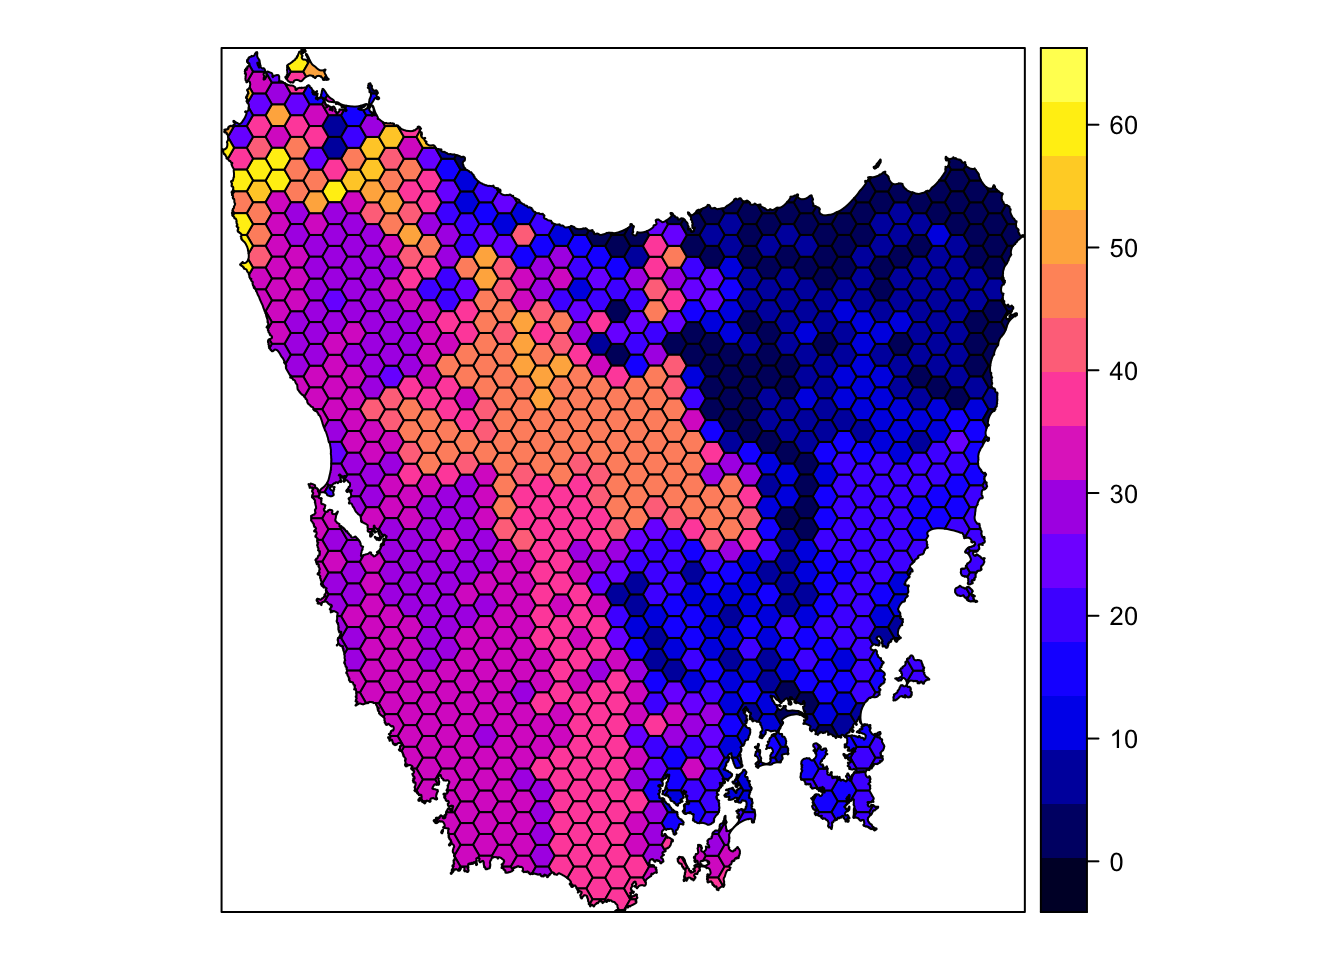
\includegraphics[width=0.6\linewidth]{SpatialPlanning_Workshop2021_files/figure-latex/unnamed-chunk-60-1} \end{center}

\begin{Shaded}
\begin{Highlighting}[]
\CommentTok{\# plot an interactive map of the planning unit cost data}
\FunctionTok{mapview}\NormalTok{(tas\_pu, }\AttributeTok{zcol =} \StringTok{"cost"}\NormalTok{)}
\end{Highlighting}
\end{Shaded}

Now, you can try and answer some questions about the planning unit data.

\begin{rmdquestion}
\begin{enumerate}
\def\labelenumi{\arabic{enumi}.}
\tightlist
\item
  How many planning units are in the planning unit data?
\item
  What is the highest cost value?
\item
  How many planning units are covered by the protected areas (hint: \texttt{sum(x)})?
\item
  What is the proportion of the planning units that are covered by the protected areas (hint: \texttt{mean(x)})?
\item
  How many planning units are highly degraded (hint: \texttt{sum(x)})?
\item
  What is the proportion of planning units are highly degraded (hint: \texttt{mean(x)})?
\item
  Can you verify that all values in the \texttt{locked\_in} and \texttt{locked\_out} columns are zero or one (hint: \texttt{min(x)} and \texttt{max(x)})?.
\item
  Can you verify that none of the planning units are missing cost values (hint: \texttt{all(is.finite(x))})?.
\item
  Can you very that none of the planning units have duplicated identifiers? (hint: \texttt{sum(duplicated(x))})?
\item
  Is there a spatial pattern in the planning unit cost values (hint: use \texttt{spplot} to make a map).
\item
  Is there a spatial pattern in where most planning units are covered by protected areas (hint: use \texttt{spplot} to make a map).
\end{enumerate}
\end{rmdquestion}

\clearpage

\hypertarget{vegetation-data}{%
\section{Vegetation data}\label{vegetation-data}}

The vegetation data describes the spatial distribution of 62 vegetation classes in the study area. This data is in a raster format and so the data are organized using a square grid comprising square grid cells that are each the same size. In our case, the raster data contains multiple layers (also called ``bands'') and each layer corresponds to a spatial grid with exactly the same area and has exactly the same dimensionality (i.e.~number of rows, columns, and cells).

In this dataset, there are 62 different regular spatial grids layered on top of each other -- with each layer corresponding to a different vegetation class -- and each of these layers contains a grid with 343 rows, 320 columns, and 109760 cells.

Within each layer, each cell corresponds to a 1 by 1 km square. The values associated with each grid cell indicate the (one) presence or (zero) absence of a given vegetation class in the cell.

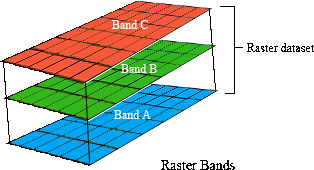
\includegraphics{images/rasterbands.png}

Let's explore the vegetation data.

\begin{Shaded}
\begin{Highlighting}[]
\CommentTok{\# print a short summary of the data}
\FunctionTok{print}\NormalTok{(tas\_features)}
\end{Highlighting}
\end{Shaded}

\begin{verbatim}
## class      : RasterStack 
## dimensions : 343, 320, 109760, 62  (nrow, ncol, ncell, nlayers)
## resolution : 1000, 1000  (x, y)
## extent     : 1080496, 1400496, -4841217, -4498217  (xmin, xmax, ymin, ymax)
## crs        : +proj=aea +lat_0=0 +lon_0=132 +lat_1=-18 +lat_2=-36 +x_0=0 +y_0=0 +ellps=GRS80 +units=m +no_defs 
## names      : vegetation.1, vegetation.2, vegetation.3, vegetation.4, vegetation.5, vegetation.6, vegetation.7, vegetation.8, vegetation.9, vegetation.10, vegetation.11, vegetation.12, vegetation.13, vegetation.14, vegetation.15, ... 
## min values :            0,            0,            0,            0,            0,            0,            0,            0,            0,             0,             0,             0,             0,             0,             0, ... 
## max values :            1,            1,            1,            1,            1,            1,            1,            1,            1,             1,             1,             1,             1,             1,             1, ...
\end{verbatim}

\begin{Shaded}
\begin{Highlighting}[]
\CommentTok{\# plot a map of the 36th vegetation class}
\FunctionTok{plot}\NormalTok{(tas\_features[[}\DecValTok{36}\NormalTok{]])}
\end{Highlighting}
\end{Shaded}

\begin{center}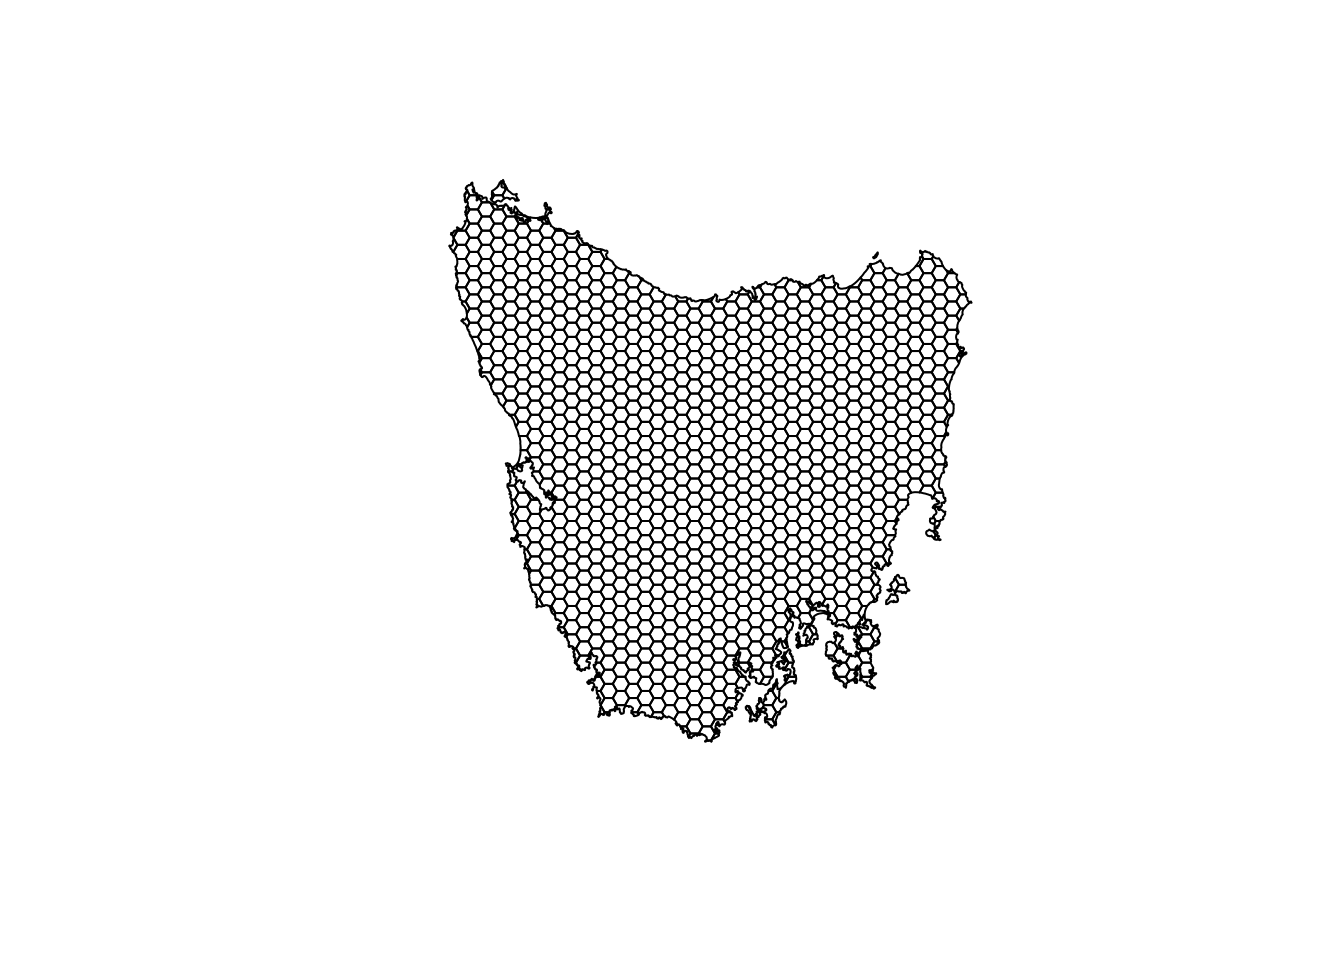
\includegraphics{SpatialPlanning_Workshop2021_files/figure-latex/unnamed-chunk-63-1} \end{center}

\begin{Shaded}
\begin{Highlighting}[]
\CommentTok{\# plot an interactive map of the 36th vegetation class}
\FunctionTok{mapview}\NormalTok{(tas\_features[[}\DecValTok{36}\NormalTok{]])}
\end{Highlighting}
\end{Shaded}

\begin{Shaded}
\begin{Highlighting}[]
\CommentTok{\# print number of rows in the data}
\FunctionTok{nrow}\NormalTok{(tas\_features)}
\end{Highlighting}
\end{Shaded}

\begin{verbatim}
## [1] 343
\end{verbatim}

\begin{Shaded}
\begin{Highlighting}[]
\CommentTok{\# print number of columns  in the data}
\FunctionTok{ncol}\NormalTok{(tas\_features)}
\end{Highlighting}
\end{Shaded}

\begin{verbatim}
## [1] 320
\end{verbatim}

\begin{Shaded}
\begin{Highlighting}[]
\CommentTok{\# print number of cells in the data}
\FunctionTok{ncell}\NormalTok{(tas\_features)}
\end{Highlighting}
\end{Shaded}

\begin{verbatim}
## [1] 109760
\end{verbatim}

\begin{Shaded}
\begin{Highlighting}[]
\CommentTok{\# print number of layers in the data}
\FunctionTok{nlayers}\NormalTok{(tas\_features)}
\end{Highlighting}
\end{Shaded}

\begin{verbatim}
## [1] 62
\end{verbatim}

\begin{Shaded}
\begin{Highlighting}[]
\CommentTok{\# print  resolution on the x{-}axis}
\FunctionTok{xres}\NormalTok{(tas\_features)}
\end{Highlighting}
\end{Shaded}

\begin{verbatim}
## [1] 1000
\end{verbatim}

\begin{Shaded}
\begin{Highlighting}[]
\CommentTok{\# print resolution on the y{-}axis}
\FunctionTok{yres}\NormalTok{(tas\_features)}
\end{Highlighting}
\end{Shaded}

\begin{verbatim}
## [1] 1000
\end{verbatim}

\begin{Shaded}
\begin{Highlighting}[]
\CommentTok{\# print spatial extent of the grid, i.e. coordinates for corners}
\FunctionTok{extent}\NormalTok{(tas\_features)}
\end{Highlighting}
\end{Shaded}

\begin{verbatim}
## class      : Extent 
## xmin       : 1080496 
## xmax       : 1400496 
## ymin       : -4841217 
## ymax       : -4498217
\end{verbatim}

\begin{Shaded}
\begin{Highlighting}[]
\CommentTok{\# print the coordinate reference system}
\FunctionTok{print}\NormalTok{(tas\_features}\SpecialCharTok{@}\NormalTok{crs)}
\end{Highlighting}
\end{Shaded}

\begin{verbatim}
## CRS arguments:
##  +proj=aea +lat_0=0 +lon_0=132 +lat_1=-18 +lat_2=-36 +x_0=0 +y_0=0
## +ellps=GRS80 +units=m +no_defs
\end{verbatim}

\begin{Shaded}
\begin{Highlighting}[]
\CommentTok{\# print a summary of the first layer in the stack}
\FunctionTok{print}\NormalTok{(tas\_features[[}\DecValTok{1}\NormalTok{]])}
\end{Highlighting}
\end{Shaded}

\begin{verbatim}
## class      : RasterLayer 
## band       : 1  (of  62  bands)
## dimensions : 343, 320, 109760  (nrow, ncol, ncell)
## resolution : 1000, 1000  (x, y)
## extent     : 1080496, 1400496, -4841217, -4498217  (xmin, xmax, ymin, ymax)
## crs        : +proj=aea +lat_0=0 +lon_0=132 +lat_1=-18 +lat_2=-36 +x_0=0 +y_0=0 +ellps=GRS80 +units=m +no_defs 
## source     : /Users/jason/GitHub/SpatialPlanning_Workshop2021/data/vegetation.tif 
## names      : vegetation.1 
## values     : 0, 1  (min, max)
\end{verbatim}

\begin{Shaded}
\begin{Highlighting}[]
\CommentTok{\# print the value in the 800th cell in the first layer of the stack}
\FunctionTok{print}\NormalTok{(tas\_features[[}\DecValTok{1}\NormalTok{]][}\DecValTok{800}\NormalTok{])}
\end{Highlighting}
\end{Shaded}

\begin{verbatim}
##   
## 0
\end{verbatim}

\begin{Shaded}
\begin{Highlighting}[]
\CommentTok{\# print the value of the cell located in the 30th row and the 60th column of}
\CommentTok{\# the first layer}
\FunctionTok{print}\NormalTok{(tas\_features[[}\DecValTok{1}\NormalTok{]][}\DecValTok{30}\NormalTok{, }\DecValTok{60}\NormalTok{])}
\end{Highlighting}
\end{Shaded}

\begin{verbatim}
##   
## 0
\end{verbatim}

\begin{Shaded}
\begin{Highlighting}[]
\CommentTok{\# calculate the sum of all the cell values in the first layer}
\FunctionTok{cellStats}\NormalTok{(tas\_features[[}\DecValTok{1}\NormalTok{]], }\StringTok{"sum"}\NormalTok{)}
\end{Highlighting}
\end{Shaded}

\begin{verbatim}
## [1] 36
\end{verbatim}

\begin{Shaded}
\begin{Highlighting}[]
\CommentTok{\# calculate the maximum value of all the cell values in the first layer}
\FunctionTok{cellStats}\NormalTok{(tas\_features[[}\DecValTok{1}\NormalTok{]], }\StringTok{"max"}\NormalTok{)}
\end{Highlighting}
\end{Shaded}

\begin{verbatim}
## [1] 1
\end{verbatim}

\begin{Shaded}
\begin{Highlighting}[]
\CommentTok{\# calculate the minimum value of all the cell values in the first layer}
\FunctionTok{cellStats}\NormalTok{(tas\_features[[}\DecValTok{1}\NormalTok{]], }\StringTok{"min"}\NormalTok{)}
\end{Highlighting}
\end{Shaded}

\begin{verbatim}
## [1] 0
\end{verbatim}

\begin{Shaded}
\begin{Highlighting}[]
\CommentTok{\# calculate the mean value of all the cell values in the first layer}
\FunctionTok{cellStats}\NormalTok{(tas\_features[[}\DecValTok{1}\NormalTok{]], }\StringTok{"mean"}\NormalTok{)}
\end{Highlighting}
\end{Shaded}

\begin{verbatim}
## [1] 0.0003279883
\end{verbatim}

\clearpage

\begin{Shaded}
\begin{Highlighting}[]
\CommentTok{\# calculate the maximum value in each layer}
\FunctionTok{as\_tibble}\NormalTok{(}\FunctionTok{data.frame}\NormalTok{(}\AttributeTok{max =} \FunctionTok{cellStats}\NormalTok{(tas\_features, }\StringTok{"max"}\NormalTok{)))}
\end{Highlighting}
\end{Shaded}

\begin{verbatim}
## # A tibble: 62 x 1
##      max
##    <dbl>
##  1     1
##  2     1
##  3     1
##  4     1
##  5     1
##  6     1
##  7     1
##  8     1
##  9     1
## 10     1
## # ... with 52 more rows
\end{verbatim}

Now, you can try and answer some questions about the vegetation data.

\begin{rmdquestion}
\begin{enumerate}
\def\labelenumi{\arabic{enumi}.}
\tightlist
\item
  What part of the study area is the 51st vegetation class found in (hint: make a map)?
\item
  What proportion of cells contain the 12th vegetation class?
\item
  Which vegetation class is present in the greatest number of cells?
\item
  The planning unit data and the vegetation data should have the same coordinate reference system. Can you check if they are the same?
\end{enumerate}
\end{rmdquestion}

\hypertarget{spatial-prioritizations}{%
\chapter{Spatial prioritizations}\label{spatial-prioritizations}}

\hypertarget{introduction-1}{%
\section{Introduction}\label{introduction-1}}

Here we will develop prioritizations to identify priority areas for protected area establishment.

\hypertarget{starting-out-simple}{%
\section{Starting out simple}\label{starting-out-simple}}

To start things off, let's keep things simple. Let's create a prioritization using the \href{https://prioritizr.net/reference/add_min_set_objective.html}{minimum set formulation of the reserve selection problem}. This formulation means that \textbf{we want a solution that will meet the targets for our biodiversity features for minimum cost}. Here, we will set 5\% targets for each vegetation class and use the data in the \texttt{cost} column to specify acquisition costs. Unlike Marxan, we do not have to calibrate species penalty factors (SPFs) to ensure that our target are met---prioritizr should always return solutions to minimum set problems where all the targets are met.

Although we strongly recommend using \href{https://www.gurobi.com/}{Gurobi} to solve problems (with \href{https://prioritizr.net/reference/add_gurobi_solver.html}{\texttt{add\_gurobi\_solver}}), you can also use the \href{https://prioritizr.net/reference/add_lsymphony_solver.html}{lpsymphony solver} in this workshop (it's much easier to install). The Gurobi solver is much faster than the lpsymphony solver (\href{https://prioritizr.net/articles/gurobi_installation.html}{see here for installation instructions}).

\begin{Shaded}
\begin{Highlighting}[]
\CommentTok{\# print planning unit data}
\FunctionTok{print}\NormalTok{(tas\_pu)}
\end{Highlighting}
\end{Shaded}

\begin{verbatim}
## class       : SpatialPolygonsDataFrame 
## features    : 1130 
## extent      : 1080623, 1399989, -4840595, -4497092  (xmin, xmax, ymin, ymax)
## crs         : +proj=aea +lat_0=0 +lon_0=132 +lat_1=-18 +lat_2=-36 +x_0=0 +y_0=0 +ellps=GRS80 +units=m +no_defs 
## variables   : 5
## names       :   id,              cost, status, locked_in, locked_out 
## min values  :    1, 0.192488262910798,      0,         0,          0 
## max values  : 1130,  61.9272727272727,      2,         1,          1
\end{verbatim}

\begin{Shaded}
\begin{Highlighting}[]
\CommentTok{\# make prioritization problem}
\NormalTok{p1 }\OtherTok{\textless{}{-}} \FunctionTok{problem}\NormalTok{(tas\_pu, tas\_features, }\AttributeTok{cost\_column =} \StringTok{"cost"}\NormalTok{) }\SpecialCharTok{\%\textgreater{}\%}
      \FunctionTok{add\_min\_set\_objective}\NormalTok{() }\SpecialCharTok{\%\textgreater{}\%}
      \FunctionTok{add\_relative\_targets}\NormalTok{(}\FloatTok{0.05}\NormalTok{) }\SpecialCharTok{\%\textgreater{}\%} \CommentTok{\# 5\% representation targets}
      \FunctionTok{add\_binary\_decisions}\NormalTok{() }\SpecialCharTok{\%\textgreater{}\%}
      \FunctionTok{add\_gurobi\_solver}\NormalTok{(}\AttributeTok{verbose =} \ConstantTok{FALSE}\NormalTok{)}
      \CommentTok{\# add\_lpsymphony\_solver(verbose = FALSE)}

\CommentTok{\# print problem}
\FunctionTok{print}\NormalTok{(p1)}
\end{Highlighting}
\end{Shaded}

\begin{verbatim}
## Conservation Problem
##   planning units: SpatialPolygonsDataFrame (1130 units)
##   cost:           min: 0.19249, max: 61.92727
##   features:       vegetation.1, vegetation.2, vegetation.3, ... (62 features)
##   objective:      Minimum set objective 
##   targets:        Relative targets [targets (min: 0.05, max: 0.05)]
##   decisions:      Binary decision 
##   constraints:    <none>
##   penalties:      <none>
##   portfolio:      default
##   solver:         Gurobi [first_feasible (0), gap (0.1), numeric_focus (0), presolve (2), threads (1), time_limit (2147483647), verbose (0)]
\end{verbatim}

\begin{Shaded}
\begin{Highlighting}[]
\CommentTok{\# solve problem}
\NormalTok{s1 }\OtherTok{\textless{}{-}} \FunctionTok{solve}\NormalTok{(p1)}

\CommentTok{\# print solution, the solution\_1 column contains the solution values}
\CommentTok{\# indicating if a planning unit is (1) selected or (0) not}
\FunctionTok{print}\NormalTok{(s1)}
\end{Highlighting}
\end{Shaded}

\begin{verbatim}
## class       : SpatialPolygonsDataFrame 
## features    : 1130 
## extent      : 1080623, 1399989, -4840595, -4497092  (xmin, xmax, ymin, ymax)
## crs         : +proj=aea +lat_0=0 +lon_0=132 +lat_1=-18 +lat_2=-36 +x_0=0 +y_0=0 +ellps=GRS80 +units=m +no_defs 
## variables   : 6
## names       :   id,              cost, status, locked_in, locked_out, solution_1 
## min values  :    1, 0.192488262910798,      0,         0,          0,          0 
## max values  : 1130,  61.9272727272727,      2,         1,          1,          1
\end{verbatim}

\begin{Shaded}
\begin{Highlighting}[]
\CommentTok{\# calculate number of planning units selected in the prioritization}
\FunctionTok{sum}\NormalTok{(s1}\SpecialCharTok{$}\NormalTok{solution\_1)}
\end{Highlighting}
\end{Shaded}

\begin{verbatim}
## [1] 35
\end{verbatim}

\begin{Shaded}
\begin{Highlighting}[]
\CommentTok{\# calculate total cost of the prioritization}
\FunctionTok{sum}\NormalTok{(s1}\SpecialCharTok{$}\NormalTok{solution\_1 }\SpecialCharTok{*}\NormalTok{ s1}\SpecialCharTok{$}\NormalTok{cost)}
\end{Highlighting}
\end{Shaded}

\begin{verbatim}
## [1] 808.4013
\end{verbatim}

\begin{Shaded}
\begin{Highlighting}[]
\CommentTok{\# plot solution}
\FunctionTok{plot\_solution}\NormalTok{(s1)}
\end{Highlighting}
\end{Shaded}

\begin{center}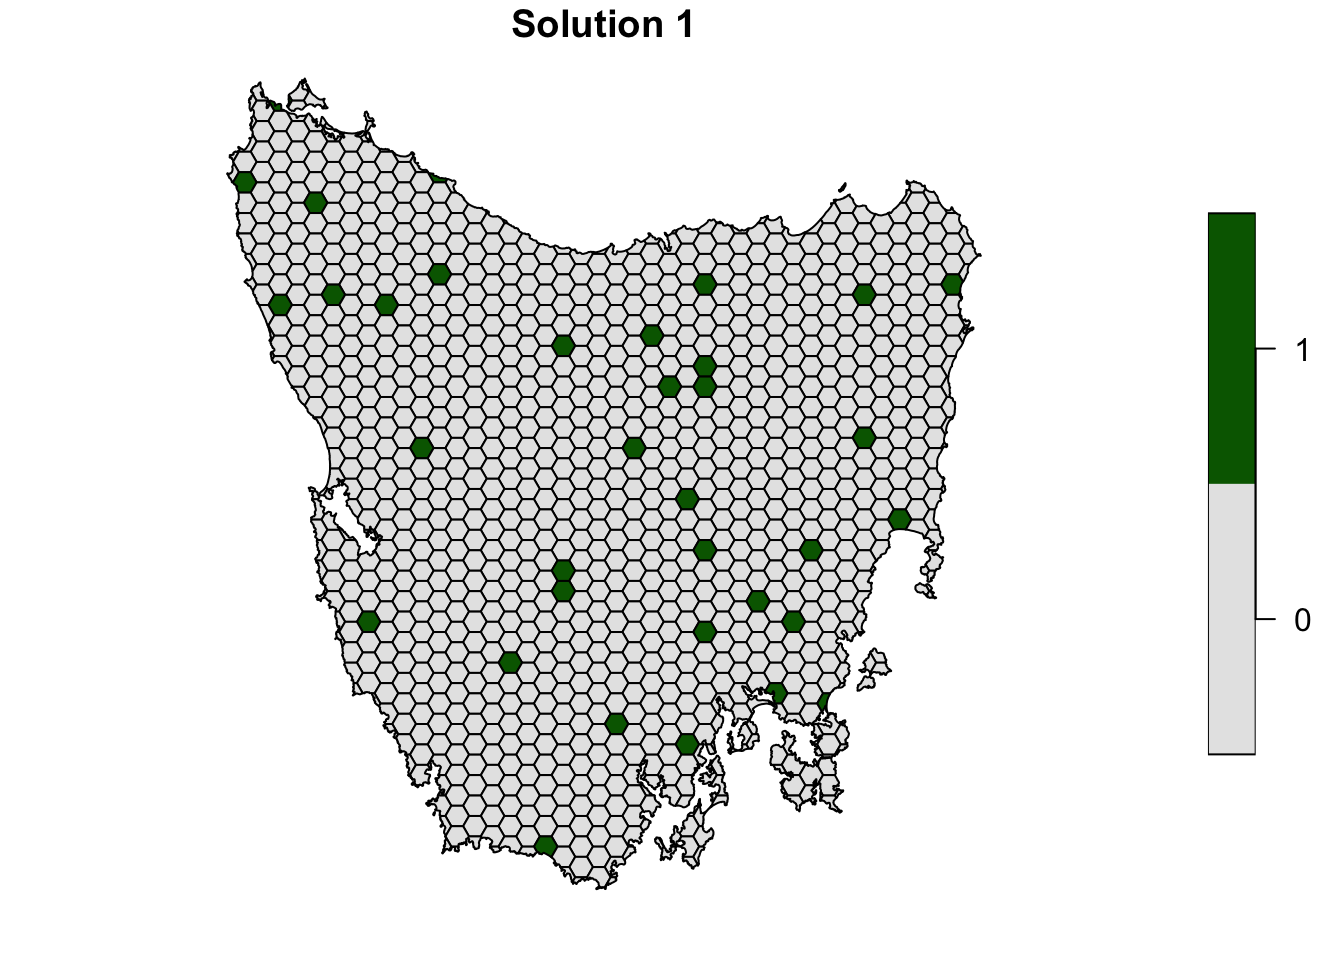
\includegraphics[width=0.65\linewidth]{SpatialPlanning_Workshop2021_files/figure-latex/unnamed-chunk-69-1} \end{center}

Now let's examine the solution.

\begin{rmdquestion}
\begin{enumerate}
\def\labelenumi{\arabic{enumi}.}
\tightlist
\item
  How many planing units were selected in the prioritization? What proportion of planning units were selected in the prioritization?
\item
  Is there a pattern in the spatial distribution of the priority areas?
\item
  Can you verify that all of the targets were met in the prioritization (hint: \texttt{feature\_representation(p1,\ s1{[},\ "solution\_1"{]})})?
\end{enumerate}
\end{rmdquestion}

\hypertarget{adding-complexity}{%
\section{Adding complexity}\label{adding-complexity}}

Our first prioritization suffers many limitations, so let's add additional constraints to the problem to make it more useful.

First, let's lock in planing units that are already by covered protected areas. If some vegetation communities are already secured inside existing protected areas, then we might not need to add as many new protected areas to the existing protected area system to meet their targets. Since our planning unit data (\texttt{tas\_pu}) already contains this information in the \texttt{locked\_in} column, we can use this column name to specify which planning units should be locked in.

\begin{Shaded}
\begin{Highlighting}[]
\CommentTok{\# make prioritization problem}
\NormalTok{p2 }\OtherTok{\textless{}{-}} \FunctionTok{problem}\NormalTok{(tas\_pu, tas\_features, }\AttributeTok{cost\_column =} \StringTok{"cost"}\NormalTok{) }\SpecialCharTok{\%\textgreater{}\%}
      \FunctionTok{add\_min\_set\_objective}\NormalTok{() }\SpecialCharTok{\%\textgreater{}\%}
      \FunctionTok{add\_relative\_targets}\NormalTok{(}\FloatTok{0.05}\NormalTok{) }\SpecialCharTok{\%\textgreater{}\%}
      \FunctionTok{add\_locked\_in\_constraints}\NormalTok{(}\StringTok{"locked\_in"}\NormalTok{) }\SpecialCharTok{\%\textgreater{}\%}
      \FunctionTok{add\_binary\_decisions}\NormalTok{() }\SpecialCharTok{\%\textgreater{}\%}
      \FunctionTok{add\_gurobi\_solver}\NormalTok{(}\AttributeTok{verbose =} \ConstantTok{FALSE}\NormalTok{)}
      \CommentTok{\# add\_lpsymphony\_solver(verbose = FALSE)}

\CommentTok{\# print problem}
\FunctionTok{print}\NormalTok{(p2)}
\end{Highlighting}
\end{Shaded}

\begin{verbatim}
## Conservation Problem
##   planning units: SpatialPolygonsDataFrame (1130 units)
##   cost:           min: 0.19249, max: 61.92727
##   features:       vegetation.1, vegetation.2, vegetation.3, ... (62 features)
##   objective:      Minimum set objective 
##   targets:        Relative targets [targets (min: 0.05, max: 0.05)]
##   decisions:      Binary decision 
##   constraints:    <Locked in planning units [257 locked units]>
##   penalties:      <none>
##   portfolio:      default
##   solver:         Gurobi [first_feasible (0), gap (0.1), numeric_focus (0), presolve (2), threads (1), time_limit (2147483647), verbose (0)]
\end{verbatim}

\begin{Shaded}
\begin{Highlighting}[]
\CommentTok{\# solve problem}
\NormalTok{s2 }\OtherTok{\textless{}{-}} \FunctionTok{solve}\NormalTok{(p2)}

\CommentTok{\# plot solution}
\FunctionTok{plot\_solution}\NormalTok{(s2)}
\end{Highlighting}
\end{Shaded}

\begin{center}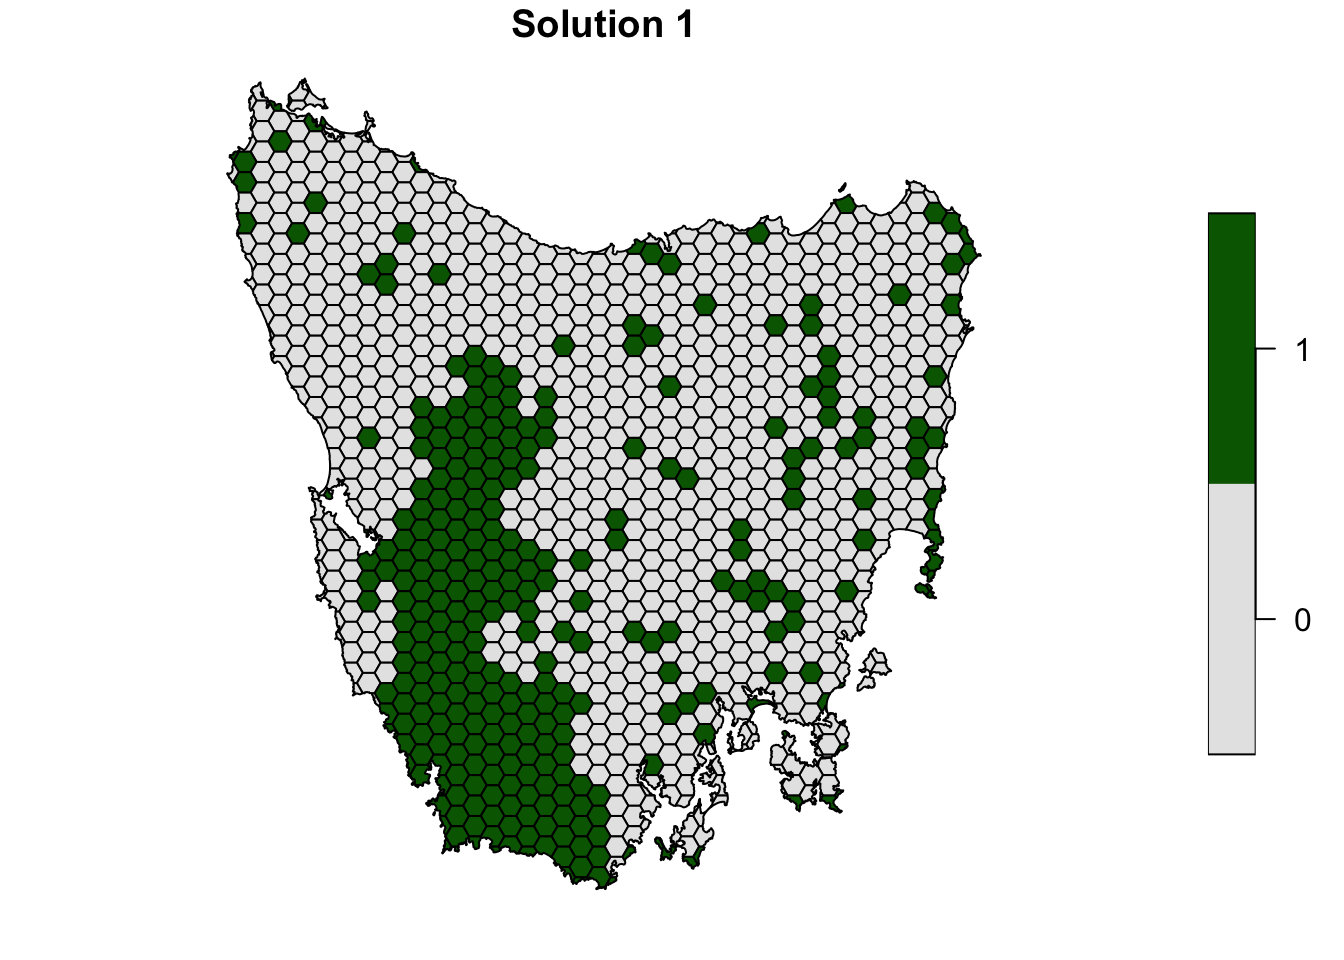
\includegraphics[width=0.65\linewidth]{SpatialPlanning_Workshop2021_files/figure-latex/unnamed-chunk-71-1} \end{center}

Let's pretend that we talked to an expert on the vegetation communities in our study system and they recommended that a 20\% target was needed for each vegetation class. So, armed with this information, let's set the targets to 20\%.

\begin{Shaded}
\begin{Highlighting}[]
\CommentTok{\# make prioritization problem}
\NormalTok{p3 }\OtherTok{\textless{}{-}} \FunctionTok{problem}\NormalTok{(tas\_pu, tas\_features, }\AttributeTok{cost\_column =} \StringTok{"cost"}\NormalTok{) }\SpecialCharTok{\%\textgreater{}\%}
      \FunctionTok{add\_min\_set\_objective}\NormalTok{() }\SpecialCharTok{\%\textgreater{}\%}
      \FunctionTok{add\_relative\_targets}\NormalTok{(}\FloatTok{0.2}\NormalTok{) }\SpecialCharTok{\%\textgreater{}\%}
      \FunctionTok{add\_locked\_in\_constraints}\NormalTok{(}\StringTok{"locked\_in"}\NormalTok{) }\SpecialCharTok{\%\textgreater{}\%}
      \FunctionTok{add\_binary\_decisions}\NormalTok{() }\SpecialCharTok{\%\textgreater{}\%}
      \FunctionTok{add\_gurobi\_solver}\NormalTok{(}\AttributeTok{verbose =} \ConstantTok{FALSE}\NormalTok{)}
      \CommentTok{\# add\_lpsymphony\_solver(verbose = FALSE)}

\CommentTok{\# print problem}
\FunctionTok{print}\NormalTok{(p3)}
\end{Highlighting}
\end{Shaded}

\begin{verbatim}
## Conservation Problem
##   planning units: SpatialPolygonsDataFrame (1130 units)
##   cost:           min: 0.19249, max: 61.92727
##   features:       vegetation.1, vegetation.2, vegetation.3, ... (62 features)
##   objective:      Minimum set objective 
##   targets:        Relative targets [targets (min: 0.2, max: 0.2)]
##   decisions:      Binary decision 
##   constraints:    <Locked in planning units [257 locked units]>
##   penalties:      <none>
##   portfolio:      default
##   solver:         Gurobi [first_feasible (0), gap (0.1), numeric_focus (0), presolve (2), threads (1), time_limit (2147483647), verbose (0)]
\end{verbatim}

\begin{Shaded}
\begin{Highlighting}[]
\CommentTok{\# solve problem}
\NormalTok{s3 }\OtherTok{\textless{}{-}} \FunctionTok{solve}\NormalTok{(p3)}

\CommentTok{\# plot solution}
\FunctionTok{plot\_solution}\NormalTok{(s3)}
\end{Highlighting}
\end{Shaded}

\begin{center}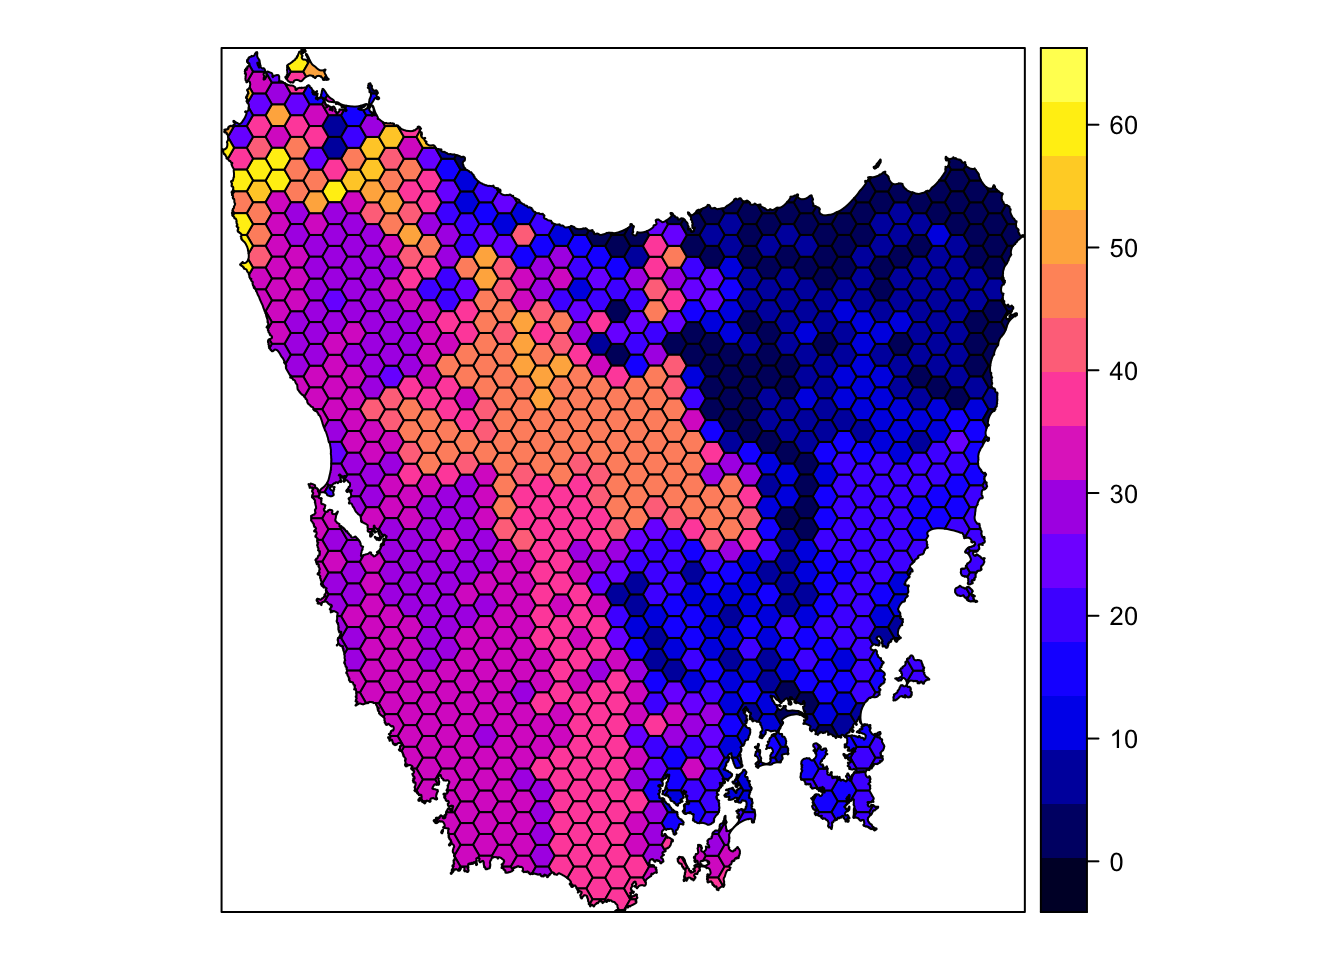
\includegraphics[width=0.65\linewidth]{SpatialPlanning_Workshop2021_files/figure-latex/unnamed-chunk-72-1} \end{center}

Next, let's lock out highly degraded areas. Similar to before, this data is present in our planning unit data so we can use the \texttt{locked\_out} column name to achieve this.

\begin{Shaded}
\begin{Highlighting}[]
\CommentTok{\# make prioritization problem}
\NormalTok{p4 }\OtherTok{\textless{}{-}} \FunctionTok{problem}\NormalTok{(tas\_pu, tas\_features, }\AttributeTok{cost\_column =} \StringTok{"cost"}\NormalTok{) }\SpecialCharTok{\%\textgreater{}\%}
      \FunctionTok{add\_min\_set\_objective}\NormalTok{() }\SpecialCharTok{\%\textgreater{}\%}
      \FunctionTok{add\_relative\_targets}\NormalTok{(}\FloatTok{0.2}\NormalTok{) }\SpecialCharTok{\%\textgreater{}\%}
      \FunctionTok{add\_locked\_in\_constraints}\NormalTok{(}\StringTok{"locked\_in"}\NormalTok{) }\SpecialCharTok{\%\textgreater{}\%}
      \FunctionTok{add\_locked\_out\_constraints}\NormalTok{(}\StringTok{"locked\_out"}\NormalTok{) }\SpecialCharTok{\%\textgreater{}\%}
      \FunctionTok{add\_binary\_decisions}\NormalTok{() }\SpecialCharTok{\%\textgreater{}\%}
      \FunctionTok{add\_gurobi\_solver}\NormalTok{(}\AttributeTok{verbose =} \ConstantTok{FALSE}\NormalTok{)}
      \CommentTok{\# add\_lpsymphony\_solver(verbose = FALSE)}
\end{Highlighting}
\end{Shaded}

\begin{Shaded}
\begin{Highlighting}[]
\CommentTok{\# print problem}
\FunctionTok{print}\NormalTok{(p4)}
\end{Highlighting}
\end{Shaded}

\begin{verbatim}
## Conservation Problem
##   planning units: SpatialPolygonsDataFrame (1130 units)
##   cost:           min: 0.19249, max: 61.92727
##   features:       vegetation.1, vegetation.2, vegetation.3, ... (62 features)
##   objective:      Minimum set objective 
##   targets:        Relative targets [targets (min: 0.2, max: 0.2)]
##   decisions:      Binary decision 
##   constraints:    <Locked out planning units [45 locked units]
##                    Locked in planning units [257 locked units]>
##   penalties:      <none>
##   portfolio:      default
##   solver:         Gurobi [first_feasible (0), gap (0.1), numeric_focus (0), presolve (2), threads (1), time_limit (2147483647), verbose (0)]
\end{verbatim}

\begin{Shaded}
\begin{Highlighting}[]
\CommentTok{\# solve problem}
\NormalTok{s4 }\OtherTok{\textless{}{-}} \FunctionTok{solve}\NormalTok{(p4)}

\CommentTok{\# plot solution}
\FunctionTok{spplot}\NormalTok{(s4, }\StringTok{"solution\_1"}\NormalTok{, }\AttributeTok{col.regions =} \FunctionTok{c}\NormalTok{(}\StringTok{"white"}\NormalTok{, }\StringTok{"darkgreen"}\NormalTok{), }\AttributeTok{main =} \StringTok{"s4"}\NormalTok{)}
\end{Highlighting}
\end{Shaded}

\begin{center}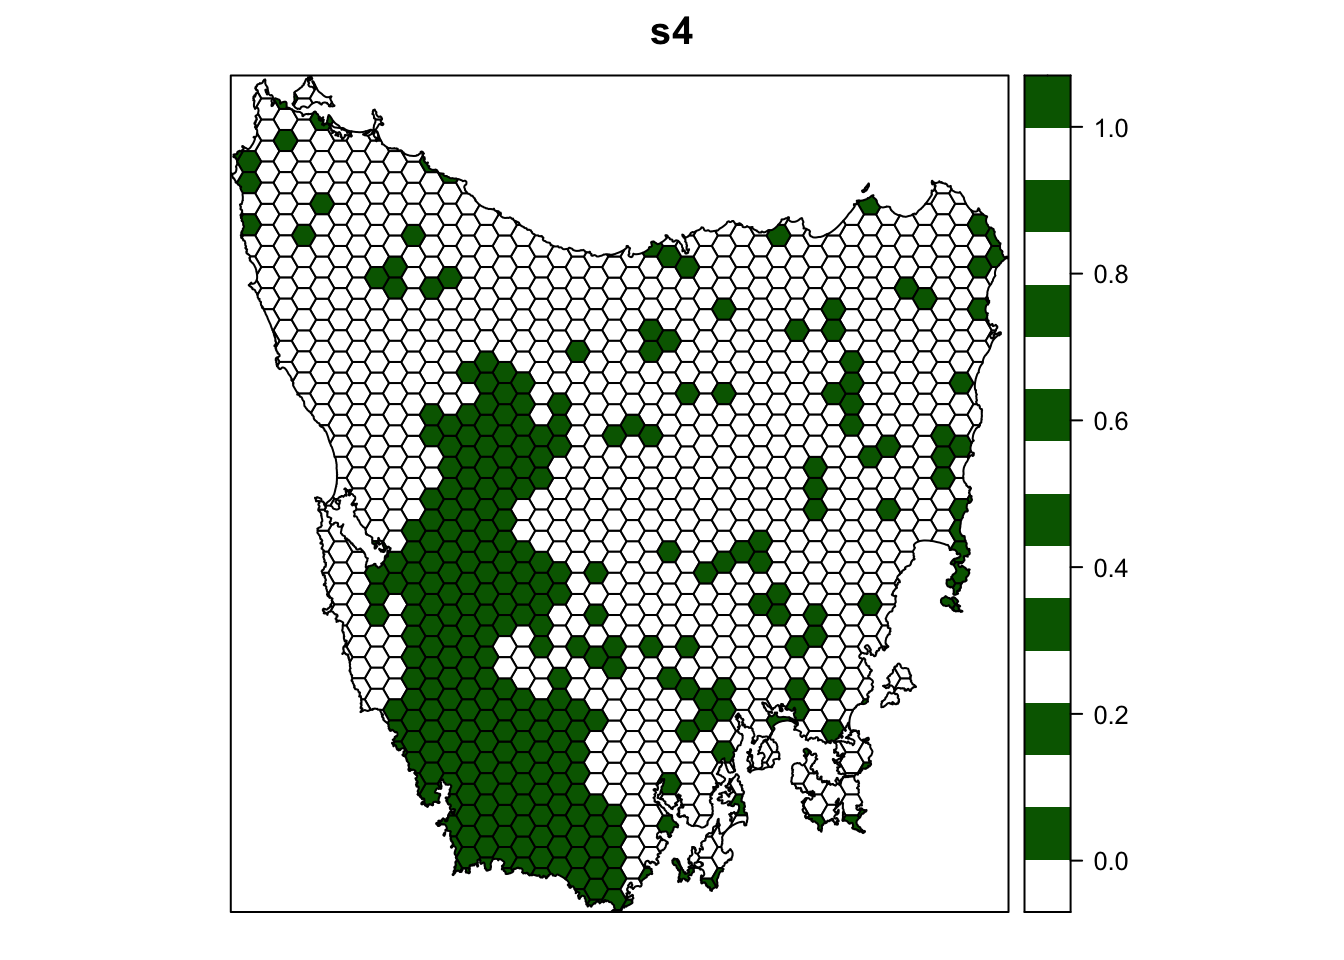
\includegraphics[width=0.65\linewidth]{SpatialPlanning_Workshop2021_files/figure-latex/unnamed-chunk-74-1} \end{center}

\begin{Shaded}
\begin{Highlighting}[]
\FunctionTok{plot\_solution}\NormalTok{(s4)}
\end{Highlighting}
\end{Shaded}

\begin{center}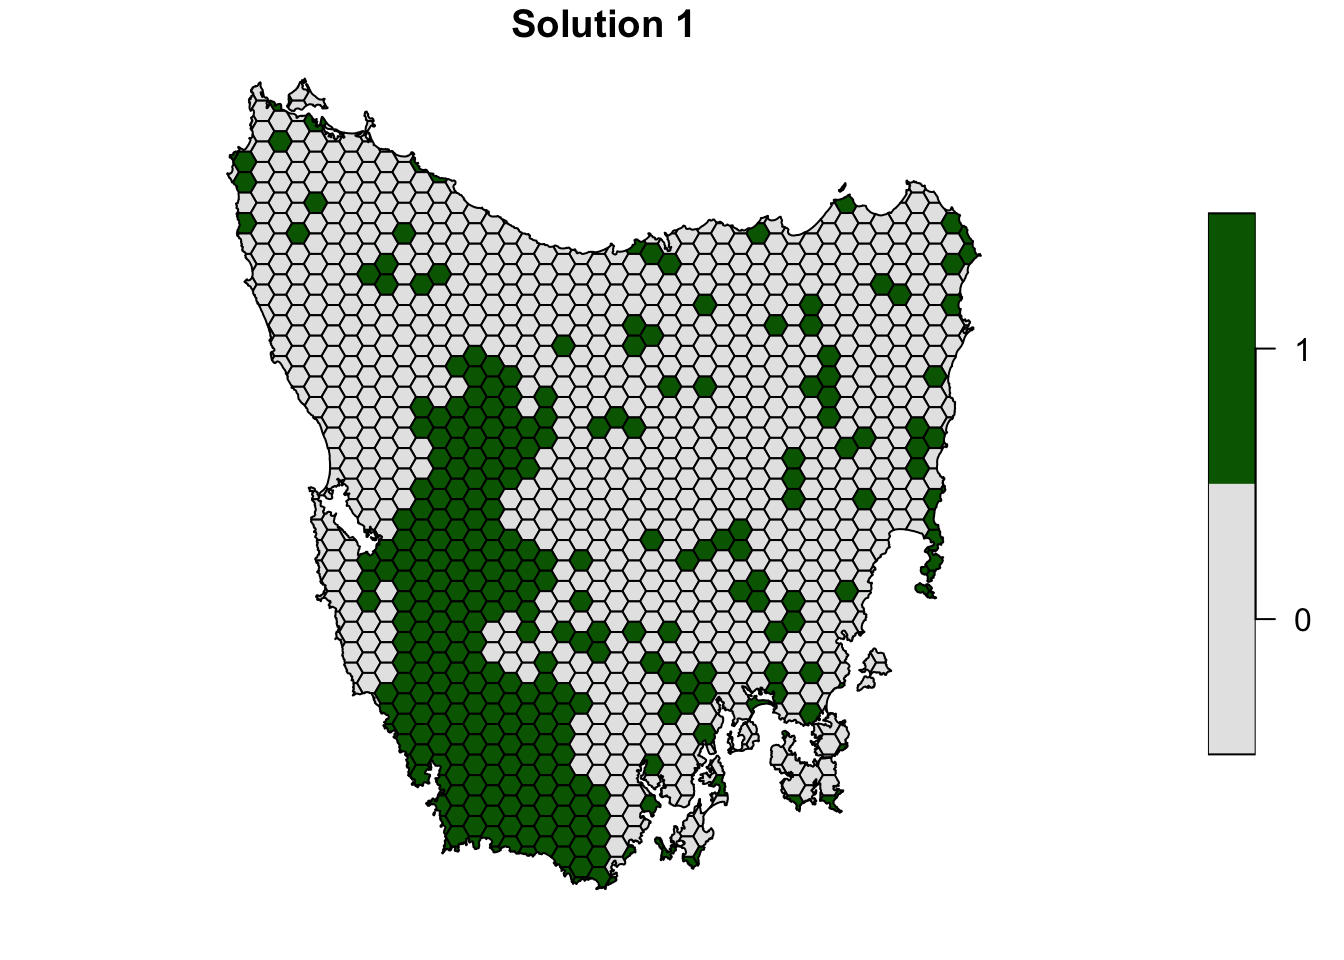
\includegraphics[width=0.65\linewidth]{SpatialPlanning_Workshop2021_files/figure-latex/unnamed-chunk-74-2} \end{center}

\clearpage

Now, let's compare the solutions.

\begin{rmdquestion}
\begin{enumerate}
\def\labelenumi{\arabic{enumi}.}
\tightlist
\item
  What is the cost of the planning units selected in \texttt{s2}, \texttt{s3}, and \texttt{s4}?
\item
  How many planning units are in \texttt{s2}, \texttt{s3}, and \texttt{s4}?
\item
  Do the solutions with more planning units have a greater cost? Why or why not?
\item
  Why does the first solution (\texttt{s1}) cost less than the second solution with protected areas locked into the solution (\texttt{s2})?
\item
  Why does the third solution (\texttt{s3}) cost less than the fourth solution solution with highly degraded areas locked out (\texttt{s4})?
\item
  Since planning units covered by existing protected areas have already been purchased, what is the cost for expanding the protected area system based on on the fourth prioritization (\texttt{s4}) (hint: total cost minus the cost of locked in planning units)?
\item
  What happens if you specify targets that exceed the total amount of vegetation in the study area and try to solve the problem? You can do this by modifying the code to make \texttt{p4} with \texttt{add\_absolute\_targets(1000)} instead of \texttt{add\_relative\_targets(0.2)} and generating a new solution.
\end{enumerate}
\end{rmdquestion}

\hypertarget{penalizing-fragmentation}{%
\section{Penalizing fragmentation}\label{penalizing-fragmentation}}

Plans for protected area systems should facilitate gene flow and dispersal between individual reserves in the system. However, the prioritizations we have made so far have been highly fragmented.

We can add penalties to our conservation planning problem to penalize fragmentation (i.e.~total exposed boundary length) and we also need to set a useful penalty value when adding such penalties. If we set our penalty value too low, then we will end up with a solution that is identical to the solution with no added penalties. If we set our penalty value too high, then prioritizr will take a long time to solve the problem and we will end up with a solution that contains lots of extra planning units that are not needed (since the penalty value is so high that minimizing fragmentation is more important than cost). As a rule of thumb, we generally want penalty values between 0.00001 and 0.01 but finding a useful penalty value requires calibration. The ``correct'' penalty value depends on the size of the planning units, the main objective values (e.g.~cost values), and the effect of fragmentation on biodiversity persistence.

Let's create a new problem that is similar to our previous problem (\texttt{p4})---except that it contains boundary length penalties and a slightly higher optimality gap to reduce runtime (default is 0.1)---and solve it. Since our planning unit data is in a spatial format (i.e.~vector or raster data), prioritizr can automatically calculate the boundary data for us.

\clearpage

\begin{Shaded}
\begin{Highlighting}[]
\CommentTok{\# make prioritization problem}
\NormalTok{p5 }\OtherTok{\textless{}{-}} \FunctionTok{problem}\NormalTok{(tas\_pu, tas\_features, }\AttributeTok{cost\_column =} \StringTok{"cost"}\NormalTok{) }\SpecialCharTok{\%\textgreater{}\%}
      \FunctionTok{add\_min\_set\_objective}\NormalTok{() }\SpecialCharTok{\%\textgreater{}\%}
      \FunctionTok{add\_boundary\_penalties}\NormalTok{(}\AttributeTok{penalty =} \FloatTok{0.0005}\NormalTok{) }\SpecialCharTok{\%\textgreater{}\%}
      \FunctionTok{add\_relative\_targets}\NormalTok{(}\FloatTok{0.2}\NormalTok{) }\SpecialCharTok{\%\textgreater{}\%}
      \FunctionTok{add\_locked\_in\_constraints}\NormalTok{(}\StringTok{"locked\_in"}\NormalTok{) }\SpecialCharTok{\%\textgreater{}\%}
      \FunctionTok{add\_locked\_out\_constraints}\NormalTok{(}\StringTok{"locked\_out"}\NormalTok{) }\SpecialCharTok{\%\textgreater{}\%}
      \FunctionTok{add\_binary\_decisions}\NormalTok{() }\SpecialCharTok{\%\textgreater{}\%}
      \FunctionTok{add\_gurobi\_solver}\NormalTok{(}\AttributeTok{verbose =} \ConstantTok{FALSE}\NormalTok{)}
      \CommentTok{\# add\_lpsymphony\_solver(verbose = FALSE)}

\CommentTok{\# print problem}
\FunctionTok{print}\NormalTok{(p5)}
\end{Highlighting}
\end{Shaded}

\begin{verbatim}
## Conservation Problem
##   planning units: SpatialPolygonsDataFrame (1130 units)
##   cost:           min: 0.19249, max: 61.92727
##   features:       vegetation.1, vegetation.2, vegetation.3, ... (62 features)
##   objective:      Minimum set objective 
##   targets:        Relative targets [targets (min: 0.2, max: 0.2)]
##   decisions:      Binary decision 
##   constraints:    <Locked out planning units [45 locked units]
##                    Locked in planning units [257 locked units]>
##   penalties:      <Boundary penalties [edge factor (min: 0.5, max: 0.5), penalty (5e-04), zones]>
##   portfolio:      default
##   solver:         Gurobi [first_feasible (0), gap (0.1), numeric_focus (0), presolve (2), threads (1), time_limit (2147483647), verbose (0)]
\end{verbatim}

\begin{Shaded}
\begin{Highlighting}[]
\CommentTok{\# solve problem,}
\CommentTok{\# note this will take around 30 seconds}
\NormalTok{s5 }\OtherTok{\textless{}{-}} \FunctionTok{solve}\NormalTok{(p5)}

\CommentTok{\# print solution}
\FunctionTok{print}\NormalTok{(s5)}
\end{Highlighting}
\end{Shaded}

\begin{verbatim}
## class       : SpatialPolygonsDataFrame 
## features    : 1130 
## extent      : 1080623, 1399989, -4840595, -4497092  (xmin, xmax, ymin, ymax)
## crs         : +proj=aea +lat_0=0 +lon_0=132 +lat_1=-18 +lat_2=-36 +x_0=0 +y_0=0 +ellps=GRS80 +units=m +no_defs 
## variables   : 6
## names       :   id,              cost, status, locked_in, locked_out, solution_1 
## min values  :    1, 0.192488262910798,      0,         0,          0,          0 
## max values  : 1130,  61.9272727272727,      2,         1,          1,          1
\end{verbatim}

\begin{Shaded}
\begin{Highlighting}[]
\CommentTok{\# plot solution}
\FunctionTok{plot\_solution}\NormalTok{(s5)}
\end{Highlighting}
\end{Shaded}

\begin{center}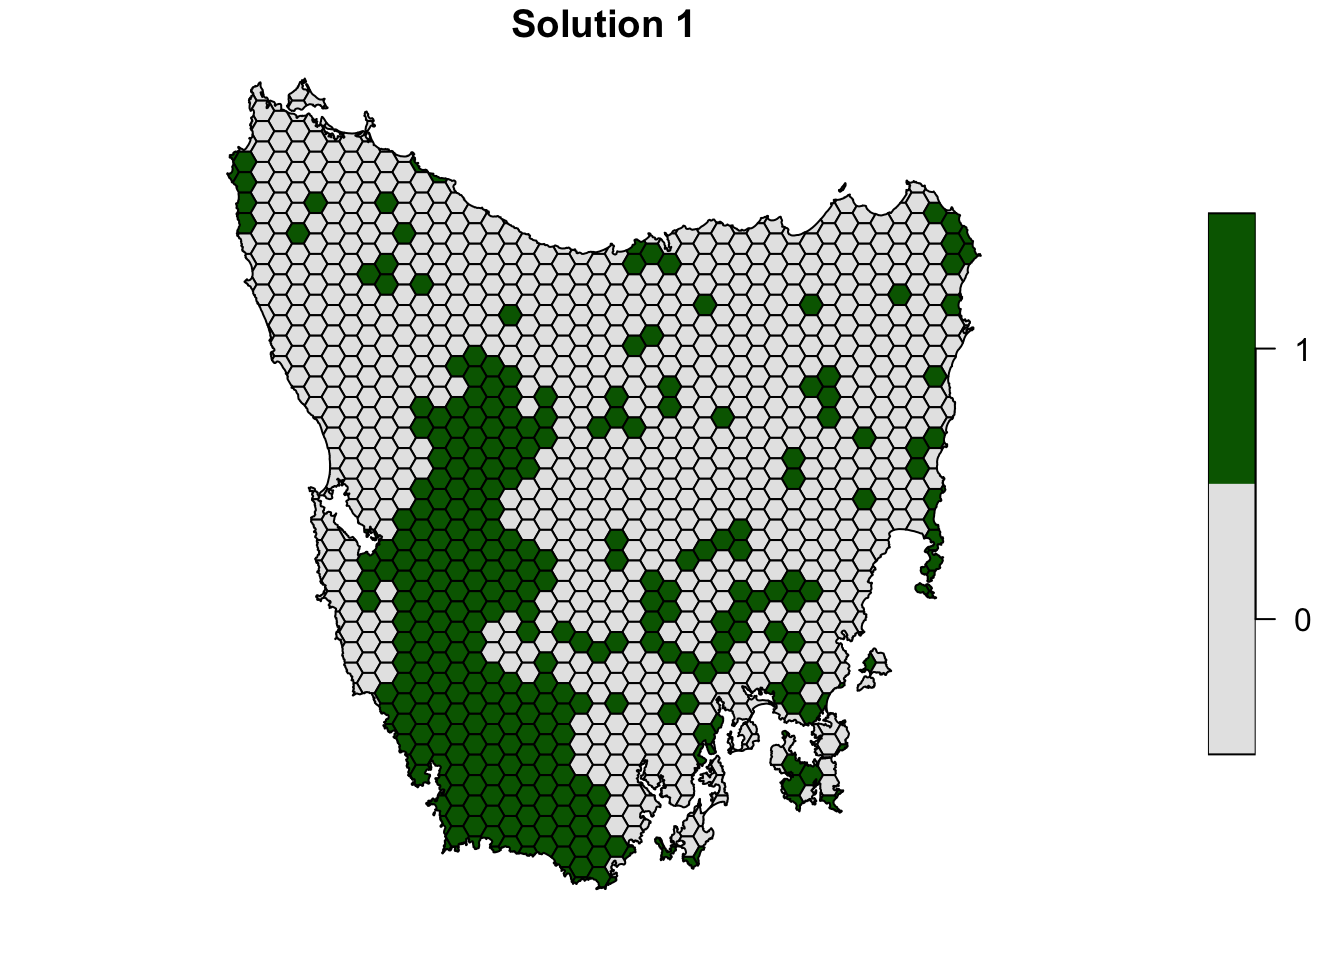
\includegraphics[width=0.65\linewidth]{SpatialPlanning_Workshop2021_files/figure-latex/unnamed-chunk-76-1} \end{center}

Now let's compare the solutions to the problems with (\texttt{s5}) and without (\texttt{s4}) the boundary length penalties.

\begin{rmdquestion}
\begin{enumerate}
\def\labelenumi{\arabic{enumi}.}
\tightlist
\item
  What is the cost the fourth (\texttt{s4}) and fifth (\texttt{s5}) solutions? Why does the fifth solution (\texttt{s5}) cost more than the fourth (\texttt{s4}) solution?
\item
  Try setting the penalty value to 0.000000001 (i.e.~\texttt{1e-9}) instead of 0.0005. What is the cost of the solution now? Is it different from the fourth solution (\texttt{s4}) (hint: try plotting the solutions to visualize them)? Is this is a useful penalty value? Why?
\item
  Try setting the penalty value to 0.5. What is the cost of the solution now? Is it different from the fourth solution (\texttt{s4}) (hint: try plotting the solutions to visualize them)? Is this a useful penalty value? Why?
\end{enumerate}
\end{rmdquestion}

\clearpage

\hypertarget{budget-limited-prioritizations}{%
\section{Budget limited prioritizations}\label{budget-limited-prioritizations}}

In the real-world, the funding available for conservation is often very limited. As a consequence, decision makers often need prioritizations where the total cost of priority areas does not exceed a budget.

In our fourth prioritization (\texttt{s4}), we found that we would need to spend an additional \$1317 million AUD to ensure that each vegetation community is adequately represented in the protected area system. But what if the funds available for establishing new protected areas were limited to \$100 million AUD? In this case, we need a ``budget limited prioritization''. Budget limited prioritizations aim to maximize some measure of conservation benefit subject to a budget (e.g.~\href{https://prioritizr.net/reference/add_max_cover_objective.html}{number of species with at least one occurrence in the protected area system}, or \href{https://prioritizr.net/reference/add_max_phylo_div_objective.html}{phylogenetic diversity}). Let's create a prioritization by maximizing the number of adequately represented features whilst keeping within a pre-specified budget.

\begin{Shaded}
\begin{Highlighting}[]
\CommentTok{\# funds for additional land acquisition (same units as cost data)}
\NormalTok{funds }\OtherTok{\textless{}{-}} \DecValTok{100}

\CommentTok{\# calculate the total budget for the prioritization}
\NormalTok{budget }\OtherTok{\textless{}{-}}\NormalTok{ funds }\SpecialCharTok{+} \FunctionTok{sum}\NormalTok{(s4}\SpecialCharTok{$}\NormalTok{cost }\SpecialCharTok{*}\NormalTok{ s4}\SpecialCharTok{$}\NormalTok{locked\_in)}
\FunctionTok{print}\NormalTok{(budget)}
\end{Highlighting}
\end{Shaded}

\begin{verbatim}
## [1] 8575.56
\end{verbatim}

\begin{Shaded}
\begin{Highlighting}[]
\CommentTok{\# make prioritization problem}
\NormalTok{p6 }\OtherTok{\textless{}{-}} \FunctionTok{problem}\NormalTok{(tas\_pu, tas\_features, }\AttributeTok{cost\_column =} \StringTok{"cost"}\NormalTok{) }\SpecialCharTok{\%\textgreater{}\%}
      \FunctionTok{add\_max\_features\_objective}\NormalTok{(budget) }\SpecialCharTok{\%\textgreater{}\%}
      \FunctionTok{add\_relative\_targets}\NormalTok{(}\FloatTok{0.2}\NormalTok{) }\SpecialCharTok{\%\textgreater{}\%}
      \FunctionTok{add\_locked\_in\_constraints}\NormalTok{(}\StringTok{"locked\_in"}\NormalTok{) }\SpecialCharTok{\%\textgreater{}\%}
      \FunctionTok{add\_locked\_out\_constraints}\NormalTok{(}\StringTok{"locked\_out"}\NormalTok{) }\SpecialCharTok{\%\textgreater{}\%}
      \FunctionTok{add\_binary\_decisions}\NormalTok{() }\SpecialCharTok{\%\textgreater{}\%}
      \FunctionTok{add\_gurobi\_solver}\NormalTok{(}\AttributeTok{verbose =} \ConstantTok{FALSE}\NormalTok{)}
      \CommentTok{\# add\_lpsymphony\_solver(verbose = FALSE)}

\CommentTok{\# print problem}
\FunctionTok{print}\NormalTok{(p6)}
\end{Highlighting}
\end{Shaded}

\begin{verbatim}
## Conservation Problem
##   planning units: SpatialPolygonsDataFrame (1130 units)
##   cost:           min: 0.19249, max: 61.92727
##   features:       vegetation.1, vegetation.2, vegetation.3, ... (62 features)
##   objective:      Maximum representation objective [budget (8575.56009869836)]
##   targets:        Relative targets [targets (min: 0.2, max: 0.2)]
##   decisions:      Binary decision 
##   constraints:    <Locked in planning units [257 locked units]
##                    Locked out planning units [45 locked units]>
##   penalties:      <none>
##   portfolio:      default
##   solver:         Gurobi [first_feasible (0), gap (0.1), numeric_focus (0), presolve (2), threads (1), time_limit (2147483647), verbose (0)]
\end{verbatim}

\begin{Shaded}
\begin{Highlighting}[]
\CommentTok{\# solve problem}
\NormalTok{s6 }\OtherTok{\textless{}{-}} \FunctionTok{solve}\NormalTok{(p6)}

\CommentTok{\# plot solution}
\FunctionTok{plot\_solution}\NormalTok{(s6)}
\end{Highlighting}
\end{Shaded}

\begin{center}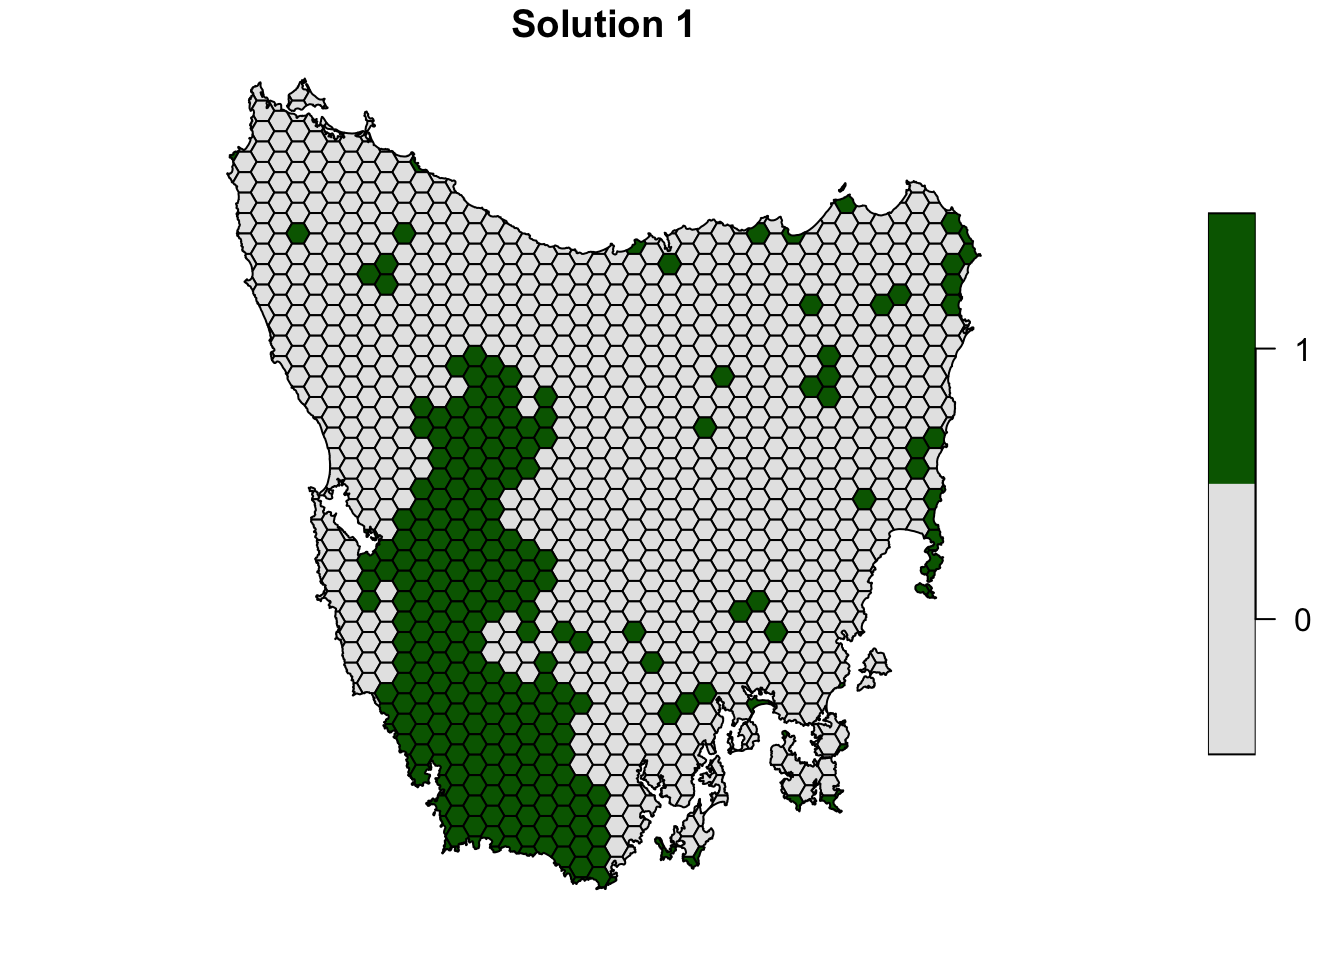
\includegraphics[width=0.65\linewidth]{SpatialPlanning_Workshop2021_files/figure-latex/budget-1} \end{center}

\begin{Shaded}
\begin{Highlighting}[]
\CommentTok{\# calculate feature representation}
\NormalTok{r6 }\OtherTok{\textless{}{-}} \FunctionTok{eval\_feature\_representation\_summary}\NormalTok{(p6, s6[, }\StringTok{"solution\_1"}\NormalTok{])}

\CommentTok{\# calculate number of features with targets met}
\FunctionTok{sum}\NormalTok{(r6}\SpecialCharTok{$}\NormalTok{relative\_held }\SpecialCharTok{\textgreater{}=} \FloatTok{0.2}\NormalTok{, }\AttributeTok{na.rm =} \ConstantTok{TRUE}\NormalTok{)}
\end{Highlighting}
\end{Shaded}

\begin{verbatim}
## [1] 28
\end{verbatim}

\begin{Shaded}
\begin{Highlighting}[]
\CommentTok{\# find out which features have their targets met when we add weights,}
\CommentTok{\# note that NA is for vegetation.61}
\FunctionTok{print}\NormalTok{(r6}\SpecialCharTok{$}\NormalTok{feature[r6}\SpecialCharTok{$}\NormalTok{relative\_held }\SpecialCharTok{\textgreater{}=} \FloatTok{0.2}\NormalTok{])}
\end{Highlighting}
\end{Shaded}

\begin{verbatim}
##  [1] "vegetation.1"  "vegetation.2"  "vegetation.3"  "vegetation.4" 
##  [5] "vegetation.5"  "vegetation.6"  "vegetation.7"  "vegetation.8" 
##  [9] "vegetation.11" "vegetation.12" "vegetation.15" "vegetation.17"
## [13] "vegetation.22" "vegetation.23" "vegetation.25" "vegetation.28"
## [17] "vegetation.29" "vegetation.30" "vegetation.32" "vegetation.33"
## [21] "vegetation.34" "vegetation.35" "vegetation.36" "vegetation.37"
## [25] "vegetation.38" "vegetation.39" "vegetation.40" "vegetation.45"
\end{verbatim}

We can also add weights to specify that it is more important to meet the targets for certain features and less important for other features. A common approach for weighting features is to assign a greater importance to features with smaller spatial distributions. The rationale behind this weighting method is that features with smaller spatial distributions are at greater risk of extinction.

So, let's calculate some weights for our vegetation communities and see how weighting the features changes our prioritization.

\begin{Shaded}
\begin{Highlighting}[]
\CommentTok{\# calculate weights as the log inverse number of grid cells that each vegetation}
\CommentTok{\# class occupies, rescaled between 1 and 100}
\NormalTok{wts }\OtherTok{\textless{}{-}} \DecValTok{1} \SpecialCharTok{/} \FunctionTok{cellStats}\NormalTok{(tas\_features, }\StringTok{"sum"}\NormalTok{)}
\NormalTok{wts }\OtherTok{\textless{}{-}} \FunctionTok{rescale}\NormalTok{(wts, }\AttributeTok{to =} \FunctionTok{c}\NormalTok{(}\DecValTok{1}\NormalTok{, }\DecValTok{10}\NormalTok{))}

\CommentTok{\# print the name of the feature with smallest weight}
\FunctionTok{names}\NormalTok{(tas\_features)[}\FunctionTok{which.min}\NormalTok{(wts)]}
\end{Highlighting}
\end{Shaded}

\begin{verbatim}
## [1] "vegetation.20"
\end{verbatim}

\begin{Shaded}
\begin{Highlighting}[]
\CommentTok{\# print the name of the feature with greatest weight}
\FunctionTok{names}\NormalTok{(tas\_features)[}\FunctionTok{which.max}\NormalTok{(wts)]}
\end{Highlighting}
\end{Shaded}

\begin{verbatim}
## [1] "vegetation.52"
\end{verbatim}

\begin{Shaded}
\begin{Highlighting}[]
\CommentTok{\# plot histogram of weights}
\FunctionTok{hist}\NormalTok{(wts, }\AttributeTok{main =} \StringTok{"feature weights"}\NormalTok{)}
\end{Highlighting}
\end{Shaded}

\begin{center}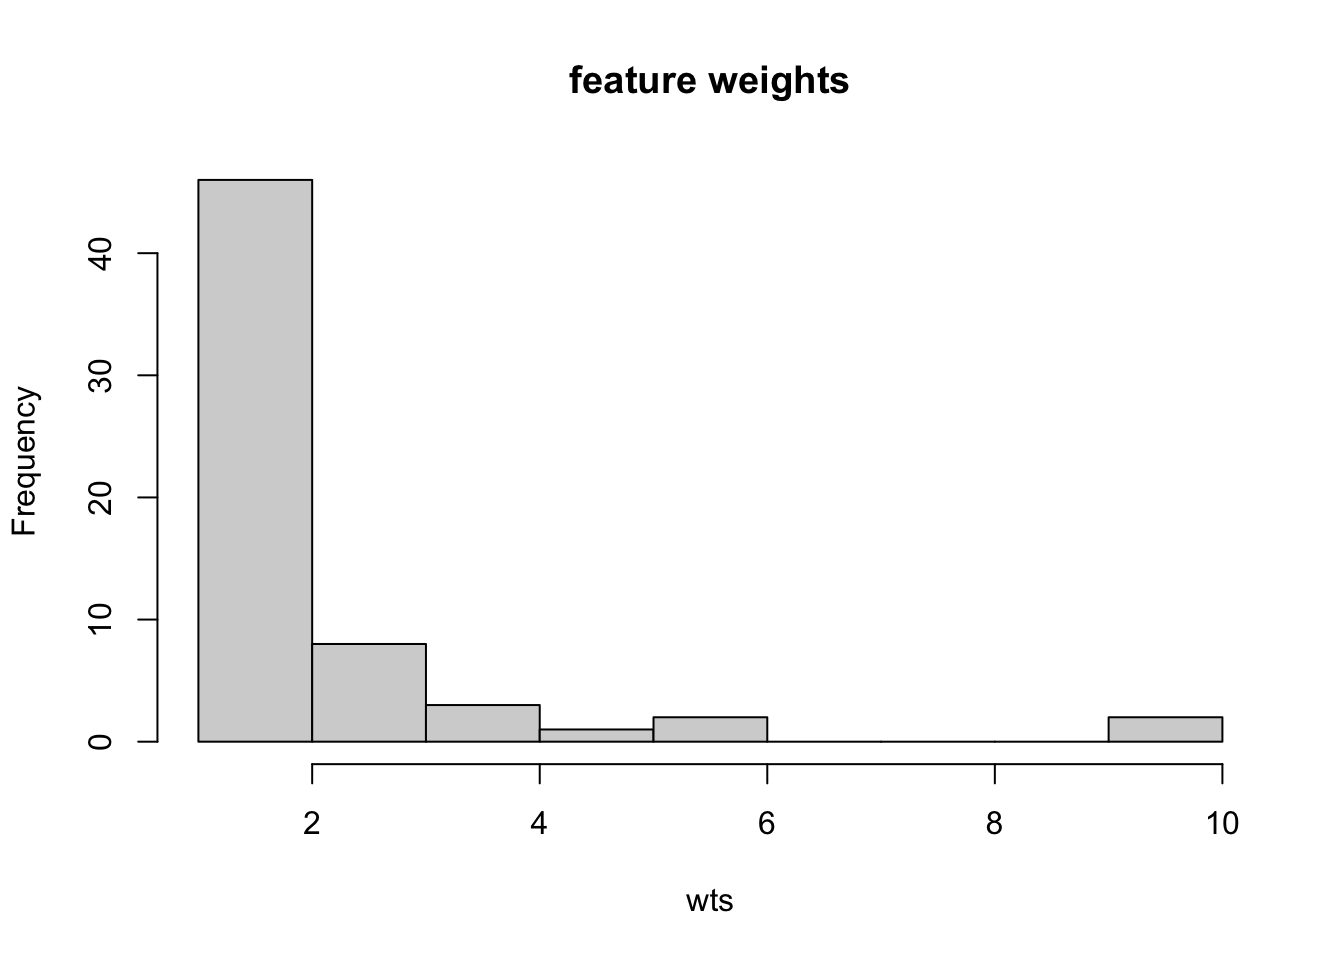
\includegraphics[width=0.65\linewidth]{SpatialPlanning_Workshop2021_files/figure-latex/budget-weights-1} \end{center}

\begin{Shaded}
\begin{Highlighting}[]
\CommentTok{\# make prioritization problem with weights}
\NormalTok{p7 }\OtherTok{\textless{}{-}} \FunctionTok{problem}\NormalTok{(tas\_pu, tas\_features, }\AttributeTok{cost\_column =} \StringTok{"cost"}\NormalTok{) }\SpecialCharTok{\%\textgreater{}\%}
      \FunctionTok{add\_max\_features\_objective}\NormalTok{(budget) }\SpecialCharTok{\%\textgreater{}\%}
      \FunctionTok{add\_relative\_targets}\NormalTok{(}\FloatTok{0.2}\NormalTok{) }\SpecialCharTok{\%\textgreater{}\%}
      \FunctionTok{add\_feature\_weights}\NormalTok{(wts) }\SpecialCharTok{\%\textgreater{}\%}
      \FunctionTok{add\_locked\_in\_constraints}\NormalTok{(}\StringTok{"locked\_in"}\NormalTok{) }\SpecialCharTok{\%\textgreater{}\%}
      \FunctionTok{add\_locked\_out\_constraints}\NormalTok{(}\StringTok{"locked\_out"}\NormalTok{) }\SpecialCharTok{\%\textgreater{}\%}
      \FunctionTok{add\_binary\_decisions}\NormalTok{() }\SpecialCharTok{\%\textgreater{}\%}
       \FunctionTok{add\_gurobi\_solver}\NormalTok{(}\AttributeTok{verbose =} \ConstantTok{FALSE}\NormalTok{)}
      \CommentTok{\# add\_lpsymphony\_solver(verbose = FALSE)}

\CommentTok{\# print problem}
\FunctionTok{print}\NormalTok{(p7)}
\end{Highlighting}
\end{Shaded}

\begin{verbatim}
## Conservation Problem
##   planning units: SpatialPolygonsDataFrame (1130 units)
##   cost:           min: 0.19249, max: 61.92727
##   features:       vegetation.1, vegetation.2, vegetation.3, ... (62 features)
##   objective:      Maximum representation objective [budget (8575.56009869836)]
##   targets:        Relative targets [targets (min: 0.2, max: 0.2)]
##   decisions:      Binary decision 
##   constraints:    <Locked out planning units [45 locked units]
##                    Locked in planning units [257 locked units]>
##   penalties:      <Feature weights [weights (min: 1, max: 10)]>
##   portfolio:      default
##   solver:         Gurobi [first_feasible (0), gap (0.1), numeric_focus (0), presolve (2), threads (1), time_limit (2147483647), verbose (0)]
\end{verbatim}

\begin{Shaded}
\begin{Highlighting}[]
\CommentTok{\# solve problem}
\NormalTok{s7 }\OtherTok{\textless{}{-}} \FunctionTok{solve}\NormalTok{(p7)}

\CommentTok{\# plot solution}
\FunctionTok{plot\_solution}\NormalTok{(s7)}
\end{Highlighting}
\end{Shaded}

\begin{center}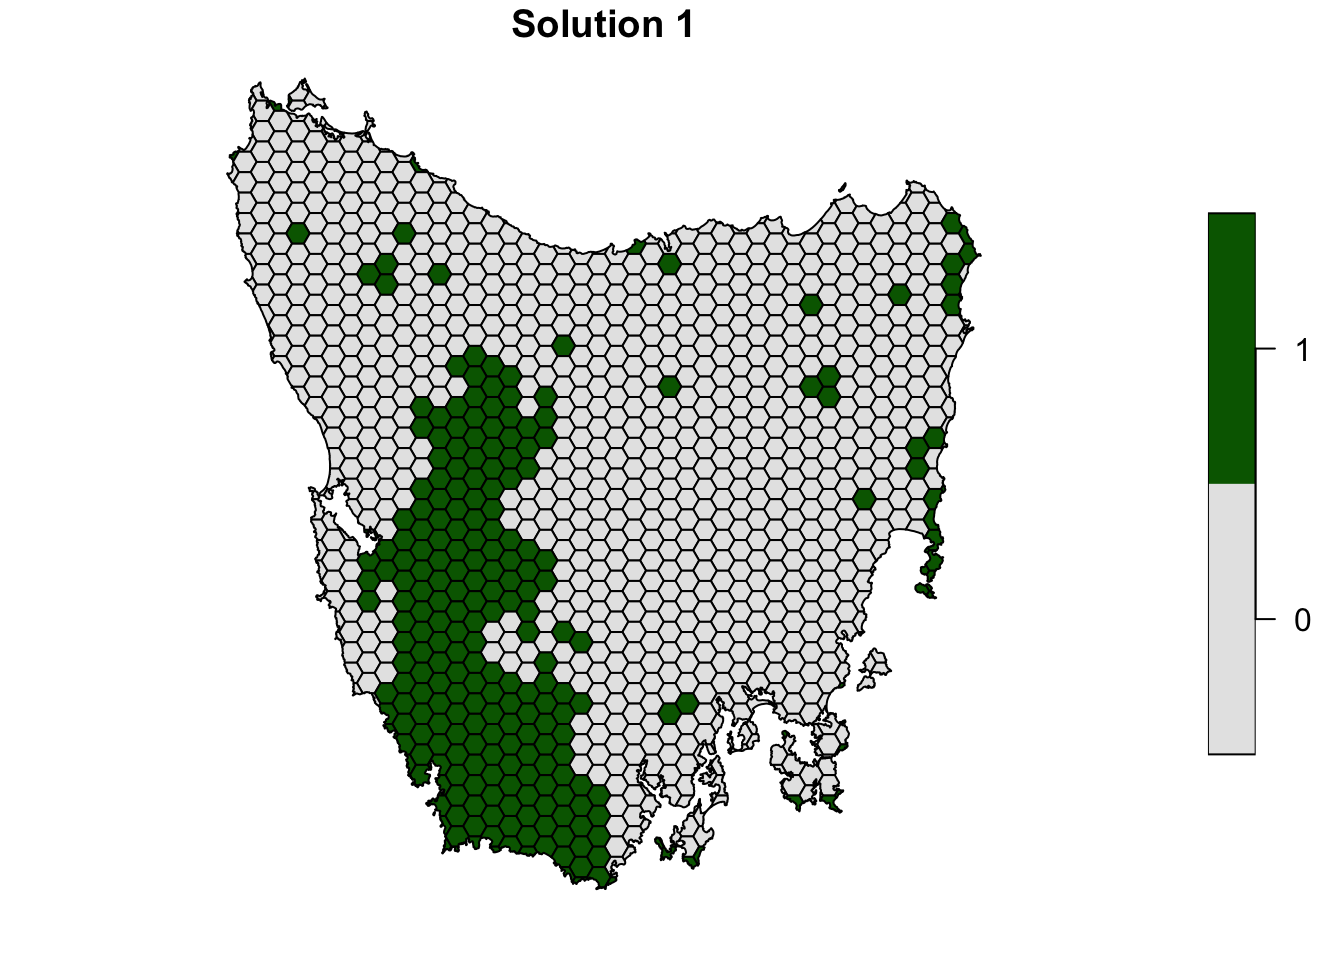
\includegraphics[width=0.65\linewidth]{SpatialPlanning_Workshop2021_files/figure-latex/budget-weights-2} \end{center}

\begin{Shaded}
\begin{Highlighting}[]
\CommentTok{\# calculate feature representation}
\NormalTok{r7 }\OtherTok{\textless{}{-}} \FunctionTok{eval\_feature\_representation\_summary}\NormalTok{(p7, s7[, }\StringTok{"solution\_1"}\NormalTok{])}

\CommentTok{\# calculate number of features with targets met}
\FunctionTok{sum}\NormalTok{(r7}\SpecialCharTok{$}\NormalTok{relative\_held }\SpecialCharTok{\textgreater{}=} \FloatTok{0.2}\NormalTok{, }\AttributeTok{na.rm =} \ConstantTok{TRUE}\NormalTok{)}
\end{Highlighting}
\end{Shaded}

\begin{verbatim}
## [1] 22
\end{verbatim}

\begin{Shaded}
\begin{Highlighting}[]
\CommentTok{\# find out which features have their targets met when we add weights,}
\CommentTok{\# note that NA is for vegetation.61}
\FunctionTok{print}\NormalTok{(r7}\SpecialCharTok{$}\NormalTok{feature[r7}\SpecialCharTok{$}\NormalTok{relative\_held }\SpecialCharTok{\textgreater{}=} \FloatTok{0.2}\NormalTok{])}
\end{Highlighting}
\end{Shaded}

\begin{verbatim}
##  [1] "vegetation.2"  "vegetation.6"  "vegetation.11" "vegetation.23"
##  [5] "vegetation.28" "vegetation.29" "vegetation.30" "vegetation.32"
##  [9] "vegetation.33" "vegetation.34" "vegetation.35" "vegetation.36"
## [13] "vegetation.37" "vegetation.38" "vegetation.39" "vegetation.40"
## [17] "vegetation.45" "vegetation.49" "vegetation.50" "vegetation.52"
## [21] "vegetation.53" "vegetation.61"
\end{verbatim}

\begin{rmdquestion}
\begin{enumerate}
\def\labelenumi{\arabic{enumi}.}
\tightlist
\item
  What is the name of the feature with the smallest weight?
\item
  What is the cost of the sixth (\texttt{s6}) and seventh (\texttt{s7}) solutions?
\item
  Does there seem to be a big difference in which planning units were selected in the sixth (\texttt{s6}) and seventh (\texttt{s7}) solutions?
\item
  Is there a difference between which features are adequately represented in the sixth (\texttt{s6}) and seventh (\texttt{s7}) solutions? If so, what is the difference?
\end{enumerate}
\end{rmdquestion}

\hypertarget{solution-portfolios}{%
\section{Solution portfolios}\label{solution-portfolios}}

In systematic conservation planning, only rarely do we have data on all of the stakeholder preferences and biodiversity features that we are interested in conserving. As a consequence, it is often useful to generate a portfolio of near optimal solutions to present to decision makers to guide the reserve selection process.

Generally we would want many solutions in our portfolio (e.g.~1000) to ensure that our portfolio contains a range of spatially distinct solutions, but here we will generate a portfolio containing just six near-optimal solutions so the code doesn't take too long to run. We will also increase the optimality gap to obtain solutions that are more suboptimal than earlier (the default gap value is 0.1).

\begin{Shaded}
\begin{Highlighting}[]
\CommentTok{\# make problem with a shuffle portfolio}
\NormalTok{p8 }\OtherTok{\textless{}{-}} \FunctionTok{problem}\NormalTok{(tas\_pu, tas\_features, }\AttributeTok{cost\_column =} \StringTok{"cost"}\NormalTok{) }\SpecialCharTok{\%\textgreater{}\%}
      \FunctionTok{add\_max\_features\_objective}\NormalTok{(budget) }\SpecialCharTok{\%\textgreater{}\%}
      \FunctionTok{add\_relative\_targets}\NormalTok{(}\FloatTok{0.2}\NormalTok{) }\SpecialCharTok{\%\textgreater{}\%}
      \FunctionTok{add\_feature\_weights}\NormalTok{(wts) }\SpecialCharTok{\%\textgreater{}\%}
      \FunctionTok{add\_binary\_decisions}\NormalTok{() }\SpecialCharTok{\%\textgreater{}\%}
      \FunctionTok{add\_shuffle\_portfolio}\NormalTok{(}\AttributeTok{number\_solutions =} \DecValTok{6}\NormalTok{,}
                            \AttributeTok{remove\_duplicates =} \ConstantTok{FALSE}\NormalTok{) }\SpecialCharTok{\%\textgreater{}\%}
      \FunctionTok{add\_gurobi\_solver}\NormalTok{(}\AttributeTok{verbose =} \ConstantTok{TRUE}\NormalTok{, }\AttributeTok{gap =} \DecValTok{10}\NormalTok{)}
      \CommentTok{\# add\_lpsymphony\_solver(verbose = TRUE, gap = 10)}
\end{Highlighting}
\end{Shaded}

\clearpage

\begin{Shaded}
\begin{Highlighting}[]
\CommentTok{\# print problem}
\FunctionTok{print}\NormalTok{(p8)}
\end{Highlighting}
\end{Shaded}

\begin{verbatim}
## Conservation Problem
##   planning units: SpatialPolygonsDataFrame (1130 units)
##   cost:           min: 0.19249, max: 61.92727
##   features:       vegetation.1, vegetation.2, vegetation.3, ... (62 features)
##   objective:      Maximum representation objective [budget (8575.56009869836)]
##   targets:        Relative targets [targets (min: 0.2, max: 0.2)]
##   decisions:      Binary decision 
##   constraints:    <none>
##   penalties:      <Feature weights [weights (min: 1, max: 10)]>
##   portfolio:      Shuffle portfolio [number_solutions (6), remove_duplicates (0), threads (1)]
##   solver:         Gurobi [first_feasible (0), gap (10), numeric_focus (0), presolve (2), threads (1), time_limit (2147483647), verbose (1)]
\end{verbatim}

\begin{Shaded}
\begin{Highlighting}[]
\CommentTok{\# solve problem}
\CommentTok{\# note that this will contain six solutions since we added a portfolio}
\NormalTok{s8 }\OtherTok{\textless{}{-}} \FunctionTok{solve}\NormalTok{(p8)}
\end{Highlighting}
\end{Shaded}

\begin{verbatim}
## Gurobi Optimizer version 9.1.1 build v9.1.1rc0 (mac64)
## Thread count: 4 physical cores, 8 logical processors, using up to 1 threads
## Optimize a model with 63 rows, 1192 columns and 3308 nonzeros
## Model fingerprint: 0x0e2ebd61
## Variable types: 0 continuous, 1192 integer (1192 binary)
## Coefficient statistics:
##   Matrix range     [1e-05, 2e+02]
##   Objective range  [7e-08, 1e+01]
##   Bounds range     [1e+00, 1e+00]
##   RHS range        [9e+03, 9e+03]
## Found heuristic solution: objective -0.0000000
## Presolve removed 0 rows and 143 columns
## Presolve time: 0.02s
## Presolved: 63 rows, 1049 columns, 3152 nonzeros
## Variable types: 0 continuous, 1049 integer (1049 binary)
## Presolved: 63 rows, 1049 columns, 3152 nonzeros
## 
## 
## Root relaxation: objective 1.319894e+02, 63 iterations, 0.00 seconds
## 
##     Nodes    |    Current Node    |     Objective Bounds      |     Work
##  Expl Unexpl |  Obj  Depth IntInf | Incumbent    BestBd   Gap | It/Node Time
## 
##      0     0  131.98943    0   51   -0.00000  131.98943      -     -    0s
## H    0     0                      77.7382485  131.98943  69.8%     -    0s
## 
## Explored 1 nodes (63 simplex iterations) in 0.02 seconds
## Thread count was 1 (of 8 available processors)
## 
## Solution count 2: 77.7382 -0 
## 
## Optimal solution found (tolerance 1.00e+01)
## Best objective 7.773824845163e+01, best bound 1.319894286177e+02, gap 69.7870%
## Gurobi Optimizer version 9.1.1 build v9.1.1rc0 (mac64)
## Thread count: 4 physical cores, 8 logical processors, using up to 1 threads
## Optimize a model with 63 rows, 1192 columns and 3308 nonzeros
## Model fingerprint: 0xc3fa051f
## Variable types: 0 continuous, 1192 integer (1192 binary)
## Coefficient statistics:
##   Matrix range     [1e-05, 2e+02]
##   Objective range  [7e-08, 1e+01]
##   Bounds range     [1e+00, 1e+00]
##   RHS range        [9e+03, 9e+03]
## Found heuristic solution: objective -0.0000000
## Presolve removed 0 rows and 143 columns
## Presolve time: 0.02s
## Presolved: 63 rows, 1049 columns, 3152 nonzeros
## Variable types: 0 continuous, 1049 integer (1049 binary)
## Presolved: 63 rows, 1049 columns, 3152 nonzeros
## 
## 
## Root relaxation: objective 1.319894e+02, 64 iterations, 0.00 seconds
## 
##     Nodes    |    Current Node    |     Objective Bounds      |     Work
##  Expl Unexpl |  Obj  Depth IntInf | Incumbent    BestBd   Gap | It/Node Time
## 
##      0     0  131.98943    0   51   -0.00000  131.98943      -     -    0s
## H    0     0                      89.3624012  131.98943  47.7%     -    0s
## 
## Explored 1 nodes (64 simplex iterations) in 0.03 seconds
## Thread count was 1 (of 8 available processors)
## 
## Solution count 2: 89.3624 -0 
## 
## Optimal solution found (tolerance 1.00e+01)
## Best objective 8.936240123176e+01, best bound 1.319894282770e+02, gap 47.7013%
## Gurobi Optimizer version 9.1.1 build v9.1.1rc0 (mac64)
## Thread count: 4 physical cores, 8 logical processors, using up to 1 threads
## Optimize a model with 63 rows, 1192 columns and 3308 nonzeros
## Model fingerprint: 0x8f335d18
## Variable types: 0 continuous, 1192 integer (1192 binary)
## Coefficient statistics:
##   Matrix range     [1e-05, 2e+02]
##   Objective range  [7e-08, 1e+01]
##   Bounds range     [1e+00, 1e+00]
##   RHS range        [9e+03, 9e+03]
## Found heuristic solution: objective -0.0000000
## Presolve removed 0 rows and 143 columns
## Presolve time: 0.02s
## Presolved: 63 rows, 1049 columns, 3152 nonzeros
## Variable types: 0 continuous, 1049 integer (1049 binary)
## Presolved: 63 rows, 1049 columns, 3152 nonzeros
## 
## 
## Root relaxation: objective 1.319894e+02, 63 iterations, 0.00 seconds
## 
##     Nodes    |    Current Node    |     Objective Bounds      |     Work
##  Expl Unexpl |  Obj  Depth IntInf | Incumbent    BestBd   Gap | It/Node Time
## 
##      0     0  131.98943    0   51   -0.00000  131.98943      -     -    0s
## H    0     0                      89.1939368  131.98943  48.0%     -    0s
## 
## Explored 1 nodes (63 simplex iterations) in 0.03 seconds
## Thread count was 1 (of 8 available processors)
## 
## Solution count 2: 89.1939 -0 
## 
## Optimal solution found (tolerance 1.00e+01)
## Best objective 8.919393681330e+01, best bound 1.319894286177e+02, gap 47.9803%
## Gurobi Optimizer version 9.1.1 build v9.1.1rc0 (mac64)
## Thread count: 4 physical cores, 8 logical processors, using up to 1 threads
## Optimize a model with 63 rows, 1192 columns and 3308 nonzeros
## Model fingerprint: 0x65a0549b
## Variable types: 0 continuous, 1192 integer (1192 binary)
## Coefficient statistics:
##   Matrix range     [1e-05, 2e+02]
##   Objective range  [7e-08, 1e+01]
##   Bounds range     [1e+00, 1e+00]
##   RHS range        [9e+03, 9e+03]
## Found heuristic solution: objective -0.0000000
## Presolve removed 0 rows and 143 columns
## Presolve time: 0.02s
## Presolved: 63 rows, 1049 columns, 3152 nonzeros
## Variable types: 0 continuous, 1049 integer (1049 binary)
## Presolved: 63 rows, 1049 columns, 3152 nonzeros
## 
## 
## Root relaxation: objective 1.319894e+02, 70 iterations, 0.00 seconds
## 
##     Nodes    |    Current Node    |     Objective Bounds      |     Work
##  Expl Unexpl |  Obj  Depth IntInf | Incumbent    BestBd   Gap | It/Node Time
## 
##      0     0  131.98943    0   53   -0.00000  131.98943      -     -    0s
## H    0     0                      76.0886968  131.98943  73.5%     -    0s
## 
## Explored 1 nodes (70 simplex iterations) in 0.03 seconds
## Thread count was 1 (of 8 available processors)
## 
## Solution count 2: 76.0887 -0 
## 
## Optimal solution found (tolerance 1.00e+01)
## Best objective 7.608869684247e+01, best bound 1.319894289957e+02, gap 73.4679%
## Gurobi Optimizer version 9.1.1 build v9.1.1rc0 (mac64)
## Thread count: 4 physical cores, 8 logical processors, using up to 1 threads
## Optimize a model with 63 rows, 1192 columns and 3308 nonzeros
## Model fingerprint: 0x99276dcf
## Variable types: 0 continuous, 1192 integer (1192 binary)
## Coefficient statistics:
##   Matrix range     [1e-05, 2e+02]
##   Objective range  [7e-08, 1e+01]
##   Bounds range     [1e+00, 1e+00]
##   RHS range        [9e+03, 9e+03]
## Found heuristic solution: objective -0.0000000
## Presolve removed 0 rows and 143 columns
## Presolve time: 0.02s
## Presolved: 63 rows, 1049 columns, 3152 nonzeros
## Variable types: 0 continuous, 1049 integer (1049 binary)
## Presolved: 63 rows, 1049 columns, 3152 nonzeros
## 
## 
## Root relaxation: objective 1.319894e+02, 74 iterations, 0.00 seconds
## 
##     Nodes    |    Current Node    |     Objective Bounds      |     Work
##  Expl Unexpl |  Obj  Depth IntInf | Incumbent    BestBd   Gap | It/Node Time
## 
##      0     0  131.98943    0   53   -0.00000  131.98943      -     -    0s
## H    0     0                      77.5855764  131.98943  70.1%     -    0s
## 
## Explored 1 nodes (74 simplex iterations) in 0.03 seconds
## Thread count was 1 (of 8 available processors)
## 
## Solution count 2: 77.5856 -0 
## 
## Optimal solution found (tolerance 1.00e+01)
## Best objective 7.758557644261e+01, best bound 1.319894289499e+02, gap 70.1211%
## Gurobi Optimizer version 9.1.1 build v9.1.1rc0 (mac64)
## Thread count: 4 physical cores, 8 logical processors, using up to 1 threads
## Optimize a model with 63 rows, 1192 columns and 3308 nonzeros
## Model fingerprint: 0x2f507ae8
## Variable types: 0 continuous, 1192 integer (1192 binary)
## Coefficient statistics:
##   Matrix range     [1e-05, 2e+02]
##   Objective range  [7e-08, 1e+01]
##   Bounds range     [1e+00, 1e+00]
##   RHS range        [9e+03, 9e+03]
## Found heuristic solution: objective -0.0000000
## Presolve removed 0 rows and 143 columns
## Presolve time: 0.02s
## Presolved: 63 rows, 1049 columns, 3152 nonzeros
## Variable types: 0 continuous, 1049 integer (1049 binary)
## Presolved: 63 rows, 1049 columns, 3152 nonzeros
## 
## 
## Root relaxation: objective 1.319894e+02, 66 iterations, 0.00 seconds
## 
##     Nodes    |    Current Node    |     Objective Bounds      |     Work
##  Expl Unexpl |  Obj  Depth IntInf | Incumbent    BestBd   Gap | It/Node Time
## 
##      0     0  131.98943    0   50   -0.00000  131.98943      -     -    0s
## H    0     0                      83.4528673  131.98943  58.2%     -    0s
## 
## Explored 1 nodes (66 simplex iterations) in 0.03 seconds
## Thread count was 1 (of 8 available processors)
## 
## Solution count 2: 83.4529 -0 
## 
## Optimal solution found (tolerance 1.00e+01)
## Best objective 8.345286734846e+01, best bound 1.319894282402e+02, gap 58.1604%
\end{verbatim}

\begin{Shaded}
\begin{Highlighting}[]
\CommentTok{\# print solution}
\FunctionTok{print}\NormalTok{(s8)}
\end{Highlighting}
\end{Shaded}

\begin{verbatim}
## class       : SpatialPolygonsDataFrame 
## features    : 1130 
## extent      : 1080623, 1399989, -4840595, -4497092  (xmin, xmax, ymin, ymax)
## crs         : +proj=aea +lat_0=0 +lon_0=132 +lat_1=-18 +lat_2=-36 +x_0=0 +y_0=0 +ellps=GRS80 +units=m +no_defs 
## variables   : 11
## names       :   id,              cost, status, locked_in, locked_out, solution_1, solution_2, solution_3, solution_4, solution_5, solution_6 
## min values  :    1, 0.192488262910798,      0,         0,          0,          0,          0,          0,          0,          0,          0 
## max values  : 1130,  61.9272727272727,      2,         1,          1,          1,          1,          1,          1,          1,          1
\end{verbatim}

\begin{Shaded}
\begin{Highlighting}[]
\CommentTok{\# calculate the cost of the first solution}
\FunctionTok{sum}\NormalTok{(s8}\SpecialCharTok{$}\NormalTok{solution\_1 }\SpecialCharTok{*}\NormalTok{ s8}\SpecialCharTok{$}\NormalTok{cost)}
\end{Highlighting}
\end{Shaded}

\begin{verbatim}
## [1] 680.883
\end{verbatim}

\begin{Shaded}
\begin{Highlighting}[]
\CommentTok{\# calculate the cost of the second solution}
\FunctionTok{sum}\NormalTok{(s8}\SpecialCharTok{$}\NormalTok{solution\_2 }\SpecialCharTok{*}\NormalTok{ s8}\SpecialCharTok{$}\NormalTok{cost)}
\end{Highlighting}
\end{Shaded}

\begin{verbatim}
## [1] 761.5722
\end{verbatim}

\begin{Shaded}
\begin{Highlighting}[]
\CommentTok{\# calculate the proportion of planning units with the same solution values}
\CommentTok{\# in the first and second solutions}
\FunctionTok{mean}\NormalTok{(s8}\SpecialCharTok{$}\NormalTok{solution\_1 }\SpecialCharTok{==}\NormalTok{ s8}\SpecialCharTok{$}\NormalTok{solution\_2)}
\end{Highlighting}
\end{Shaded}

\begin{verbatim}
## [1] 0.9876106
\end{verbatim}

\begin{Shaded}
\begin{Highlighting}[]
\CommentTok{\# plot first solution}
\FunctionTok{plot\_solution}\NormalTok{(s8)}
\end{Highlighting}
\end{Shaded}

\begin{center}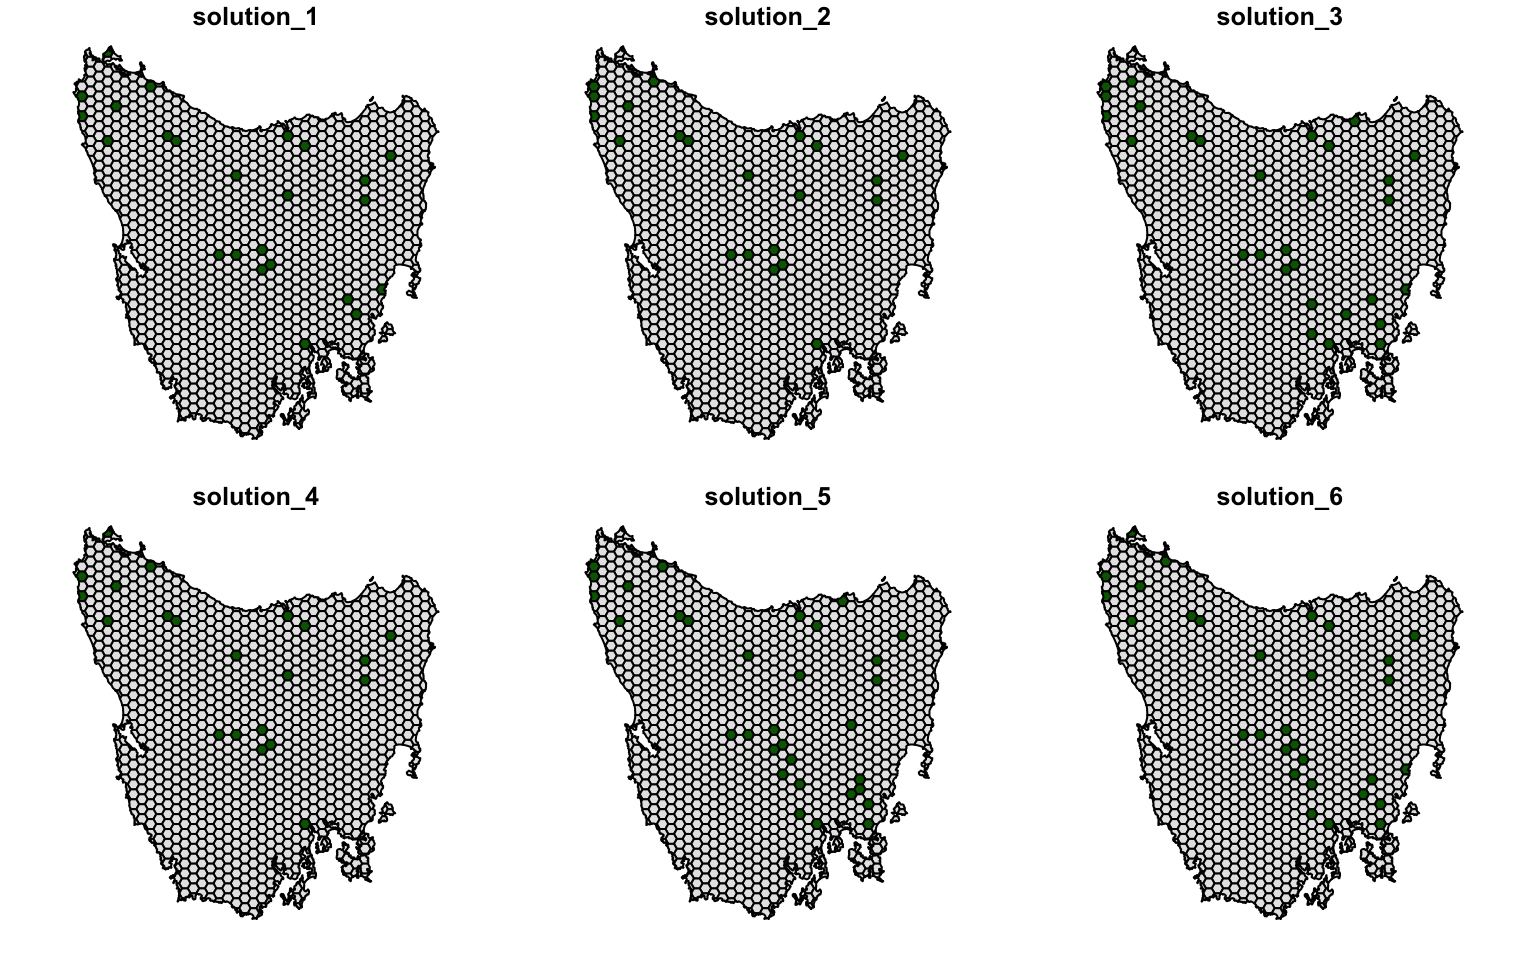
\includegraphics[width=0.65\linewidth]{SpatialPlanning_Workshop2021_files/figure-latex/unnamed-chunk-82-1} \end{center}

\clearpage

\begin{Shaded}
\begin{Highlighting}[]
\CommentTok{\# plot all solutions}
\CommentTok{\# s8\_plots \textless{}{-} lapply(paste0("solution\_", seq\_len(6)), function(x) \{}
\CommentTok{\#   spplot(s8, x, main = x, col.regions = c("white", "darkgreen"))}
\CommentTok{\# \})}
\CommentTok{\# do.call(grid.arrange, append(s8\_plots, list(ncol = 3)))}

\NormalTok{s8}\SpecialCharTok{$}\NormalTok{solution\_1 }\OtherTok{\textless{}{-}} \FunctionTok{factor}\NormalTok{(s8}\SpecialCharTok{$}\NormalTok{solution\_1)}
\NormalTok{s8}\SpecialCharTok{$}\NormalTok{solution\_2 }\OtherTok{\textless{}{-}} \FunctionTok{factor}\NormalTok{(s8}\SpecialCharTok{$}\NormalTok{solution\_2)}
\NormalTok{s8}\SpecialCharTok{$}\NormalTok{solution\_3 }\OtherTok{\textless{}{-}} \FunctionTok{factor}\NormalTok{(s8}\SpecialCharTok{$}\NormalTok{solution\_3)}
\NormalTok{s8}\SpecialCharTok{$}\NormalTok{solution\_4 }\OtherTok{\textless{}{-}} \FunctionTok{factor}\NormalTok{(s8}\SpecialCharTok{$}\NormalTok{solution\_4)}
\NormalTok{s8}\SpecialCharTok{$}\NormalTok{solution\_5 }\OtherTok{\textless{}{-}} \FunctionTok{factor}\NormalTok{(s8}\SpecialCharTok{$}\NormalTok{solution\_5)}
\NormalTok{s8}\SpecialCharTok{$}\NormalTok{solution\_6 }\OtherTok{\textless{}{-}} \FunctionTok{factor}\NormalTok{(s8}\SpecialCharTok{$}\NormalTok{solution\_6)}

\FunctionTok{plot}\NormalTok{(}\FunctionTok{st\_as\_sf}\NormalTok{(s8[, }\FunctionTok{c}\NormalTok{(}\StringTok{"solution\_1"}\NormalTok{, }\StringTok{"solution\_2"}\NormalTok{, }\StringTok{"solution\_3"}\NormalTok{, }\StringTok{"solution\_4"}\NormalTok{, }\StringTok{"solution\_5"}\NormalTok{, }\StringTok{"solution\_6"}\NormalTok{)]),}
  \AttributeTok{pal =} \FunctionTok{c}\NormalTok{(}\StringTok{"grey90"}\NormalTok{, }\StringTok{"darkgreen"}\NormalTok{))}
\end{Highlighting}
\end{Shaded}

\begin{center}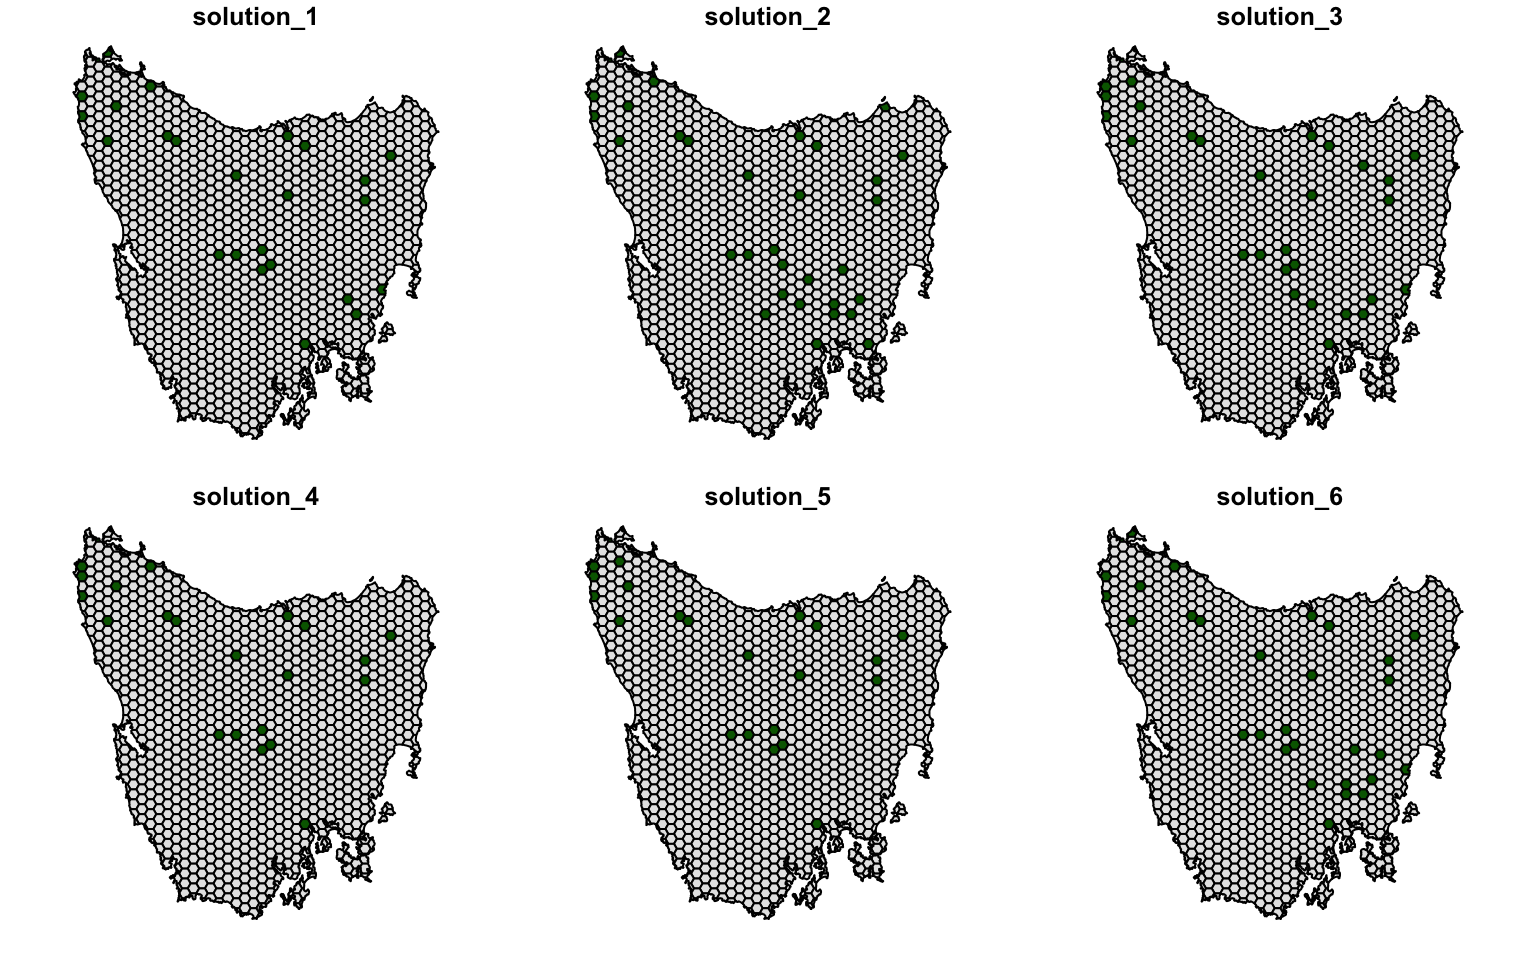
\includegraphics{SpatialPlanning_Workshop2021_files/figure-latex/unnamed-chunk-83-1} \end{center}

\begin{rmdquestion}
\begin{enumerate}
\def\labelenumi{\arabic{enumi}.}
\tightlist
\item
  What is the cost of each of the six solutions in portfolio? Are their costs very different?
\item
  Are the solutions in the portfolio very different?
\item
  What could we do to obtain a portfolio with more different solutions?
\end{enumerate}
\end{rmdquestion}

\hypertarget{acknowledgements}{%
\chapter{Acknowledgements}\label{acknowledgements}}

Many thanks to the \href{https://prioritizr.net/articles/prioritizr.html}{Prioritizr Team} for the development of this software, and for providing the source code for their own workshops so we could more easily develop this one.

Also to Yihui Xie for developing the \href{http://bookdown.org}{bookdown R package} that underpins these notes. We also thank Garrett Grolemund and Hadley Wickham for creating one of the Rstudio screenshots used in this manual that was originally a part of their \emph{R for Data Science} book.

  \bibliography{references.bib}

\end{document}
